
\documentclass{report}
    \title{Deep Learning}
    \author{Timothy Chung}
    \date{8/01/24}

\usepackage[a4paper, total={7in, 10in}]{geometry}
\setlength\parindent{0pt}
%=======================PACKAGES FOR NEWCOMMAND CREATION========================
\usepackage{xparse}
%===============================================================================

%=========================PACKAGES FOR USE IN DOCUMENT==========================
\usepackage[dvipsnames]{xcolor}
\usepackage{graphicx, amssymb, amsfonts, amsmath, listings, multirow, hyperref, mathtools, svg, tikz, enumitem, minted, xfrac, multicol}
\usepackage[most]{tcolorbox}
\usepackage[super]{nth}
\usepackage{tabularx}  % for 'X' column type
\usepackage{multirow}  % for multirow cells
\usepackage{pgfplots}
\pgfplotsset{compat=1.18}
\usetikzlibrary{calc, shapes.geometric, arrows.meta, positioning}

\tikzset{
    neuron/.style={circle, draw, minimum size=1cm},
    input neuron/.style={neuron, fill=gray!20},
    output neuron/.style={neuron, fill=gray!60},
    activation function/.style={
        rectangle,
        draw,
        minimum size=1cm,
        fill=gray!30,
        path picture={
            % Draw the step function inside the activation function node
            \draw[thick] 
            ($(path picture bounding box.south)+(-0.3cm,0.2cm)$) -- 
            ($(path picture bounding box.south)+(0cm,0.2cm)$) -- 
            ($(path picture bounding box.south)+(0cm,0.7cm)$) -- 
            ($(path picture bounding box.south)+(0.3cm,0.7cm)$);
        }
    },
    arrow label/.style={midway, above}
}


% ======= CUSTOM 
\usepackage{subcaption}
\usepackage{wasysym}

%=================================GLOBAL SETUP==================================
\setitemize{itemsep=0em}
%===============================================================================

%===============================INCLUDE CHAPTERS================================
\newcommand{\addchapter}[1]{\include{#1/#1}}
%===============================================================================

%==============================UNFINISHED SECTION===============================
\newcommand{\unfinished}{\begin{huge} \textcolor{red}{\textbf{UNFINISHED!!!}} \end{huge}}
\newcommand{\toimprove}{\begin{huge} \textcolor{olive}{\textbf{NEEDS IMPROVEMENT!!!}} \end{huge}}
%===============================================================================

%==============================PAGE SPLIT LAYOUTS===============================
\NewDocumentCommand{\twosplit}{O{0.48} O{#1} m m}{
	\begin{minipage}[t]{#1\textwidth}
		#3
	\end{minipage}
	\hfill
	\begin{minipage}[t]{#2\textwidth}
		#4
	\end{minipage}
}
%===============================================================================

%============================SPECIAL COLOURED BOXES=============================

% For term definitions
% \begin{definitionbox}{term}
%	... the term's definition ...
% \end{definitionbox}
\newtcolorbox[auto counter,number within=section]{definitionbox}[2][]{%
	colback=blue!5!white,colframe=blue!75!black,arc=0mm,sharp corners=all,fonttitle=\bfseries,%
	title=#2 \hfill Definition \thetcbcounter #1}

% For term definitions
% \begin{sidenotebox}{cool title}
%	... cool unsassessed/not required info ...
% \end{sidenotebox}
\newtcolorbox[auto counter,number within=section]{sidenotebox}[2][]{%
	colback=black!5!white,colframe=black!75!black,arc=0mm,sharp corners=all,fonttitle=\bfseries,%
	title=#2 \hfill \textit{Extra, Not Assessed} \thetcbcounter #1}
% previously the text was "Extra Fun!"

% For example questions:
% \begin{examplebox}{question name}
%   ... the question ...
%	\tcblower
%   ... the worked answer ...
% \end{examplebox}
\newtcolorbox[auto counter,number within=section]{examplebox}[2][]{%
	colback=orange!5!white,breakable,colframe=orange!75!black,arc=0mm,sharp corners=all,fonttitle=\bfseries,%
	title=#2 \hfill Example Question \thetcbcounter #1}

% For exam questions (no answers):
% \begin{exambox}{1c}{2018}
%   ... the question ...
% \end{exambox}
\newtcolorbox[auto counter,number within=section]{exambox}[3][]{%
	colback=purple!5!white,breakable,colframe=purple!75!black,arc=0mm,sharp corners=all,fonttitle=\bfseries,
	title=Q#2 - #3 \hfill Exam Question \thetcbcounter #1}

% For comments:
% \begin{commentbox}
%   ... the question ...
% \end{commentbox}
 
\newtcolorbox[auto counter,number within=section]{commentbox}[2][]{%
    colback=orange!5!white,
    colframe=orange!95!black, % Darker orange frame
    coltitle=white, % White title text
    arc=0mm,
    sharp corners=all,
    fonttitle=\bfseries,
    title=#2 \hfill
}


 

% For positives/pros 
% \begin{prosbox}
%	... the term's definition ...
% \end{prosbox}
\newtcolorbox[]{prosbox}[1][]{%
	colback=green!5!white,breakable,colframe=green!75!black,leftrule=3mm,arc=0mm,sharp corners=all, #1}

% For negatives/cons 
% \begin{prosbox}
%	... the term's definition ...
% \end{prosbox}
\newtcolorbox[]{consbox}[1][]{%
	colback=red!5!white,breakable,colframe=red!75!black,leftrule=3mm,arc=0mm,sharp corners=all, #1}

% For negatives/cons 
% \begin{tabbox}{consbox}
%	... the term's definition ...
% \end{tabbox}
\newenvironment{tabbox}[2][.8\textwidth]{
	\def\boxtype{#2}
	\begin{\boxtype}
		\begin{center}
			\begin{tabular}{r p{#1}}
				}{
			\end{tabular}
		\end{center}
	\end{\boxtype}
}

% \begin{panoptobox}
%   ... the question ...
% \end{panoptobox}
\newtcolorbox{panoptobox}{enhanced,arc=0mm,breakable,sharp corners=all,colback=gray!5,colframe=gray,leftrule=12mm,detach title,%
	underlay unbroken and first={\node[below,text=black,anchor=east] at (interior.base west) {\includegraphics[width=11mm]{../common/images/panopto_logo.png}};}}

\newcommand{\lectlink}[2]{
	\begin{panoptobox}
		\textbf{\href{#1}{#2}}
	\end{panoptobox}
}


% For theorems:
% \begin{theorembox}
%   ... the question ...
% \end{theorembox}
 
\newtcolorbox[auto counter,number within=section]{theorembox}[2][]{%
    colback=red!5!white,
    colframe=red!95!black, % Darker orange frame
    coltitle=white, % White title text
    arc=0mm,
    sharp corners=all,
    fonttitle=\bfseries,
    title=#2 \hfill Theorem \thetcbcounter #1
}


%===============================================================================
\newcommand{\infer}[2]{\cfrac{#1}{#2}}
\newcommand{\infers}[3]{\cfrac{#1}{#2}(#3)}

\newcommand{\ninfer}[3]{(\text{#1}):\cfrac{#2}{#3}}
\newcommand{\ninfers}[4]{(\text{#1}):\cfrac{#2}{#3}(#4)}
\newcommand{\ainfer}[3]{\cfrac{#2}{#3}(\text{#1})}

\newcommand{\mllet}[2]{\text{let } #1 \text{ in } #2}
\newcommand{\mlfix}[2]{\text{fix } #1 . #2}

\newcommand{\hc}{\mathcal{H}}


\begin{document}
\include{titlepage/titlepage}

\begin{titlepage}
    \centering
    \vspace*{1cm}
    \Huge
    \textbf{ELEC60015 Deep Learning} \\
    \vspace{1cm}
    \Large
    Timothy Chung \\
    \vspace{1cm}
    Spring 2024 \\
    \vfill
\end{titlepage}

\setcounter{tocdepth}{1}
\tableofcontents
\newpage
\sn{On The Rigour of A Random Variable}{
For the beginning of this module, a random variable $X$ is considered to be a function from a sample space $\Omega$ to the unit interval $[0, 1]$. However, in Lectures 6 and 7, we use the full definition of a random variable, which is a measurable function from a sample probability space $(\Omega)$ to a measurable space $(E, \varepsilon)$, involving the concept of $\sigma$-algebras and measure spaces. \bigskip

When the sample space is a continuous space, the function $p$ is a \textbf{probability density function} (PDF). When the sample space is a discrete space, the function $p$ is a \textbf{probability mass function} (PMF).
} 


\marginnote[-60pt]{We will introduce measure theory later.}





\section{Brief Probability Theory Review}

$x$ is a sample from a random variable $X$. 

\noindent $P(X=x)$ refers to probability that the random variable $X$ takes on the value $x$.

\subsection{Probability Density Function (PDF)}
\begin{marginfigure}[100pt]
    \centering
    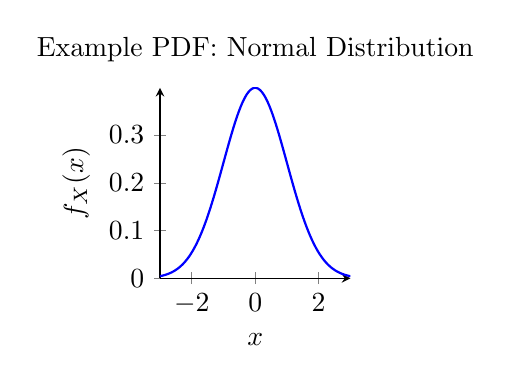
\begin{tikzpicture}
        \begin{axis}[
            width=4cm,
            height=4cm,
            xlabel={$x$},
            ylabel={$f_X(x)$},
            domain=-3:3,
            samples=100,
            axis lines=left,
            ymin=0,
            legend pos=north east,
            title={Example PDF: Normal Distribution}
        ]
        \addplot[blue, thick] {exp(-x^2 / 2) / sqrt(2 * pi)};
        \end{axis}
    \end{tikzpicture}
    \caption{Probability Density Function of a standard normal distribution}
\end{marginfigure}

The Probability Density Function (PDF) of a continuous random variable \(X\) is a function \(f_X(x)\) that describes the relative likelihood for this random variable to take on a given value. The PDF has the following properties:
\begin{itemize}
    \item \(f_X(x) \geq 0\) for all \(x\).
    \item \(\int_{-\infty}^{\infty} f_X(x) \, dx = 1\).
\end{itemize}

Mathematically, the PDF is defined such that the probability that \(X\) lies within a particular interval \([a, b]\) is given by:
\[
P(a \leq X \leq b) = \int_{a}^{b} f_X(x) \, dx.
\]


\subsection{Cumulative Distribution Function (CDF)}
\begin{marginfigure}[50pt]
    \centering
    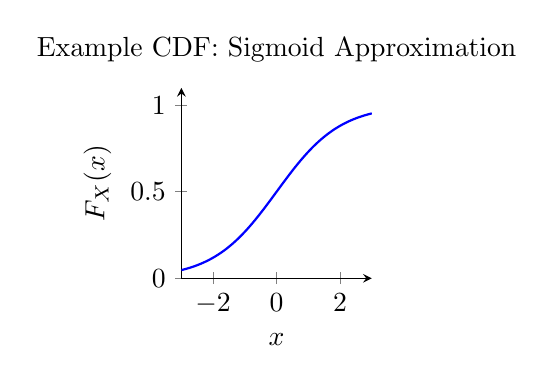
\begin{tikzpicture}
        \begin{axis}[
          width=4cm,
          height=4cm,
            xlabel={$x$},
            ylabel={$F_X(x)$},
            domain=-3:3,
            samples=100,
            axis lines=left,
            ymin=0, ymax=1.1,
            legend pos=south east,
            title={Example CDF: Sigmoid Approximation}
        ]
        \addplot[blue, thick] {1 / (1 + exp(-x))};
        \end{axis}
    \end{tikzpicture}
    \caption{Cumulative Distribution Function}
\end{marginfigure}

The Cumulative Distribution Function (CDF) of a continuous random variable \(X\) is a function \(F_X(x)\) that describes the probability that \(X\) will take a value less than or equal to \(x\). It is defined as:
\[
F_X(x) = P(X \leq x) = \int_{-\infty}^{x} f_X(t) \, dt.
\]

The CDF has the following properties:
\begin{itemize}
    \item \(0 \leq F_X(x) \leq 1\) for all \(x\).
    \item \(F_X(x)\) is a non-decreasing function.
    \item \(\lim_{x \to -\infty} F_X(x) = 0\).
    \item \(\lim_{x \to \infty} F_X(x) = 1\).
\end{itemize}


\subsection{Dealing with Data (Single-Feature)}

In Machine Learning (ML), we often deal with large datasets from which we aim to extract meaningful insights. It is useful to model these data points as random variables:
\[
\{x_1, x_2, \ldots, x_N\}
\]


\noindent We typically model these samples as random variables:

\[
\{x_1 \sim X_1, x_2 \sim X_2, \ldots, x_N \sim X_N\}
\]

\subsection{Vectors of Random Variables}

When dealing with joint random variables, we often represent them as vectors:

\[
\mathbf{X} = (X_1, X_2, X_3) \quad \text{with joint distribution} \quad p_{X_1, X_2, X_3}(x_1, x_2, x_3)
\]

\noindent For a vector of random variables \(\mathbf{X}\) in \( \mathbb{R}^3 \), the joint probability density function is denoted as:

\[
p_{\mathbf{X}}(\mathbf{x}) \quad \text{where} \quad \mathbf{X} \in \mathbb{R}^3
\]
\noindent 
If these are input observations, they are often referred to as "feature vectors."

\subsection{Distinct Random Variables}

We model samples as distinct random variables \sidenote[][-20pt]{\textbf{Why should we model these as distinct random variables? Aren't they all the same thing?} \smallskip

\noindent Despite being identically distributed, distinct random variables allow for capturing dependencies and interactions between different samples.
}:\bigskip

\[
\{x_1 \sim X_1, x_2 \sim X_2, \ldots, x_N \sim X_N\}
\]


\section{Independent and Identically Distributed (i.i.d.) Random Variables}

\marginnote[-50pt]{    \textbf{Why do we model samples as distinct random variables?}

\begin{enumerate}
    \item By treating each sample as a distinct variable, we assume samples are i.i.d, allowing every sample to contribute independently to the likelihood of oberving the data given the model prarameters – so every sample provides unique information to estimate the parameters of the underlying distribution. If we treated all samples as a single random variable, we would lose the granularity of information, leading to a poorer estimate.
    \item Treating samples as distinct allows us to study and model the relationships and dependencies between them.
    \item The assumption of i.i.d follows many results in probability and statistics, such as the Central Limit Theorem, which states that the sum of a large number of i.i.d. random variables is approximately normally distributed. It is also an assumed requirement for a model to generalise. The assumption simplifies the analysis and derivation process, allowing us to use techniques like maximum likelihood estimation (MLE) and empirical risk minimization (ERM).
\end{enumerate}
    }
\subsection{Independence of Random Variables}

Independence refers to the idea that the values or outcomes of one observation in a dataset do not depend on or influence the values of any other observation.\\

For the set of random variables $X_1, X_2, \ldots X_n$, for the collection \[\{x_1 \sim X_1, x_2 \sim X_2, \ldots, x_N \sim X_N\}\]

\noindent we often assume independence, for any subset of observations \(\{X_{i1}, X_{i2}, \ldots, X_{ik}\}\) where \(i_1, i_2, \ldots, i_k \in \{1, 2, \ldots, N\}\), the joint distribution factorises:

\begin{equation}
P(X_{i_1} = x_{i_1}, \ldots, X_{i_k} = x_{i_k}) = P(X_{i_1} = x_{i_1}) \cdot \ldots \cdot P(X_{i_k} = x_{i_k})
\end{equation}

\hl{The joint distribution of the subset is the product of the marginal distributions of the individual random variables.} \bigskip

\textbf{Independence:} The occurrence of any event does not affect the occurrence of others. This is a crucial assumption in many ML models that we will see the usefulness of as early as the next lecture.

\subsection{Identically Distributed Random Variables}

The "identically distributed" part of i.i.d. refers to the idea that all random variables in the sample follow the same probability distribution. That is, they share the same probability density function (pdf) or probability mass function (pmf), depending on whether the data is continuous or discrete. If the set of random variables \(\{X_1, X_2, \ldots, X_n\}\) are identically distributed, then:





\begin{equation}
    f_{X_1}(x) = f_{X_2}(x) = \ldots = f_{X_n}(x) = f_{X}(x)
\end{equation}

\begin{equation}
F_{X_1}(x) = F_{X_2}(x) = \ldots = F_{X_n}(x) = F_{X}(x)
\end{equation}

\noindent This implies that the cumulative distribution function (CDF) is the same for all these random variables.


\section{Statistical Modelling as Curve Fitting}

Machine learning and statistics have significant overlap, and so most concepts studied in this module can be cast as statistical modelling. Consider our random variables:

\begin{equation}
\{x_1 \sim X_1, x_2 \sim X_2, \ldots, x_N \sim X_N\}
\end{equation}

\noindent These random variables can be modelled to fit certain curves that represent the underlying data distribution. 

\subsection{Assumption about the Model}

To proceed with statistical modelling, we make an assumption about the form of the model:

\begin{equation}
P_X(x) \approx \mathcal{N}(x; \theta) \quad \theta := (\mu, \sigma)
\end{equation}

Here, \(P_X(x)\) is approximated by a normal distribution \(\mathcal{N}(x; \theta)\), where \(\theta\) represents the parameters of the distribution, namely the mean \(\mu\) and the standard deviation \(\sigma\). This assumption simplifies the process of modelling the data.

\subsection{Fitting the Model}

The next step is to fit the model to the data. This involves finding the parameter values \(\theta\) that maximize the probability of observing the given data. Mathematically, this is expressed as:

\begin{equation}
\arg \max_{\theta} P(x_1, \ldots, x_N \mid \theta)
\end{equation}

In other words, we adjust the parameters \(\mu\) and \(\sigma\) so that the assumed model best fits the observed data. This process is known as maximum likelihood estimation (MLE).\\











\section{Discrete Random Variables}


\subsection{Bernoulli and Multinoulli Distributions}
\textbf{Bernoulli Distribution:} Outcome with two values (e.g., heads or tails).
\begin{itemize}
    \item Parameter: \(\theta\).
    \item Probabilities: \(P(X = 0) = 1 - \theta\), \(P(X = 1) = \theta\).
\end{itemize}

\textbf{Multinoulli Distribution:} Describes a scenario with multiple possible outcomes, extending the Bernoulli distribution to more than two outcomes.
\begin{itemize}
    \item Parameter: \(\bm{\theta} \in \mathbb{R}^s\) where each \(\theta_i\) represents the probability of the \(i\)-th outcome, and \(\sum_{i=0}^{s-1} \theta_i = 1\).
    \item Probabilities: \(P(X = i) = \theta_i\) for \(i = 0, 1, \ldots, s-1\).
\end{itemize}

\subsection{Binomial and Multinomial Distributions}
\textbf{Binomial Distribution:} \(X \sim \text{Bin}(n, \theta)\).
\begin{itemize}
    \item Probability Mass Function (p.m.f):
    \[
    \text{Bin}(k \mid n, \theta) := \binom{n}{k} \theta^k (1 - \theta)^{n-k}
    \]
    \item Binomial Coefficient:
    \[
    \binom{n}{k} = \frac{n!}{(n - k)!k!}
    \]
    \item Mean: \(n\theta\).
    \item Variance: \(n\theta(1 - \theta)\).
\end{itemize}

\textbf{Multinomial Distribution:} Generalises the binomial distribution for more than two outcomes. It models the probabilities of counts among multiple categories in \(n\) independent trials.
\begin{itemize}
    \item Parameters: \(n\) (number of trials) and \(\boldsymbol{\theta} = (\theta_1, \theta_2, \ldots, \theta_K)\) where \(\theta_i\) is the probability of the \(i\)-th category and \(\sum_{i=1}^{K} \theta_i = 1\).
    \item Probability Mass Function (p.m.f):
    \[
    \text{Mu}(\mathbf{x} \mid n, \boldsymbol{\theta}) := \binom{n}{x_1, x_2, \ldots, x_K} \prod_{j=1}^{K} \theta_j^{x_j}
    \]
    where \(\mathbf{x} = (x_1, x_2, \ldots, x_K)\) represents the count of occurrences for each category.
    \item Multinomial Coefficient:
    \[
    \binom{n}{x_1, x_2, \ldots, x_K} = \frac{n!}{x_1! x_2! \cdots x_K!}
    \]
    \item Mean for each category \(i\): \(\mathbb{E}[X_i] = n\theta_i\).
    \item Variance for each category \(i\): \(\text{Var}(X_i) = n\theta_i(1 - \theta_i)\).
    \item Covariance between categories \(i\) and \(j\): \(\text{Cov}(X_i, X_j) = -n\theta_i\theta_j\).
\end{itemize}


\subsection{Empirical Distribution}
\defb{Empirical Distribution}{
Based on observation or experience rather than theory or pure logic.
}


\begin{intuitbox}{Empirical Distribution}
    

    Practically, we do not have access to an infinite amount of data, but we have instead a small fraction of it, a sample, to infer any insights from it. In the case of discrete random variables, we use probability mass functions, which is straightforward, but we are interested in probability density functions for continuous random variables, because to model the true distribution, we would need an infinite number of samples. \bigskip

    Thus, our goal is to approximate the true PDF from a given data set using finite samples. The transformation from discrete to continuous is done with the Dirac delta function.\\ \bigskip

    A Dirac delta function is interestingly helpful because:
    \[
    \int_{-\infty}^{\infty} \delta(x) \, dx = 1
    \]

    We can then have multiple Dirac delta functions to represent the empirical distribution of a data set, but scaled down by a factor equivalent to the total number of data points to ensure the area under the curve is 1.\\

    \begin{center}
        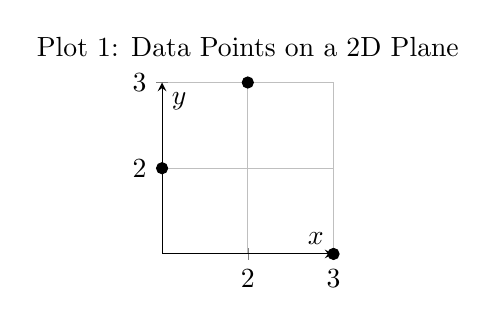
\begin{tikzpicture}
            \begin{axis}[
                title={Plot 1: Data Points on a 2D Plane},
                xlabel={$x$},
                ylabel={$y$},
                axis lines=middle,
                grid=major,
                width=0.31\textwidth,
                height=0.31\textwidth,
                xtick={1, 2, 3},
                ytick={0, 1, 2, 3}
            ]
                \addplot[only marks, mark=*, mark size=2pt] coordinates {(1,2) (2,3) (3,1)};
            \end{axis}
        \end{tikzpicture}
        \hspace{1cm}
        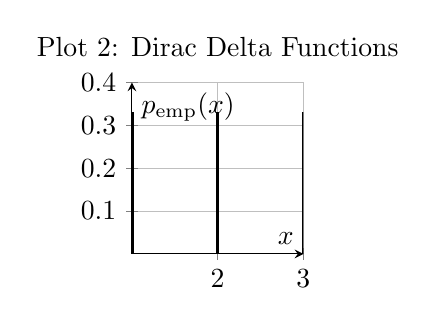
\begin{tikzpicture}
            \begin{axis}[
                title={Plot 2: Dirac Delta Functions},
                xlabel={$x$},
                ylabel={$p_{\text{emp}}(x)$},
                axis lines=middle,
                grid=major,
                width=0.31\textwidth,
                height=0.31\textwidth,
                ymin=0, ymax=0.4,
                xtick={1,2,3},
                ytick={0,0.1,0.2,0.3,0.4}
            ]
                \addplot[very thick] coordinates {(1,0) (1,0.33)};
                \addplot[very thick] coordinates {(2,0) (2,0.33)};
                \addplot[very thick] coordinates {(3,0) (3,0.33)};
            \end{axis}
        \end{tikzpicture}
        \hspace{1cm}
        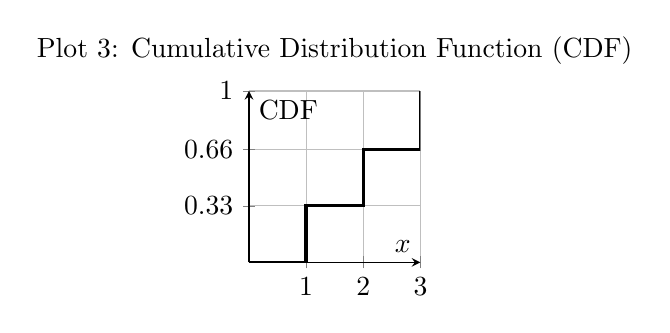
\begin{tikzpicture}
            \begin{axis}[
                title={Plot 3: Cumulative Distribution Function (CDF)},
                xlabel={$x$},
                ylabel={CDF},
                axis lines=middle,
                grid=major,
                width=0.31\textwidth,
                height=0.31\textwidth,
                ymin=0, ymax=1,
                xtick={1, 2, 3},
                ytick={0, 0.33, 0.66, 1}
            ]
                \addplot[very thick] coordinates {(0,0) (1,0) (1,0.33) (2,0.33) (2,0.66) (3,0.66) (3,1)};
            \end{axis}
        \end{tikzpicture}
    \end{center}
    
\end{intuitbox}

\marginnote[-120pt]{    \refsb{Recommended Viewing}{
  \href{https://www.youtube.com/watch?v=7f3YFT7bsmg}{Lecture on Empirical Distribution}\smallskip

  Empirical Statistics: When you compute statistics from a dataset, you're really computing statistics for its empirical distribution.\smallskip

  A dataset is, in essence, a distribution.
}}


\textbf{Empirical Distribution:} Suppose we have a set of data samples 

$$D = \{x^{(1)}, x^{(2)}, \ldots, x^{(N)}\} $$

derived from a random variable \(X\). We can approximate the distribution of \(X\) using a set of delta functions on these samples:
% Represents the distribution of a given data set \(D = \{x^{(1)}, \ldots, x^{(N)}\}\).
\begin{itemize}
    \item For a given data set \(D\), the empirical distribution \(p_{\text{emp}}(x)\) is defined as:
    \[
    p_{\text{emp}}(x) := \frac{1}{N} \sum_{i=1}^N \delta_{x_i}(x)
    \]
    where \(\delta_{x_i}(x)\) is the Dirac measure centred at \(x_i\).
    \item \textbf{Dirac Measure:} \(\delta_{x_i}(x)\) is a function that is 1 if \(x = x_i\) and 0 otherwise. Formally, it is defined as:
    \[
    \delta_{x_i}(x) = \begin{cases} 
    1, & \text{if } x = x_i \\
    0, & \text{if } x \neq x_i 
    \end{cases}
    \]
    \item Explanation: The empirical distribution assigns equal probability \( \frac{1}{N} \) to each observed data point \(x_i\). It is a discrete distribution that places mass only on the observed data points.
    \item In general, one can associate weights with each element of the empirical distribution, i.e., \(p_{\text{emp}}(x) = \frac{1}{N} \sum_{i=1}^N w_i \delta_{x_i}(x)\) as long as each \( 0 \leq w_i \leq 1 \) and \( \sum_{i=1}^N w_i = 1 \).
\end{itemize}

\section{Continuous Random Variables}

\subsection{Gaussian (Normal) Distribution}
\textbf{Probability Density Function (p.d.f):}
\begin{itemize}
    \item Formula: \[
    N(x \mid \mu, \sigma^2) = \frac{1}{\sqrt{2\pi\sigma^2}} \exp\left(-\frac{(x - \mu)^2}{2\sigma^2}\right)
    \]
    \item Mean: \(\mu = \mathbb{E}[X]\).
    \item Variance: \(\sigma^2 = \text{Var}[X]\).
    \item Standard Normal Distribution: \(X \sim N(0, 1)\).
    \item Precision: \(\lambda = \frac{1}{\sigma^2}\).
\end{itemize}
\textbf{Cumulative Distribution Function (CDF):}
\begin{itemize}
    \item Formula: \[
    \Phi(x; \mu, \sigma^2) = \int_{-\infty}^x N(z; \mu, \sigma^2) \, dz
    \]
    \item In terms of the error function (erf):
        \[
        \Phi(x; \mu, \sigma^2) = \frac{1}{2} \left[1 + \text{erf}\left(\frac{z}{\sqrt{2}}\right)\right]
        \]
        where \(z = \frac{x - \mu}{\sigma}\) and
        \[
        \text{erf}(x) = \frac{1}{\sqrt{\pi}} \int_0^x \exp(-t^2) \, dt
        \]
\end{itemize}


\section{Viewing Data}

\begin{itemize}
    \item Data (coordinates) Perspective (Design Matrix) 
    \item Set Perspective
    \begin{itemize}
        \item Combination invariant
        \item Allows for natural language....??
    \end{itemize}
    \item Empirical Distribution Perspective
    \begin{itemize}
        \item i.i.d
    \end{itemize}
\end{itemize}


\section{Example Scene: Self-Driving Car}
\sn{Notation and Gotchas}{
    The lecture use $x_i$ to denote the $i$-th feature, and $x^{(i)}$ to denote the $i$-th data point. The slides however seem to denote $x_i$ as the $i$-th data point. The notes follow the former convention.\\

    Also, it is generally assumed that in a classification problem, the classes are distinct and mutually exclusive, so an image is either a dog or a cat (multi-class classfication) but not a combination of both (multi-label classification). The course focuses on the former convention.

}
Take a case of the self-driving car. There are several facets:
\begin{enumerate}
    \item \textbf{Object Recognition: }identifying objects in the scene (classification)
          \begin{itemize}[noitemsep]
              \item An image is a 2D array of pixel values. For a colour image, each pixel has 3 values (RGB).
              \item \textbf{Input:}
                    \begin{equation}
                        x \in \mathbb{R}^{H \times W \times C}
                    \end{equation}
                    where $H$ is height, $W$ is width, and $C$ is the number of channels (e.g. 3 for RGB)
              \item \textbf{Output:} We would like to detect if something is a background, another vehicle, the ground level, or a pedestrian. Let's say there are $m$ outcomes, making this a \textbf{classification problem}. Naively, let
                    $y \in \mathbb{R}^m$. However, these numbers are just arbitrary i.e. raw scores. It would make more sense to refine the output to a probability distribution over the $m$ classes: \\
                    \begin{equation}
                        y \in \Delta^m \quad \text{where }\sum_{i=1}^{m} y_i = 1
                    \end{equation}
                    Where the $\Delta^m$ is the $m$-simplex, where the sum of all elements is 1. This provides a measure of ``confidence'' in the prediction. Example: To choose between four classes: [Vehicle, Pedestrian, Road, Background], the output could be $[0.1, 0.7, 0.1, 0.1]$. This means the model is 70\% confident that the object is a pedestrian.
              \item \textbf{Our objective is to learn a function:}
                    \begin{equation}
                        f^\theta : x^{(i)} \mapsto y^{(i)} \quad \text{where } \theta \text{ are model parameters}, x^{(i)} \in \mathbb{R}^{H \times W \times C}, y^{(i)} \in \Delta^m
                    \end{equation}
                    \begin{marginfigure}
                        \centering
                        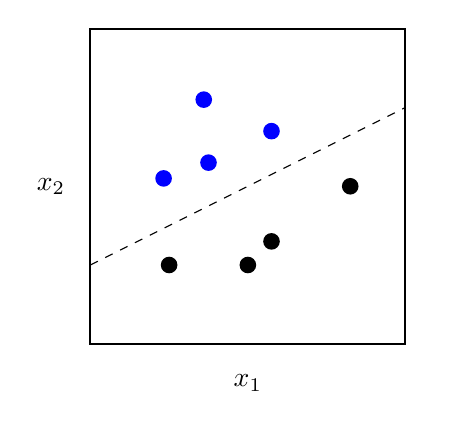
\begin{tikzpicture}
                            % Draw the outer square
                            \draw[thick, black] (0,0) rectangle (4,4);
                            % Draw the blue points
                            \fill[blue] (1.44,3.1) circle (3pt);
                            \fill[blue] (1.5,2.3) circle (3pt);
                            \fill[blue] (0.93,2.1) circle (3pt);
                            \fill[blue] (2.3,2.7) circle (3pt);
                            % Draw the black points
                            \fill[black] (3.3,2) circle (3pt);
                            \fill[black] (2.3,1.3) circle (3pt);
                            \fill[black] (2,1) circle (3pt);
                            \fill[black] (1,1) circle (3pt);
                            % Labels for the axes
                            \node at (2,-0.5) {$x_1$};
                            \node at (-0.5,2) {$x_2$};
                            % Dashed separator
                            \draw[dashed] (0,1)--(4,3) node[right] {};
                        \end{tikzpicture}
                        \caption{Simplified example for $f^\theta$}
                        \label{fig:1_classification}
                    \end{marginfigure}
                    A simplified example for $f^\theta$ is shown in Figure \ref{fig:1_classification}. Ideally, we want a separator that separates the input space into $m$ distinct regions according to observed data.

              \item \textbf{Data Formalisation (1): }We can view our dataset as a set of $N$ pairs where $x^{(i)}$ is an image and $y^{(i)}$ is the corresponding label. More neatly put,
                    \begin{equation}
                        \mathcal{D} = \{(x^{(i)}, y^{(i)})\}_{i=1}^{N}, \quad x^{(i)} \in \mathbb{R}^{H \times W \times C}, y^{(i)} \in \Delta^m
                    \end{equation}
              \item \textbf{Data Formalisation (2): } We could also view the dataset as an empirical distribution over the data space like in Figure \ref{fig:1_distribution}:
                    \begin{equation}
                        \mathcal{D} = \{x^{(i)}, y^{(i)}\}_{i=1}^{N} \sim p_{\text{data}}(x, y)
                    \end{equation}
                    \begin{marginfigure}
                        \centering
                        \begin{tikzpicture}
                            \begin{axis}[
                                view={0}{90},
                                axis on top,
                                enlargelimits=false,
                                colormap/viridis,
                                xlabel={$x_1$},
                                ylabel={$x_2$},
                                % colorbar,
                                samples=50, % Adjusting the sample size
                                domain=-5:5,
                                width=2in,
                                height=2in
                            ]
                            
                            % First contour group
                            \addplot3[
                                contour gnuplot={
                                    levels={0.25, 0.4, 0.55, 0.65, 0.79, 1, 1.25, 1.5}
                                }
                            ]
                            {exp(-((x)^2 + (1.4*y)^2))};
                    
                            % Second contour group
                            \addplot3[
                                contour gnuplot={
                                    levels={0.25, 0.4, 0.55, 0.65, 0.79, 1, 1.25, 1.5}
                                }
                            ]
                            {exp(-((2*x+2)^2 + (y+2)^2))};
                            
                            \end{axis}
                        \end{tikzpicture}
                        \caption{Viewing the dataset as an empirical distribution}
                        \label{fig:1_distribution}
                    \end{marginfigure}
                    



          \end{itemize}
          \item \textbf{Route Planning:} 
          We aim to predict the optimal path, where the prediction function \( f^\theta \) takes spatial data and environmental conditions as input and outputs a route (either as a series of decisions or waypoints).
          \begin{itemize}[noitemsep]
              \item \textbf{Input:}
              \begin{equation}
                  x \in \mathbb{R}^{n}
              \end{equation}
              where \( x \) could represent a vector of features including road conditions, traffic density, and start/end coordinates.
              
              \item \textbf{Output:} 
              A route \( y \), represented either as a classification over a set of discrete routes, or as continuous waypoints:
              \begin{equation}
                  f^\theta : x \mapsto y
              \end{equation}
              Here, \( y \in \mathbb{R}^m \) for \( m \) possible waypoints (or classes, if we use a discrete route classification).
          \end{itemize}
          The objective is to minimise the difference between predicted and actual routes, defined as a suitable loss function \( \mathcal{L}(f^\theta(x), y) \).

    \item \textbf{Speed Control:} 
    \sn{Ordinal Regression here?}{To update}
          In this problem, we predict the optimal driving speed, and \( f^\theta \) models the relationship between environmental and driving conditions and speed.
          \begin{itemize}[noitemsep]
              \item \textbf{Input:} 
              \begin{equation}
                  x \in \mathbb{R}^p
              \end{equation}
              where \( x \) represents features such as current speed, distance to obstacles, road surface, and weather conditions.
              
              \item \textbf{Output:} 
              A continuous speed value \( y \in \mathbb{R} \):
              \begin{equation}
                  f^\theta : x \mapsto y
              \end{equation}
              where \( y \) is the predicted speed. This is a regression problem, so the goal is to minimise the squared error:
              \begin{equation}
                  \mathcal{L}(\theta) = \frac{1}{N} \sum_{i=1}^{N} (f^\theta(x^{(i)}) - y^{(i)})^2
              \end{equation}
          \end{itemize}

    \item \textbf{Steering Angle Prediction:}
          Steering angle prediction aims to output a continuous angle based on the driving conditions, making it a regression problem.
          \begin{itemize}[noitemsep]
              \item \textbf{Input:}
              \begin{equation}
                  x \in \mathbb{R}^q
              \end{equation}
              where \( x \) could represent lane position, vehicle surroundings, and road curvature.
              
              \item \textbf{Output:} 
              The predicted steering angle \( y \in \mathbb{R} \):
              \begin{equation}
                  f^\theta : x \mapsto y
              \end{equation}
              This is also a regression task, and the loss function could again be the squared error:
              \begin{equation}
                  \mathcal{L}(\theta) = \frac{1}{N} \sum_{i=1}^{N} (f^\theta(x^{(i)}) - y^{(i)})^2
              \end{equation}
          \end{itemize}
\end{enumerate}

\section{Mathematics of Linear Models}

Linear models are fundamental in statistics and supervised machine learning. They can:
\begin{itemize}[noitemsep]
    \item Handle linear relationships.
    \item Be augmented with kernels or basis functions to model non-linear relationships.
    \item Provide analytical tractability for studying concepts like convergence, probabilistic modelling, and overfitting.
\end{itemize}
This section introduces the linear regression model.

\subsection{Linear Regression Model}

Linear regression involves performing regression with a linear model in a supervised setting. Given a dataset \(\mathcal{D}\) consisting of input-output pairs \((\bm{x}^{(i)}, y^{(i)})\) for \(i = 1, \ldots, N\):
\begin{itemize}[noitemsep]
    \item \(\bm{x} \in \mathbb{R}^n\) represents the input features.
    \item \(y \in \mathbb{R}\) represents the output or target variable.
    \item Assume a domain \(\mathbb{R}^n\) and a one-dimensional co-domain.
    \item Model: \(f(\bm{x}) = \bm{x}^\top \bm{\theta}\).
    \item Noise: \(\epsilon \sim \mathcal{N}(0, \sigma^2)\).
\end{itemize}
The full model is:
\[
\hat{y}^{(i)} = \bm{x}^{(i)\top} \bm{\theta} + \epsilon
\]

The objective is to find \(\bm{\theta}\) such that \(\hat{y}^{(i)} \approx y^{(i)}\). In other words, we want to find a set of parameters \(\bm{\theta}\) that best explains the relationship between the input features \(\bm{x}\) and the target variable \(y\). This means minimising the difference between the predicted values \(\hat{y}\) and the actual values \(y\).\bigskip

\textbf{Conventions and Notations:}
\begin{itemize}[noitemsep]
    \item Vectors \(\bm{x} \in \mathbb{R}^n\) are column vectors, written as \(n \times 1\) matrices.
    \item \(\bm{x}^\top\) (x transpose) swaps rows and columns of \(\bm{x}\), resulting in a \(1 \times n\) row vector.
\end{itemize}




\begin{referencebox}{Lecture Reading}
    Chapter 1-2 of Kevin Murphy's \textit{Machine Learning: A Probabilistic Perspective}. Chapter 1.4 was not covered, but may be of interest
\end{referencebox}





\chapter{Convolutional Neural Networks}
\begin{figure}[H]
    \centering
    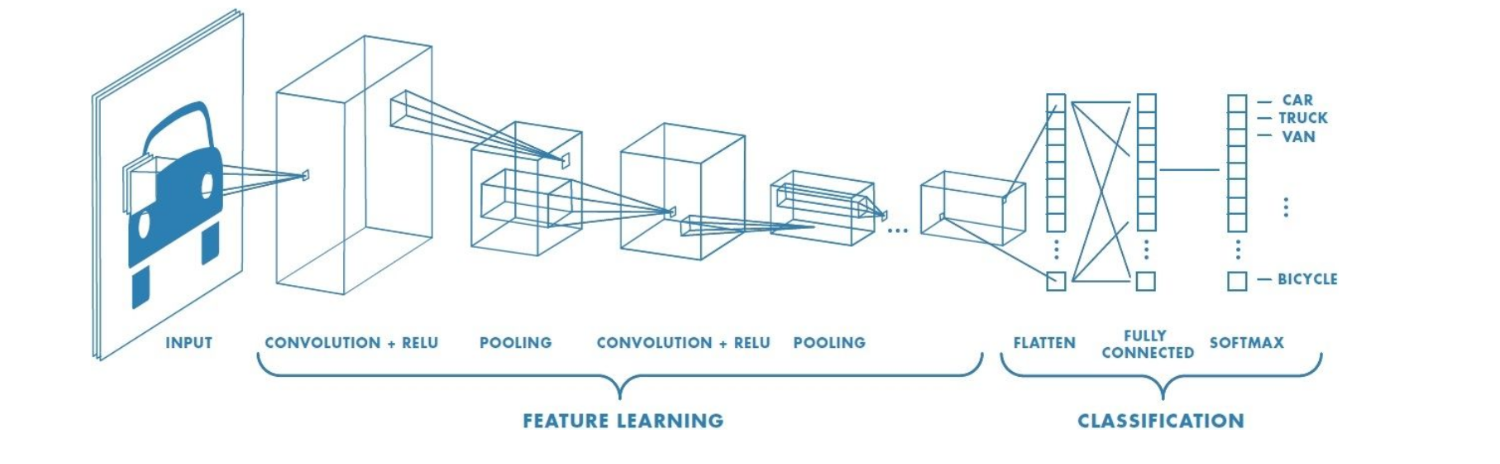
\includegraphics[width=0.75\linewidth]{img/CNN_diagram.png}
\end{figure}


\section{Introduction}

 CNNs are a specialised kind of neural network that are designed to process data that comes in the form of multiple arrays, such as colour images composed of 2D pixel arrays for each colour channel.

\section{CNN Architecture}

The architecture of a CNN is engineered to take advantage of the 2D structure of an input image, performing convolution on its input as form of feature extraction. This involves sliding filter matrices, or kernels, across the input data to produce feature maps that summarise the presence of detected features in the input.

Key components of CNNs include:

\begin{itemize}
    \item \textbf{Convolutional layers:} These layers apply a number of filters to the input. Each filter detects different features by performing a convolution operation.
    \item \textbf{Filters and Feature Maps:} Filters are small, learnable weights that convolve over the input to produce feature maps, representing detected features.
    \item \textbf{Strides:} The stride defines the step size the filters take during the convolution operation across the input.
    \item \textbf{Padding:} Padding can be added to the input volume to allow the filter to cover the border of the input, thereby adjusting the spatial size of the output volume.
    \item \textbf{Pooling layers:} These layers reduce the dimensions of the data by combining the outputs of neuron clusters at one layer into a single neuron in the next layer.
    \item \textbf{Fully Connected (FC) layers:} After several convolutional and pooling layers, the high-level reasoning in the neural network is done via fully connected layers. Neurons in a fully connected layer have full connections to all activations in the previous layer.
    \item \textbf{Loss layers:} At the end of the network, a loss layer defines how the network's predictions are compared to the true data labels for the purpose of learning during training.
\end{itemize}
\section{CNN Overview and Input Data}
\begin{itemize}
    \item \textbf{Neural Network Architecture Optimisation:} CNNs are optimised for k-D data structures like images, including RGB or hyperspectral images.
    \item \textbf{Tensor Representation:} An image is represented as a 4D tensor with dimensions corresponding to the number of samples, height, width, and color channels of the input data.
    \item \textbf{Local Correlation:} Due to the nature of images, neighbouring pixels are often correlated, and this spatial correlation is leveraged by CNNs to reduce the number of parameters and computational complexity.
\end{itemize}



Images are represented as 4D tensors in CNNs: (samples, height, width, channels).\\

\begin{commentbox}{What's a Tensor?}
    
A tensor is a mathematical object that can be thought of as a generalised form of matrices. A tensor can have multiple dimensions, often referred to as ``axes". Each dimension of a tensor can represent different aspects of the data. 

\begin{itemize}
    \item0D Tensor (Scalar): A single number. For example, 5 or -3.2.
    \item1D Tensor (Vector): An array of numbers. For example, [1, 2, 3].
    \item2D Tensor (Matrix): An array of arrays of numbers. For example, [[1, 2, 3], [4, 5, 6]].
    \item3D Tensor: An array of matrices. In image processing, a 3D tensor can represent a color image where there are three matrices corresponding to the Red, Green, and Blue (RGB) color channels. This would look like: 
    \[
    \begin{bmatrix}
        [100,0,230] & [255,255,0] & [12,70,123]\\
        [12,5,1] & [89,4,12] & [123,6,82]\\
        [0,0,0] & [255,255,255] & [204,211, 90]
    \end{bmatrix}
    \]
    \item4D Tensor: Used in CNNs to store a batch of images. Each `slice' of this 4D tensor is a 3D tensor representing one image.
\end{itemize}
\end{commentbox}

These dimensions correspond to the number of samples in a batch, the image height, the image width, and the number of colour channels.\\

Filter convolutions are performed as shown in the diagram below:
\begin{figure}[H]
    \centering
    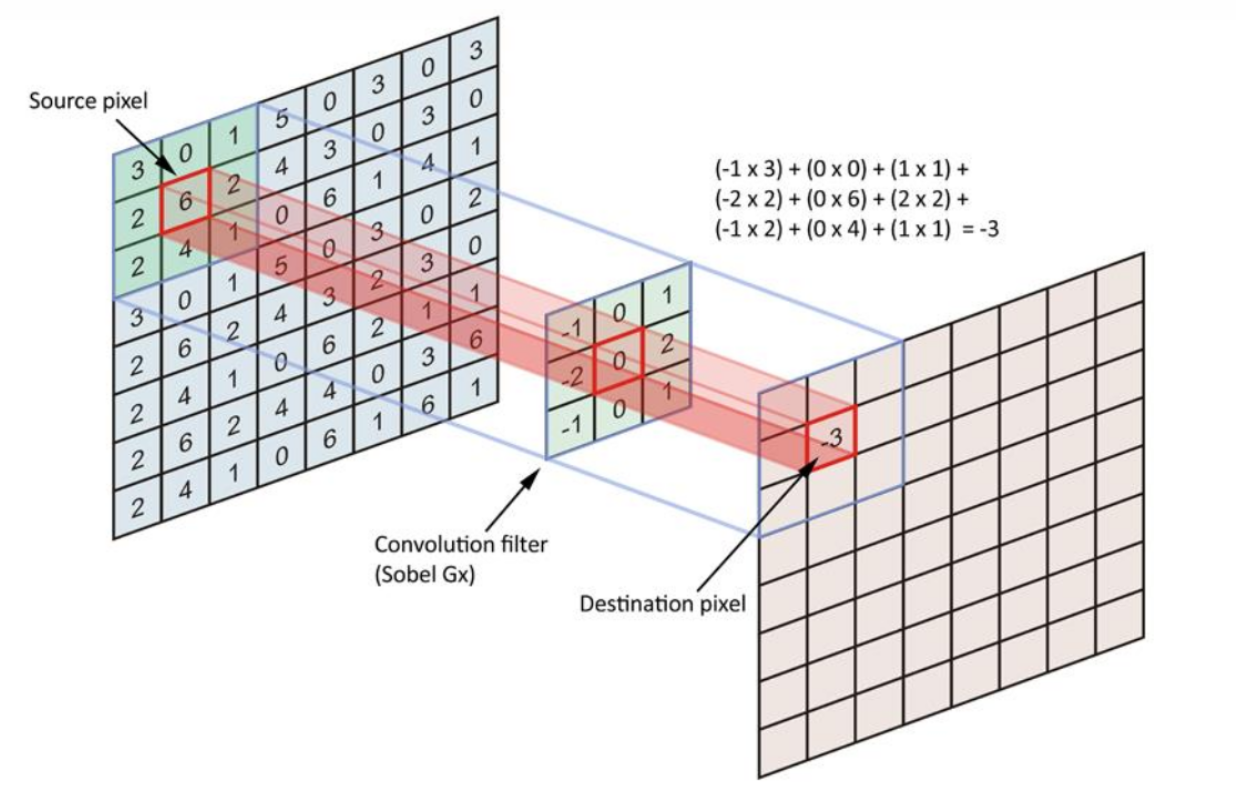
\includegraphics[width=0.75\linewidth]{img/CNN_filter.png}
    
    
\end{figure}

Now assume we have a \(30 \times 30 \times 3\) image. We reserve a 5-level filter for each pixel. Each filter has a  \(7 \times 7\) input. Spatially, we can arrange \(30 {\color{teal}+1}-7 = 24\)  filters across the x-axis so they receive a unique input, and the same for the y-axis. Each filter has \( 7 \times 7 \times 3\) parameters. As we have a depth of 5 levels, we multiply again. \\

\begin{figure}[H]
    \centering
    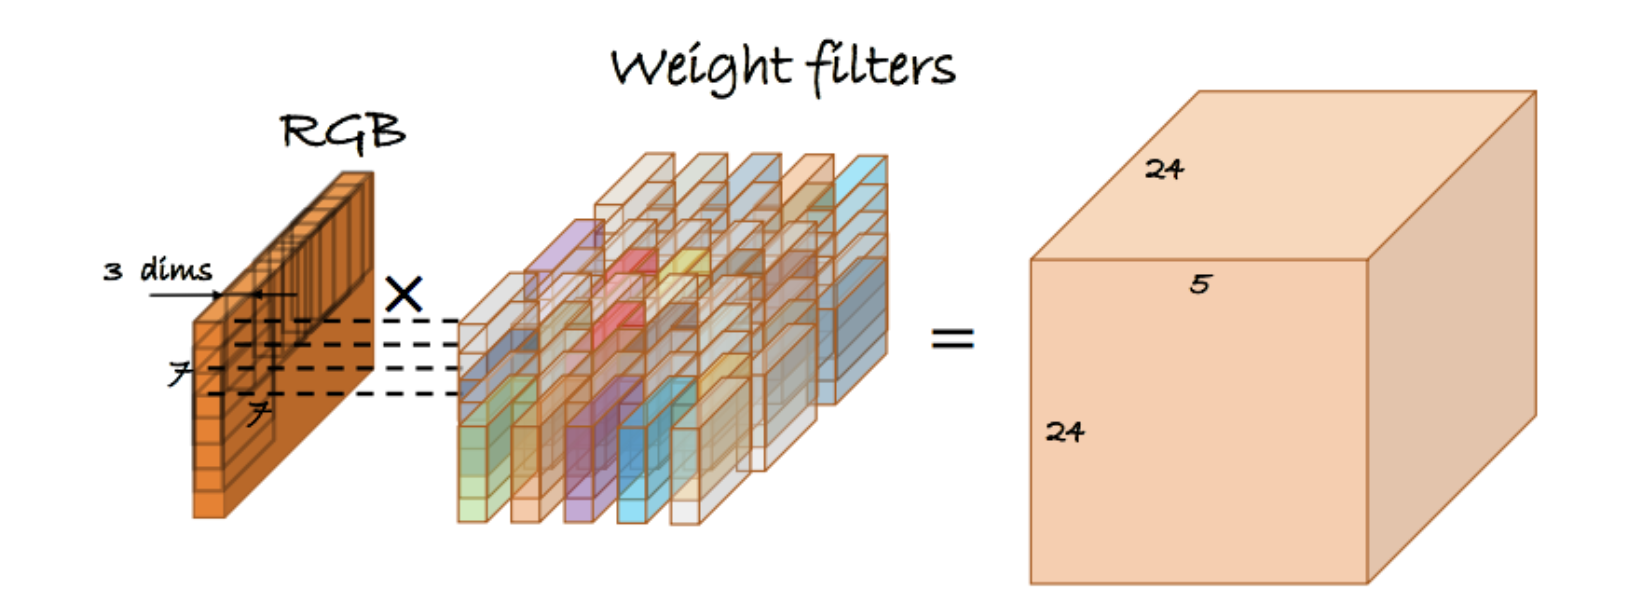
\includegraphics[width=0.75\linewidth]{img/cnn_1.png}
    
    
\end{figure}

The total number of parameters is:
\[
\underbrace{24}_{\text{x-axis}} \times \underbrace{24}_{\text{y-axis}} \times \underbrace{ 7 \times 7 \times 3}_{\text{filter parameters}} \times \underbrace{5}_{\text{filter depth}} = 423\text{k parameters}
\]

(To find out why we {\color{teal}+1}, try visualise this with a simpler example, like \(2 \times 2\) filters on a \(4 \times 4\) image.)

To which, we see the need for an excessive amount of parameters. If we had a \(256 \times 256\) image, we would need \(46 \times 10^6\) parameters.\\

We can do better by repeating filters as a sliding window. Now these filters are transient.

\begin{figure}[H]
    \centering
    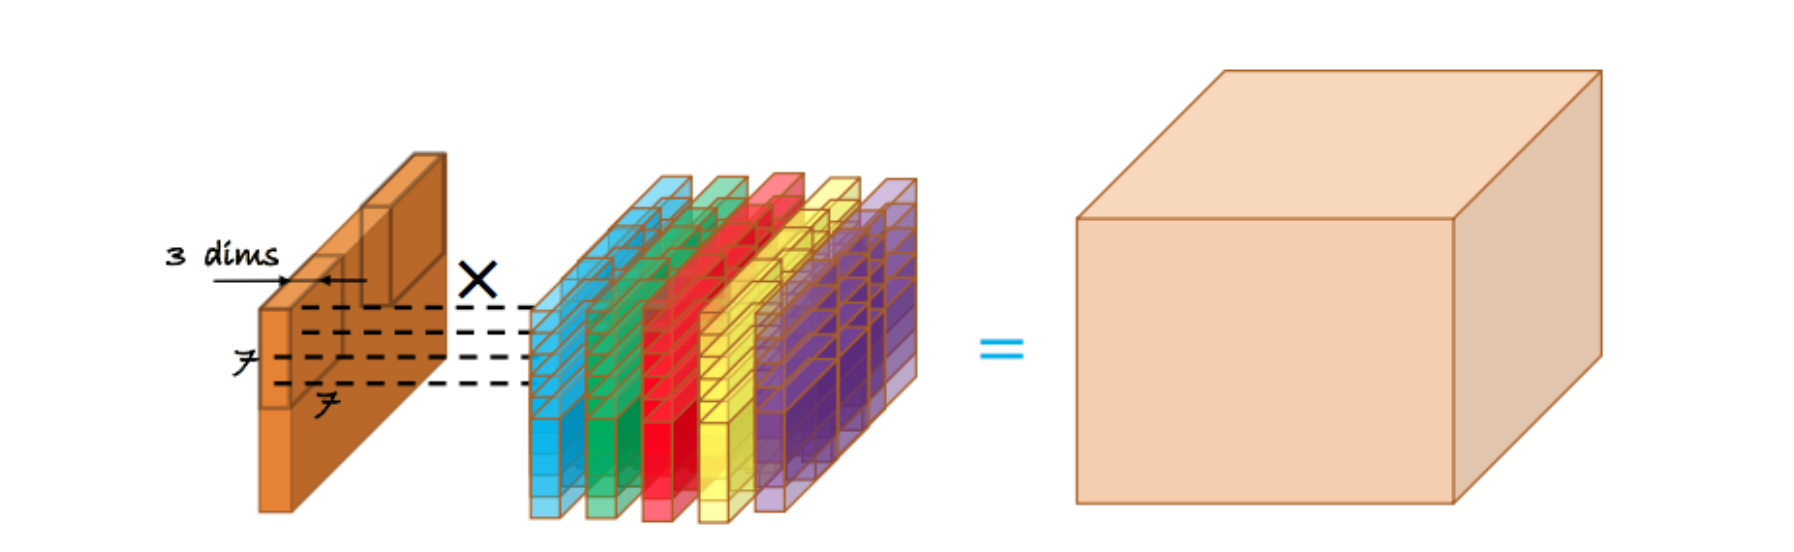
\includegraphics[width=0.75\linewidth]{img/cnn_2.png}
    
    
\end{figure}

The total number of parameters is now:
\[
 \underbrace{ 7 \times 7 \times 3}_{\text{filter parameters}} \times \underbrace{5}_{\text{filter depth}} = 735\text{ parameters}
\]

More generally, the output size, is computed by:

\[
    H_o = H_i - K + 1
\]

Where \(H_o\) is the output height, \(H_i\) is the input height, K is the kernel(filter) size.


\section{Convolution}

Convolution is a mathematical operation that is central to convolutional neural networks. It serves as a tool for feature extraction and is used to process data by applying a filter or kernel.

\subsection{Convolution in Continuous Space}

The convolution operator is defined in the continuous space as an integral transform. It is given by the integral of the product of two functions after one is reversed and shifted:

\[
(f * w)(t) = \int_{-\infty}^{+\infty} f(\tau) w(t - \tau) d\tau
\]

This operation can be understood as a weighted average of the function \( f \) across time or space, using the weighting function \( w \), which is the filter or kernel. The result is a new function that expresses how the shape of one function is modified by the other.

\subsection{Discrete Convolution}

In digital applications where signals are represented discretely, convolution is implemented as a sum:

\[
(f * w)(t) = \sum_{\tau=-\infty}^{+\infty} f(\tau) w(t - \tau)
\]

In practice, since signals and kernels are finite, the bounds of summation are limited to the extent of the defined functions.

\subsection{1D and 2D Discrete Convolution}

For a one-dimensional discrete signal, the convolution is a sum over the product of two discrete functions, one of which is flipped and shifted:

\[
(x * F)(i) = \sum_m x(m) F(i - m)
\]

In two dimensions, which is the common case for image processing, the convolution is a sum over both dimensions:

\[
(x * F)(i, j) = \sum_m \sum_n x(m, n) F(i - m, j - n)
\]

Alternatively, if we consider \( x \) as the input and \( F \) as the kernel or filter, the 2D convolution can also be expressed as:

\[
(x * F)(i, j) = \sum_m \sum_n x(i + m, j + n) F(m, n)
\]

The choice of the convolution expression can depend on the indexing convention, but the core concept remains the same. Different convolutions can create feature maps that highlight important features such as edges, textures, and shapes that are essential for understanding the content of the image.

\begin{figure}[H]
    \centering
    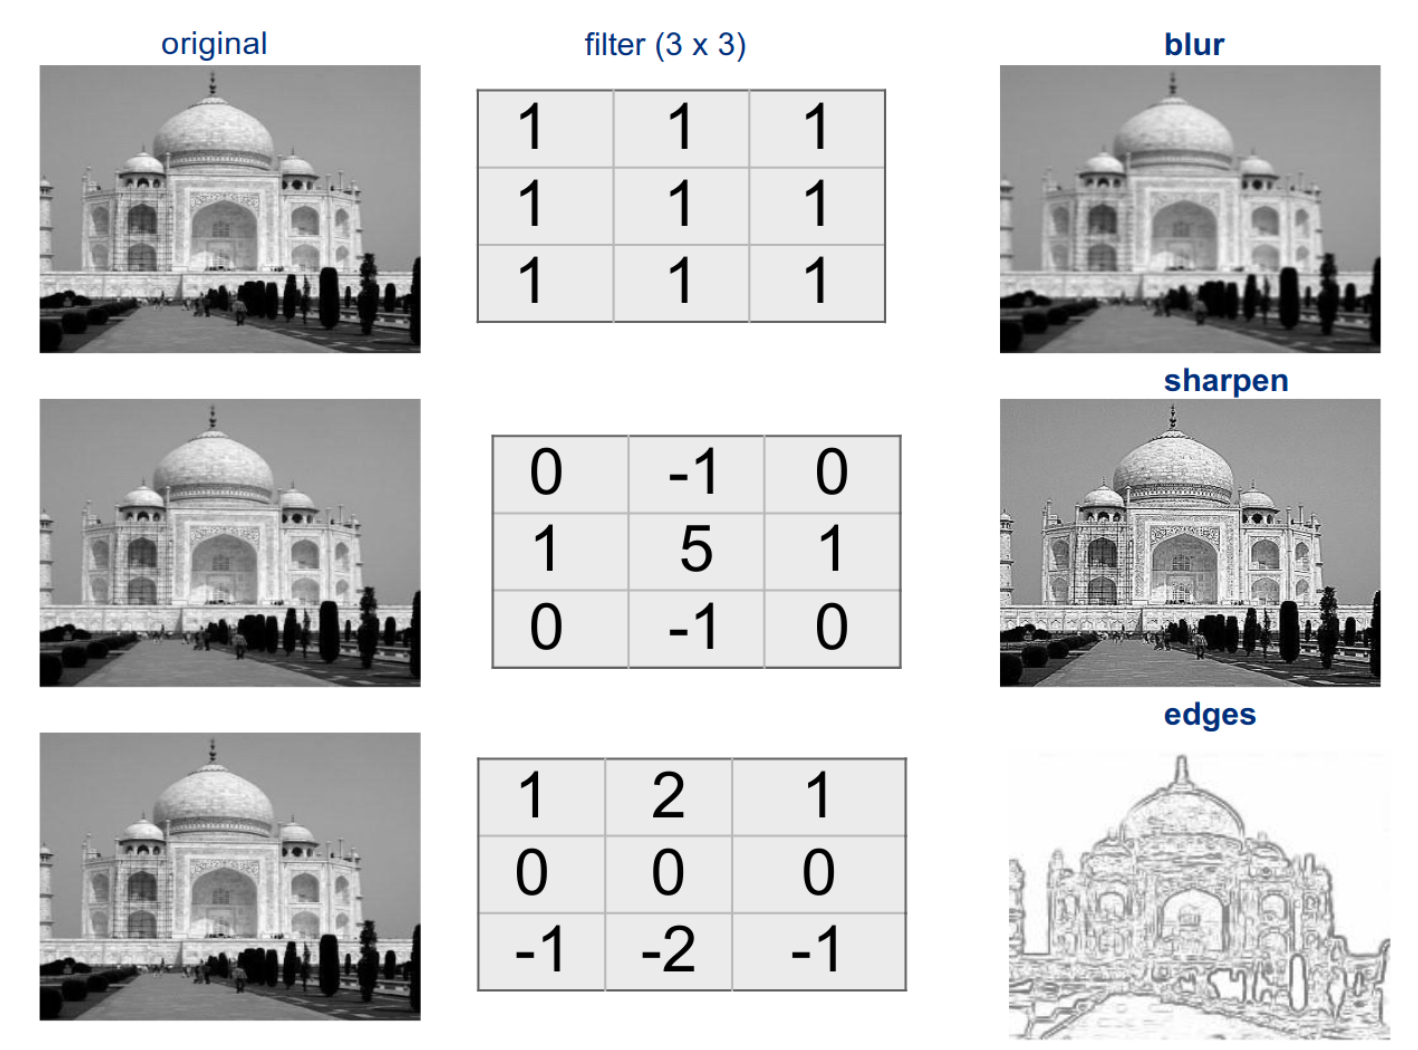
\includegraphics[width=0.75\linewidth]{img/kernels.png}
    
\end{figure}


\begin{definitionbox}{Convolutional Layer}

The convolutional layer is the core building block of a Convolutional Neural Network (CNN). It applies a set of learnable filters to the input data to create feature maps that capture spatial hierarchies of features.

\subsection{Convolution Operation}

Each filter in a convolutional layer has a receptive field, which is the size of the filter or kernel. This field determines the extent of the area in the input data over which the filter is applied.

\begin{itemize}
    \item The output of a filter, the result of a convolution, is a feature map.
    \item A layer can be formed from several channels. Typically there are many filters and feature maps for the same input, with an RGB image having three channels.
    \item Thus, filters or kernels are multi-dimensional tensors as well.
\end{itemize}

The convolution operation is applied across all channels of the input:

\[
\sum_{m}\sum_{n}\sum_{c} x(i + m, j + n, c) F(m, n, c)
\]

where \( x \) represents the input data, \( F \) represents the filter, \( i \) and \( j \) are spatial indices, and \( c \) is the index over the channels.

\subsection{Bias and Activation}

After the convolution operation, a bias term is usually added to the resulting feature map. This bias term is shared across the entire feature map. The final step in the convolutional layer is the application of an activation function to introduce non-linearity into the model:

\[
\theta\left(\sum_{m}\sum_{n}\sum_{c} x(i + m, j + n, c) F(m, n, c) + b\right)
\]

where \( b \) represents the shared bias. \\

The convolutional layers are stacked together, with each layer learning increasingly complex features. The combination of convolution, bias addition, and non-linear activation forms the fundamental components of feature learning in CNNs.

\end{definitionbox}

\section{Strides}
Strides refer to the step of the shift when applying the filter. The most use stride is \(1 \times 1\) stride that shifts a filter by one pixel at a time.\\

Note that for a \( 2 \times 2\) stride, each pixel is only ran through a filter once, so one path is skipped both horizontally and vertically. 

\begin{figure}[H]
    \centering
    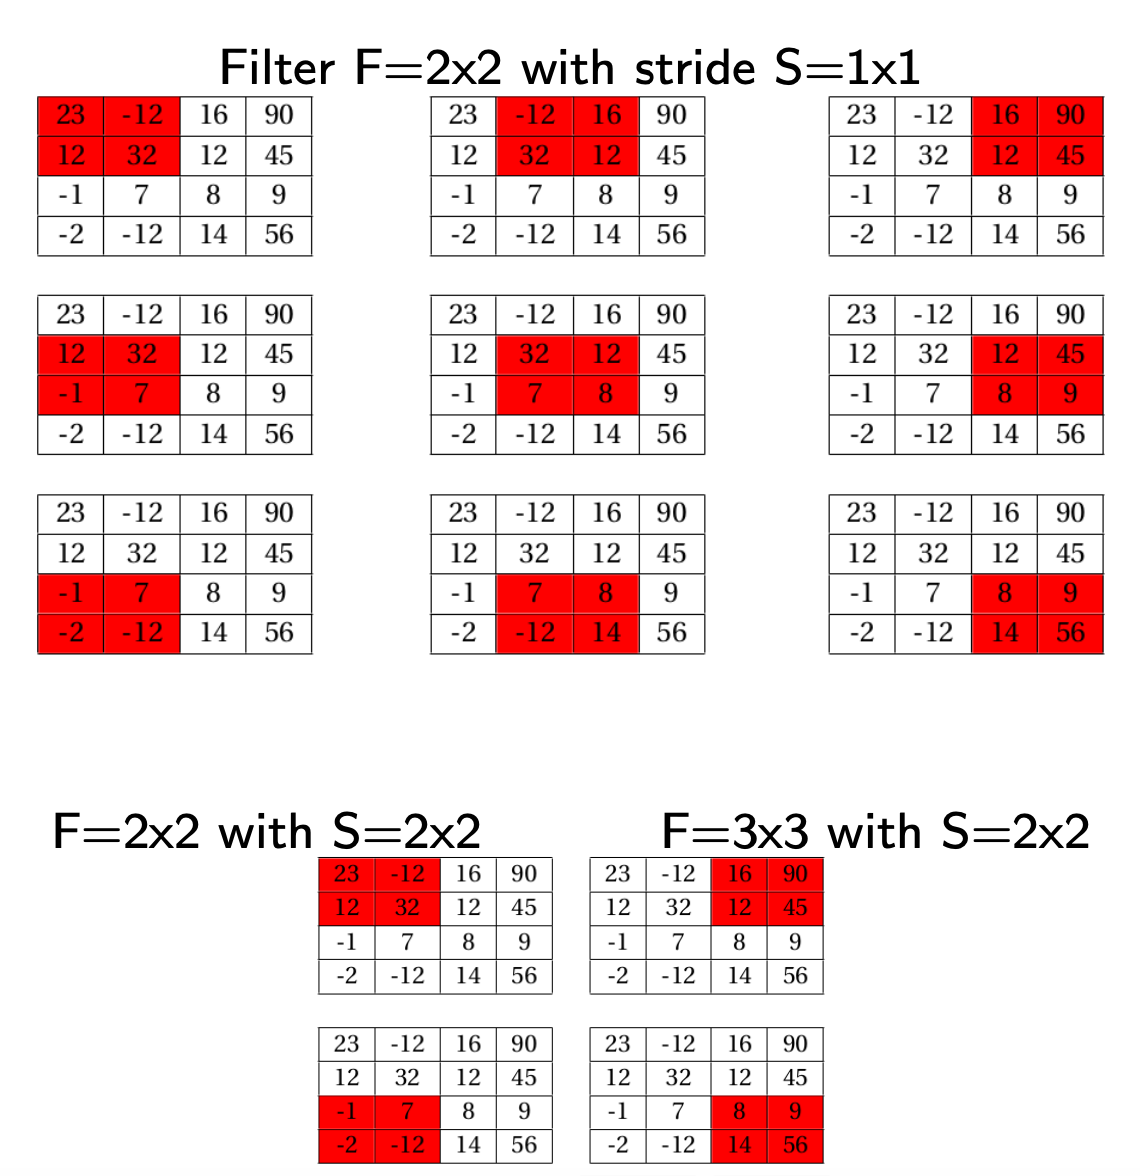
\includegraphics[width=0.75\linewidth]{img/strides.png}
    \caption{Different illustrations of strides for a given image input}
    
\end{figure}

\section{Padding}
Notice that applying the kernel map to the input feature map will result in a smaller output feature map size. This also results in information loss near the borders of the image input map. Some of the naming follows  the \texttt{tensorflow} library.

\begin{itemize}
    \item Note that $K$ refers to the size of the kernel(filter).
    \item VALID padding leaves the input feature map unchanged
    \item SAME padding adds $P=K-1$ zeroes to the input to constrain the output size to be the same for the unit strides. For odd-sized kernels, $P=\lfloor K/2\rfloor $ zeroes are added. So the heights of the input and output are the same, $H_o = H_i$
    \item Full padding adds $P=2(K-1)$ zeroes to the input, with $K-1$ zeroes on both sides. The output height $H_o$ is equal to the input height $H_i$ plus $2(K-1)$. So $H_o = H_i + 2(k-1)$

    
\end{itemize}

The output size for a given padding amount is computed by:

\[
H_o = H_i - K + 2P + 1
\]

Where \(P\) is the padding value.\\

When considering strides, the formula is:

\[
H_o = \frac{H_i - K + 2P}{S} + 1
\]

Where \(S\) is the stride value.

\begin{figure}[H]
    \centering
    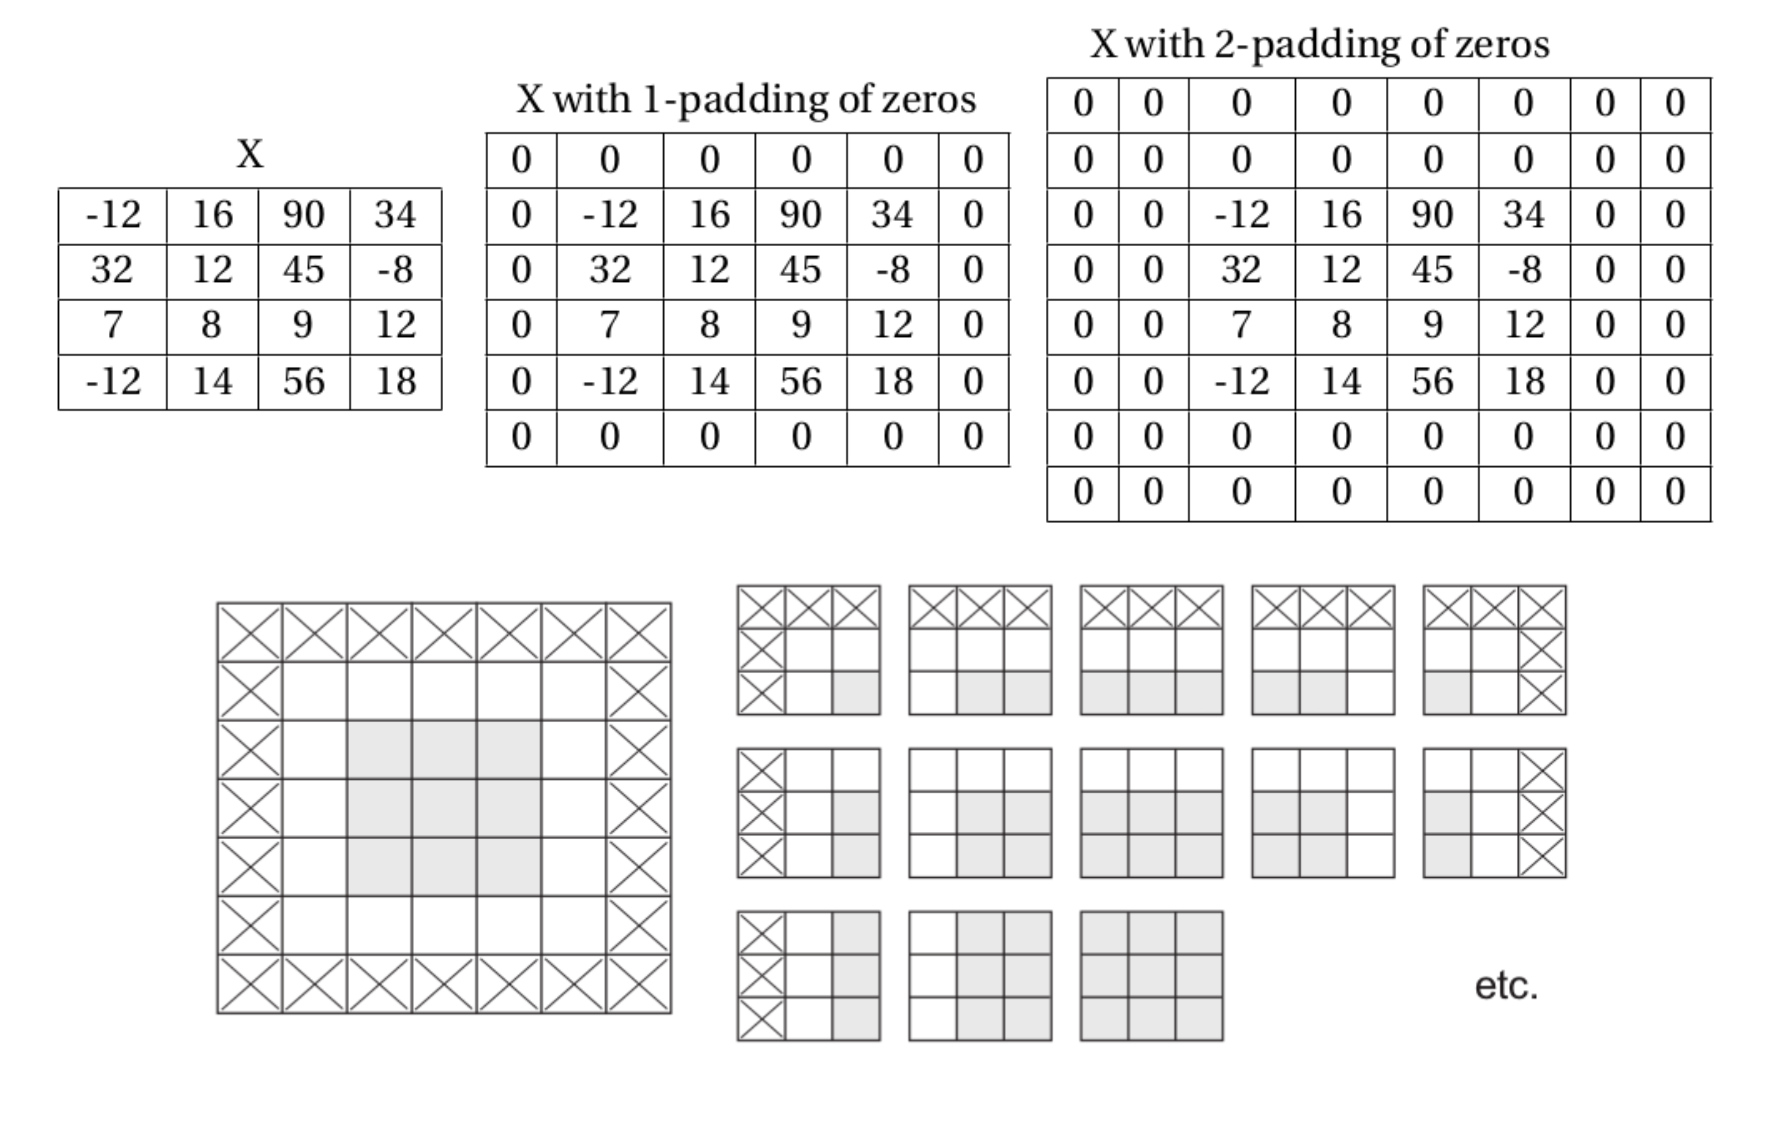
\includegraphics[width=0.75\linewidth]{img/padding.png}
    \caption{Visualisation of different padding levels. Note that to achieve SAME padding for the unlabelled example below, there must be a padding of 2 zeroes thick.}
    
\end{figure}

\section{CNN Properties}
\subsection{CNN Properties Overview}

\begin{itemize}
    \item \textbf{Sparse Connectivity:} Neurons in a CNN layer are connected only to a small region of the layer before it. A small visual field (receptive field) provides enough local information for feature extraction.
    \item \textbf{Shared Weights:} CNNs use the same filter (set of weights) for each position in the input volume, greatly reduces the number of parameters and complexity.
    \item \textbf{Translational Invariance:} Once a feature is learned, the network can recognise it in any other location of the input, although cannot handle rotation or scaling of the feature.
    \item \textbf{Local Correlation:} CNNs take advantage of the fact that nearby pixels in an image are more likely to be correlated, forming recognisable patterns.
    \item \textbf{Flexibility in Input Size:} CNNs can handle inputs of varying sizes for all sizes of images
    \item \textbf{Hierarchical Structure:} The layers of a CNN have the capability to act as a sequence of increasingly complex pattern detectors. Early layers may detect simple edges or textures, while deeper layers can detect more complex structures, such as parts of objects, and even more comprehensive layers can recognise whole objects or scenes.

\begin{figure}[H]
    \centering
    \begin{subfigure}[b]{0.45\linewidth}
        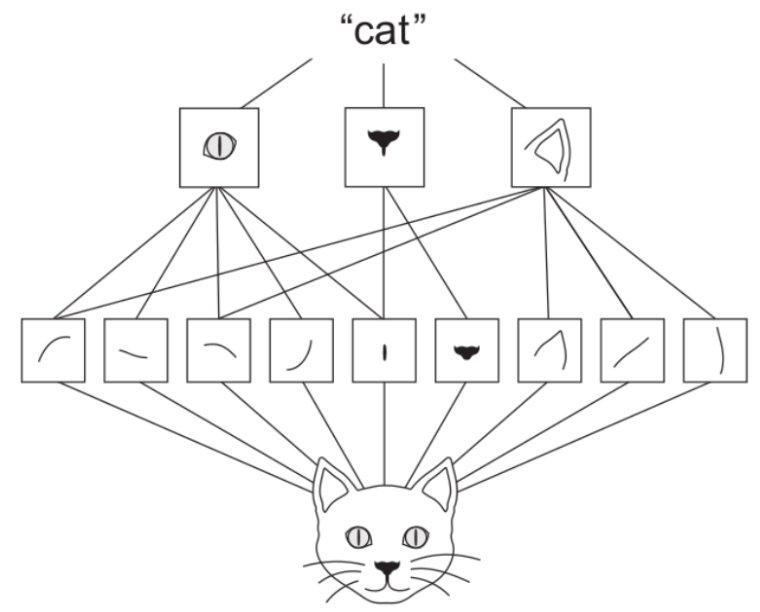
\includegraphics[width=\linewidth]{img/hierarchical_cat.png}
        \caption{Different layers help break down feature detection and selection as hierarchies.}
    \end{subfigure}
    \hfill % optional; add some horizontal spacing
    \begin{subfigure}[b]{0.45\linewidth}
        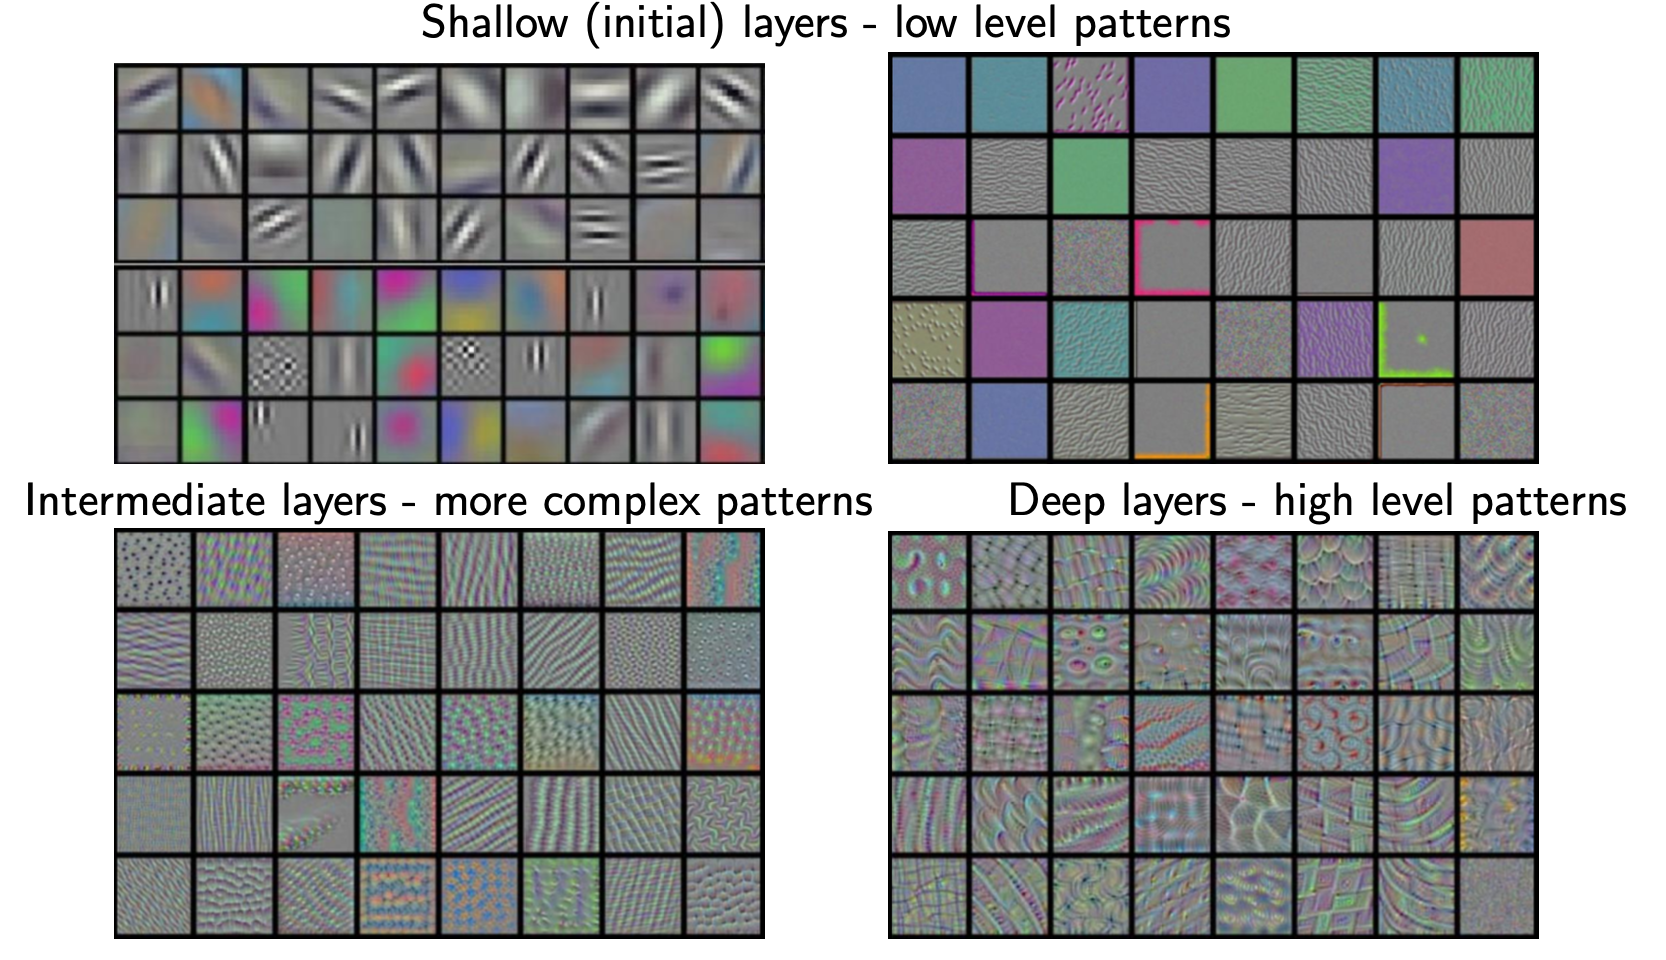
\includegraphics[width=\linewidth]{img/shallow_deep.png}
        \caption{A comparison between shallow and deep networks in terms of feature representation.}
    \end{subfigure}
    \caption{Visualization of hierarchical feature detection in CNNs and the impact of network depth.}
\end{figure}

\end{itemize}

\subsection{CNN Layer Parameters}

The functioning of a CNN is defined by its layer parameters, which dictate how the filters are applied to the input data.

\begin{figure}[H]
    \centering
    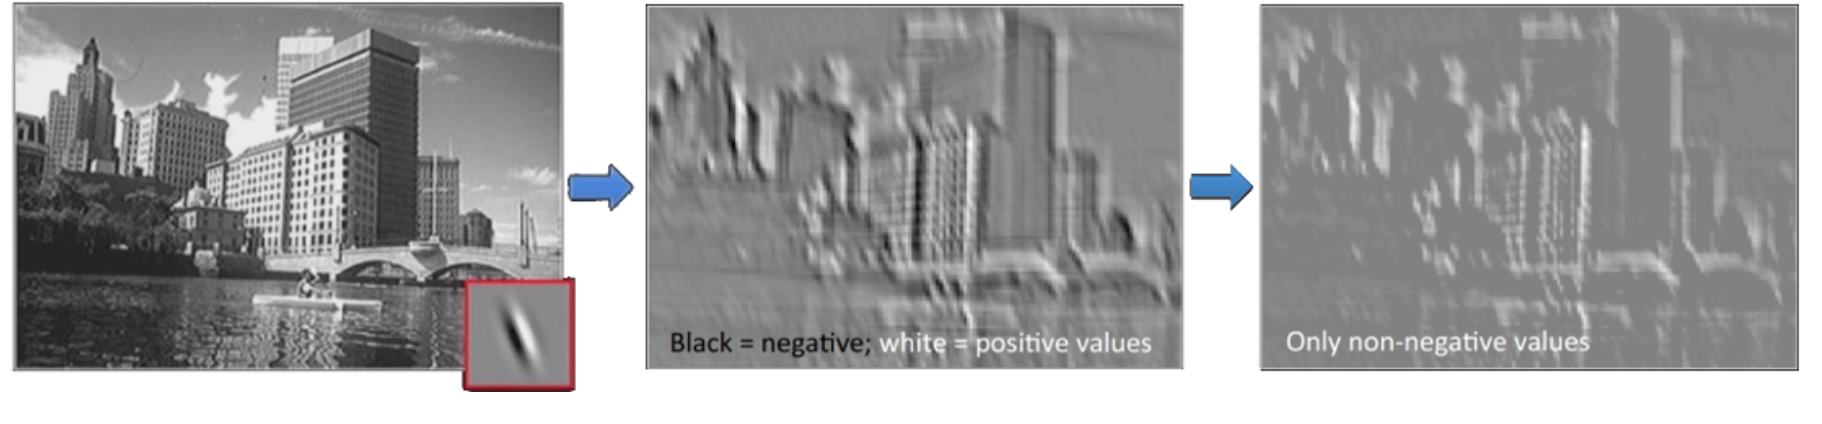
\includegraphics[width=0.75\linewidth]{img/filter_example.png}
    \caption{Filter output and ReLU example}
    
\end{figure}

\begin{itemize}
    \item \textbf{Input:} The input to a convolutional layer is a 3D volume of size \( H_i \times W_i \times D_i \), where \( H_i \) is the height, \( W_i \) is the width, and \( D_i \) is the depth.
    \item \textbf{Parameters:}
    \begin{itemize}
        \item Number of filters \( K \),
        \item Spatial extent of the filter \( F \),
        \item Stride \( S \),
        \item Zero-padding \( P \).
    \end{itemize}
    \item \textbf{Output:} The output is also a 3D volume with dimensions \( H_o \times W_o \times D_o \), given by:
    \begin{itemize}
        \item \( W_o = \frac{W_i - F + 2P}{S} + 1 \),
        \item \( H_o = \frac{H_i - F + 2P}{S} + 1 \),
       
        \item \( D_o = K \).
    \end{itemize}
    \item With \textbf{parameter sharing}, each filter has \( F \cdot F \cdot D_i \) weights, resulting in a total of \( F \cdot F \cdot D_i \cdot K \) weights and \( K \) biases for the layer.
    \item \textbf{Common Settings:} Typically, filters have sizes like \( F \in \{ 2,3,4 \ldots 15\} \), with stride \( S = 1 \) or \( 2 \) and padding \( P  = 0\). Padding can be modified if the post-convolution image needs a different resolution.
    \item In the \textbf{output volume}, the \( d \)-th depth slice (size \( W_o \times H_o \)) corresponds to the activations of the \( d \)-th filter applied at every position of the input, taking stride \( S \) into account and adding the \( d \)-th bias.
\end{itemize}


\section{Pooling Methods}

The pooling layer performs non-linear downsampling via a sliding window across the feature map.It aggregates information from the feature maps obtained from the convolutional layers, and reduces their spatial dimensions while retaining the most important information.\\

A pooling function replaces the output of the network at a certain location with a summary statistic of the nearby outputs– it discards information in the process. For instance, max pooling returns the maximum output within a local region of inputs.\\

This helps reduce the dimensions of data. Common pooling functions include max pooling and average pooling.

\begin{itemize}
    \item \textbf{Max Pooling:} Typically involves \( 2 \times 2 \) filters with a stride of 2, discarding 75\% of the activations. This downsampling reduces each spatial dimension by half, preserving the depth dimension.
    \item \textbf{Average Pooling and L2-Norm Pooling:} These are alternative pooling methods that compute the average and L2 norm of the pooling region, respectively.
\end{itemize}



\begin{figure}[H]
    \centering
    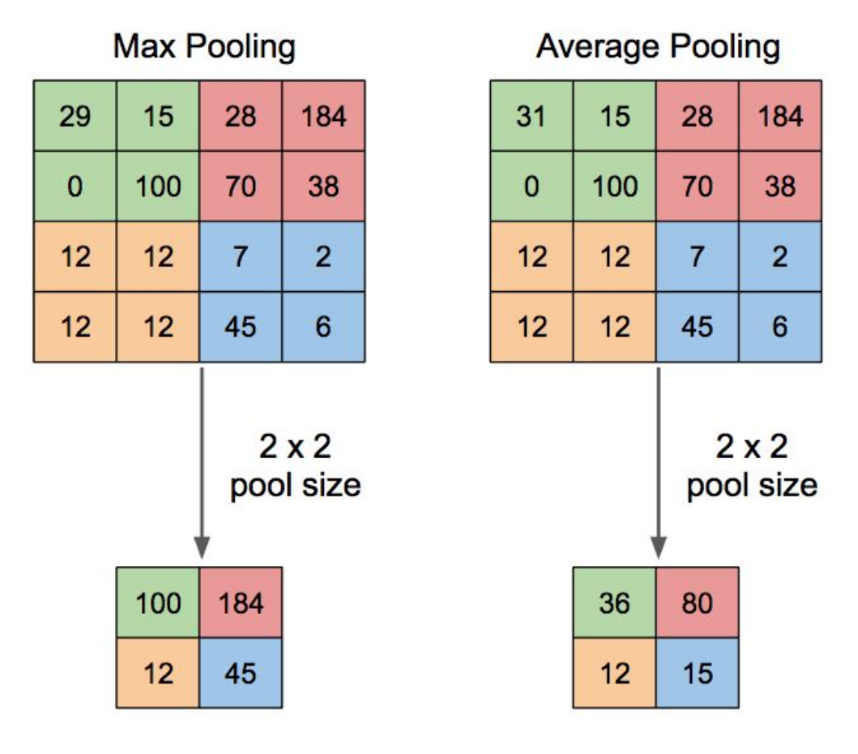
\includegraphics[width=0.4\linewidth]{img/pooling.png}
    
    
\end{figure}

\subsection{Mathematical Description}

Consider a feature map represented by \( A \) where the pooling operation is applied. For a \( 2 \times 2 \) pooling region with stride 2, the max pooling operation can be described as:

\[
Z_{ij} = \max(A_{2i:2i+1, 2j:2j+1})
\]

and for average pooling:

\[
Z_{ij} = \frac{1}{4} \sum_{m=2i}^{2i+1} \sum_{n=2j}^{2j+1} A_{mn}
\]

where \( Z \) is the resulting feature map after pooling, and \( A_{mn} \) denotes the activation in the \( m \)-th row and \( n \)-th column of the feature map \( A \).



The pooling layer operates on the feature maps to perform downsampling, effectively reducing the spatial dimensions while preserving the depth.

\subsubsection{Input and Output Dimensions}

Given an input volume of size \( H_i \times W_i \times D_i \), the output volume \( H_o \times W_o \times D_o \) after the pooling operation is determined by:

\begin{itemize}
    \item \textbf{Spatial Extent \( F \)}: The size of the filter, typically \( F \in \{2, \ldots, 4\} \).
    \item \textbf{Stride \( S \)}: The step size with which the filter moves across the input volume, commonly \( S = 2 \).
    \item \textbf{Padding \( P \)}: Usually set to 0 in pooling layers.
    \item The output dimensions are calculated as:
    \begin{align*}
        W_o &= \frac{W_i - F}{S} + 1, \\
        H_o &= \frac{H_i - F}{S} + 1, \\
        D_o &= D_i.
    \end{align*}
    \item This results in a reduction of the spatial dimensions of the input, with the depth remaining unchanged.
\end{itemize}

\subsubsection{Characteristics of Pooling Layers}


\begin{figure}[H]
    \centering
    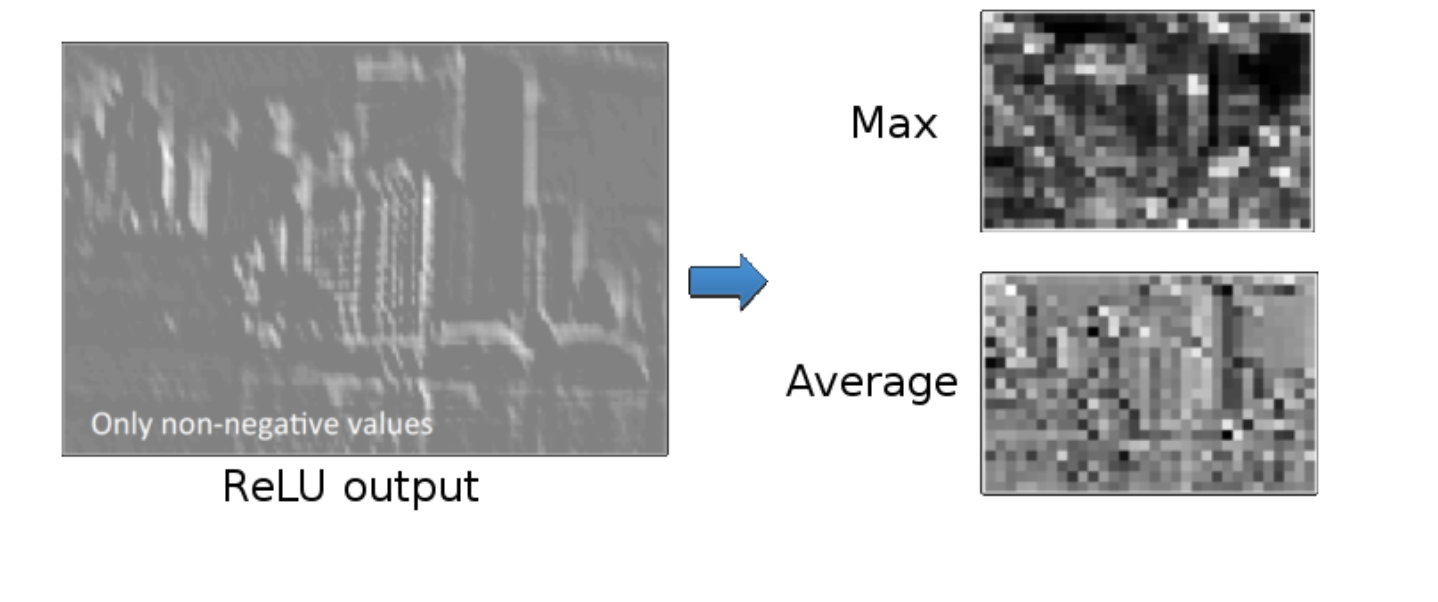
\includegraphics[width=0.5\linewidth]{img/max_avg_pool.png}
    
    
\end{figure}

\subsection{Properties of Pooling Layers}

\begin{itemize}
    \item \textbf{Dimensionality Reduction:} Pooling layers decrease the height and width of the input volume, which reduces the computational load for the subsequent layers.
    \item \textbf{Translational Invariance:} Pooling operations help the network to achieve translational invariance, meaning that shifting the input by a small amount will not change the output of the pooling layer significantly. This makes the CNN less sensitive to the exact spatial locations of features within the input volume.
    \item \textbf{Reduced Sensitivity:} By downsampling, the network becomes less sensitive to the exact location of features in the input space, which contributes to the generalisation capabilities of the network.
    \item \textbf{Efficiency:} Pooling layers reduce the computational load for subsequent layers by decreasing the number of parameters and computations.
    \item \textbf{No Learnable Parameters:} Unlike convolutional layers, pooling layers do not have weights or biases to learn. The pooling operation is deterministic and based solely on the predefined operation, such as max or average pooling.
    \item \textbf{Zero Padding:} Pooling layers typically do not use zero-padding as their primary goal is to reduce dimensionality rather than preserve it.
    \item \textbf{Handling of Varying Input Sizes:} The down-sampling nature of pooling allows CNNs to handle inputs of varying sizes effectively.
\end{itemize}

\subsection{Gradient Propagation}

During backpropagation, the gradient is only passed through the locations that contributed to the maximum in the case of max pooling:

\[
\frac{\partial Z_{ij}}{\partial A_{mn}} = 
\begin{cases} 
1 & \text{if } A_{mn} \text{ is the max value} \\
0 & \text{otherwise}
\end{cases}
\]

For average pooling, the gradient is distributed equally among all the elements of the pooling region.


\section{Fully Connected Layer in CNNs}

The Fully Connected (FC) layer, often found at the end of Convolutional Neural Networks, performs classification tasks by synthesising the features extracted by previous layers to form the final output.

\subsection*{Characteristics of the Fully Connected Layer}

\begin{itemize}
    \item It operates on a flattened input where all the spatial information is converted into a single vector of neurons.
    \item Each neuron in a fully connected layer is connected to all activations in the previous layer, resulting 
    \item It is the final learning phase that maps the extracted features to the desired outputs.
    \item The layer's adaptability makes it suitable for both classification and encoding tasks.
\end{itemize}

\subsection*{Mathematical Formalism}

The operations within a Fully Connected layer can be described mathematically as follows:\\

Given an input feature map $F \in \mathbb{R}^{h \times w \times d}$, where $h$, $w$, and $d$ represent height, width, and depth respectively, the feature map is flattened into a vector $v \in \mathbb{R}^{hwd}$.\\

This vector is then transformed by the FC layer using a weight matrix $W \in \mathbb{R}^{n \times hwd}$ and a bias vector $b \in \mathbb{R}^{n}$, with $n$ being the number of neurons in the FC layer. The output $o \in \mathbb{R}^{n}$ of the FC layer is given by:

\begin{equation}
o = \sigma(Wv + b)
\end{equation}

where $\sigma$ denotes the activation function, which can be a sigmoid, softmax, or any other non-linear function. In the context of classification, the softmax function is commonly used to convert the output into probability distributions:

\begin{equation}
\text{Softmax}(o_i) = \frac{e^{o_i}}{\sum_{j=1}^{n} e^{o_j}} \quad \text{for } i=1,2,\ldots,n
\end{equation}

\subsection*{Sequence in CNNs}

The typical sequence of operations in a CNN before reaching the FC layer is:

\begin{enumerate}
\item \textbf{Convolution:} Extracts features by applying filters to the input.
\item \textbf{Pooling:} Reduces the spatial size of the representation, decreasing the number of parameters and computation in the network.
\item \textbf{Flattening:} Transforms the 2D feature maps into a 1D feature vector.
\item \textbf{Fully Connected Layer:} Utilises the flattened vector for classification or regression tasks.
\end{enumerate}

\begin{figure}
    \centering
    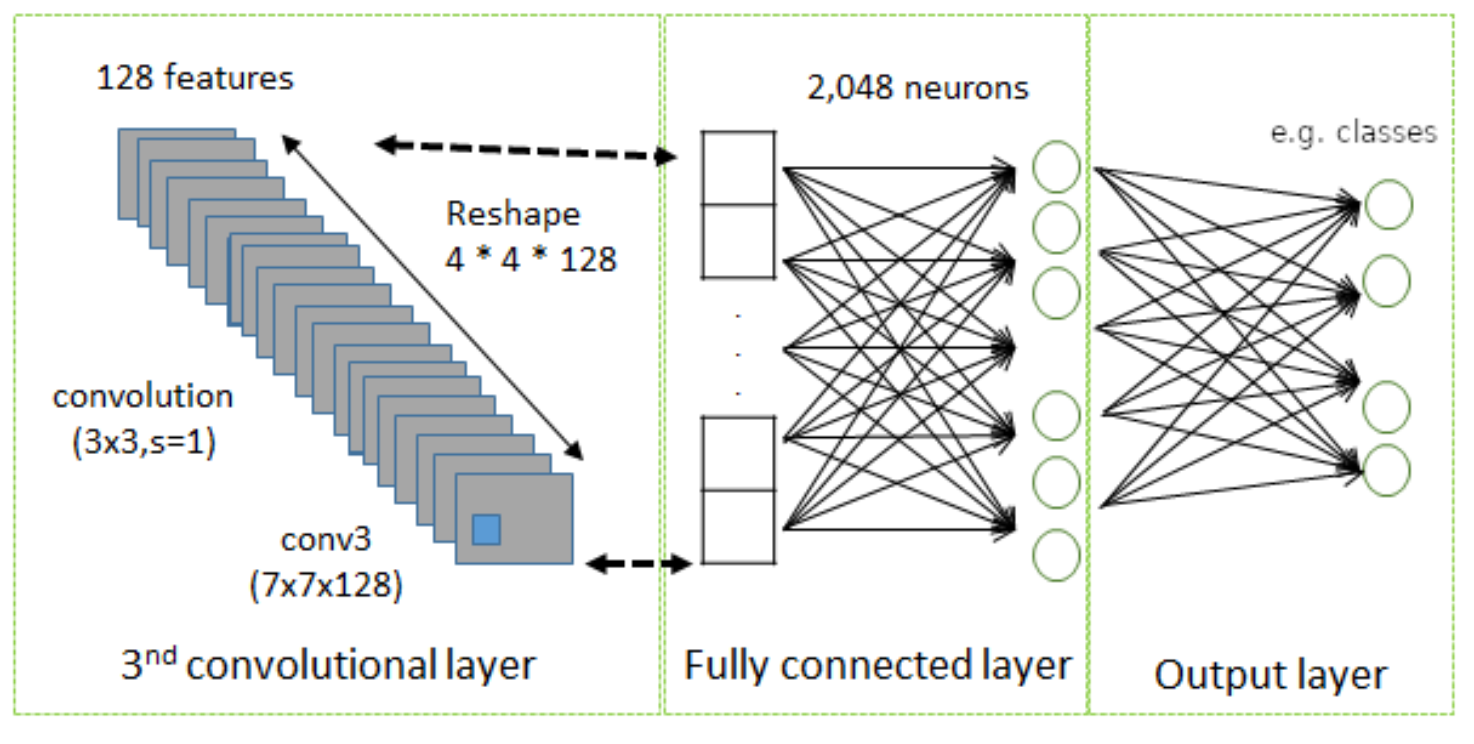
\includegraphics[width=0.75\linewidth]{img/FC.png}
    \caption{Visualisation of the FC Layer} 
\end{figure}

\section{Loss Layer}
\begin{itemize}
    \item The loss layer is required for training the network.
    \item Input: It takes in network predictions and the ground truth, which are samples of the target function.
    \item Output: the prediction error as a scalar
    \item The Loss function can be set depending on the task and data. 
    \item For classification, the softmax (sigmoid) activation function is used followed by cross-entropy loss.
    \item For regression, L1, L2, and Smooth L2 losses are used.
\end{itemize}

\subsection*{Loss Layer for Binary Classification}

Binary classification in CNNs can be thought of as a decision-making process, where the network learns to differentiate between two distinct classes (e.g., 'dog' vs 'no dog'). The sigmoid function squashes the output of the linear combination of inputs and weights into a range between 0 and 1, giving us a probability score. The cross-entropy loss then quantifies the difference between the predicted probability and the actual class. A lower loss indicates better model performance, implying that the predicted probability is closer to the actual class label.


\begin{figure}[H]
    \centering
    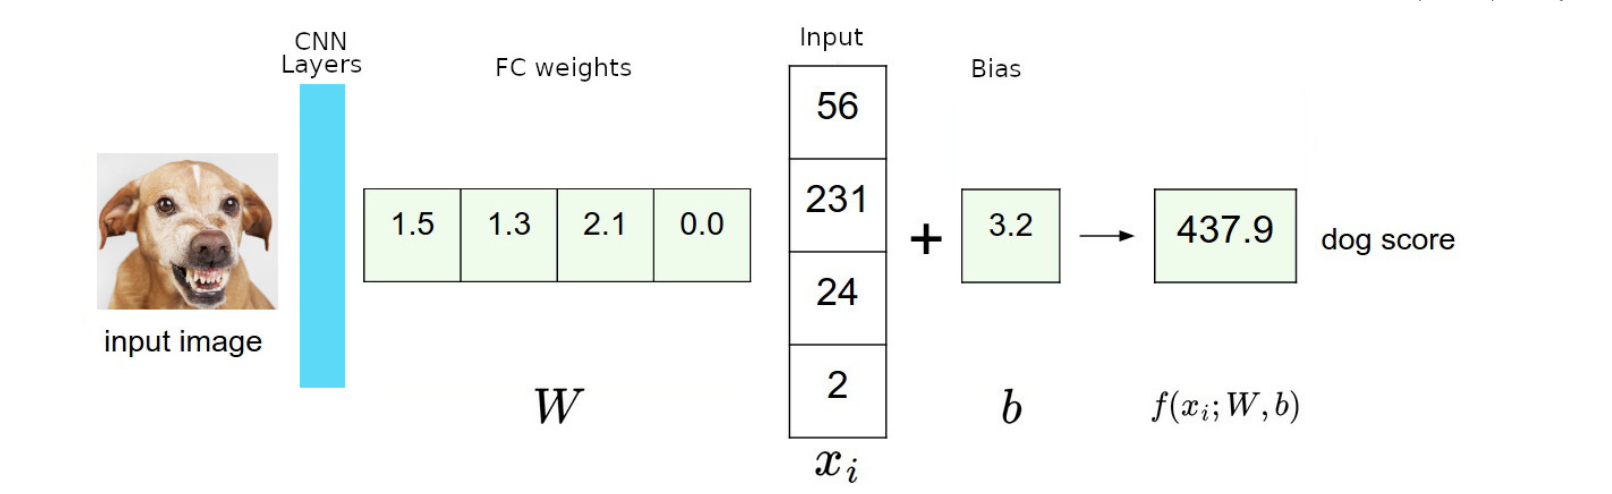
\includegraphics[width=0.6\linewidth]{img/dogloss.png}
    \caption{Graphical representation of Log Loss when the true label is 1.}
\end{figure}


\begin{itemize}
    \item Given a ground truth label \( y \) and a network prediction \( \hat{y} \), where \( y \in \{0,1\} \) and \( \hat{y} \) is the sigmoid activation function applied to the linear combination of inputs and weights:
    \[ \hat{y} = \frac{e^{W^Tx+b}}{e^{W^Tx+b}+1} \]
    \item This formulation allows \( \hat{y} \) to be interpreted as the probability of the input being classified as class 1 (for example, detecting if an image contains a dog).
    
    \item The \textbf{Cross-entropy loss function} \( \mathcal{L} \) is defined as:
    \[ \mathcal{L} = -y \log(\hat{y}) - (1-y) \log(1-\hat{y}) \]
    This function penalises the deviation of \( \hat{y} \) from the true label \( y \). It is particularly sensitive to confident but incorrect predictions, which is desirable in a loss function.
\end{itemize}



For an input image classified with a high confidence (\( \hat{y} \approx 1 \)), and the true label being 1 (indicating presence of a dog), the loss is close to 0 as seen in the function:
\[ \mathcal{L} = -1 \log(1) + (1-1) \log(1 - \hat{y}) = 0 \]

Note that \( \hat{y} \) as a probability is never exactly 0 or 1 but always in between, reflecting a degree of uncertainty.

\subsection*{Loss Layer for Multiclass Classification}

Multiclass classification is akin to a voting system where each class competes for the highest probability score. The Softmax function acts like a normaliser, converting raw scores (logits) into probabilities that sum up to one. The cross-entropy loss then measures how well the predicted probability distribution aligns with the actual distribution (the ground truth). 



\begin{itemize}
    \item For a multi-label ground truth vector \( \mathbf{y} \) and a prediction vector \( \hat{\mathbf{y}} \in \mathbb{R}^K \), where \( K \) is the number of classes, the model uses the \textbf{Softmax} function for the prediction:
    \[ \hat{y}_k = \frac{e^{W_k^T\mathbf{x}+b}}{\sum_{i}e^{W_i^T\mathbf{x}+b}} \]
    \item The \textbf{Categorical (multiclass) cross entropy error} \( \mathcal{L} \) for each class \( k \) is computed as:
    \[ \mathcal{L}_k = -y_k \log(\hat{y}_k) \]
    This error is summed or averaged over all classes to provide a total loss for a single prediction.
    
    \item It is often noted that this method is \textbf{superior to classification error or Mean Squared Error (MSE)}:
    \begin{itemize}
        \item \textit Classification error ignores the confidence of the predictions.
        \item MSE places too much emphasis on incorrect outputs, which can lead to poor performance in classification tasks.
    \end{itemize}
\end{itemize}


\begin{figure}[H]
    \centering
    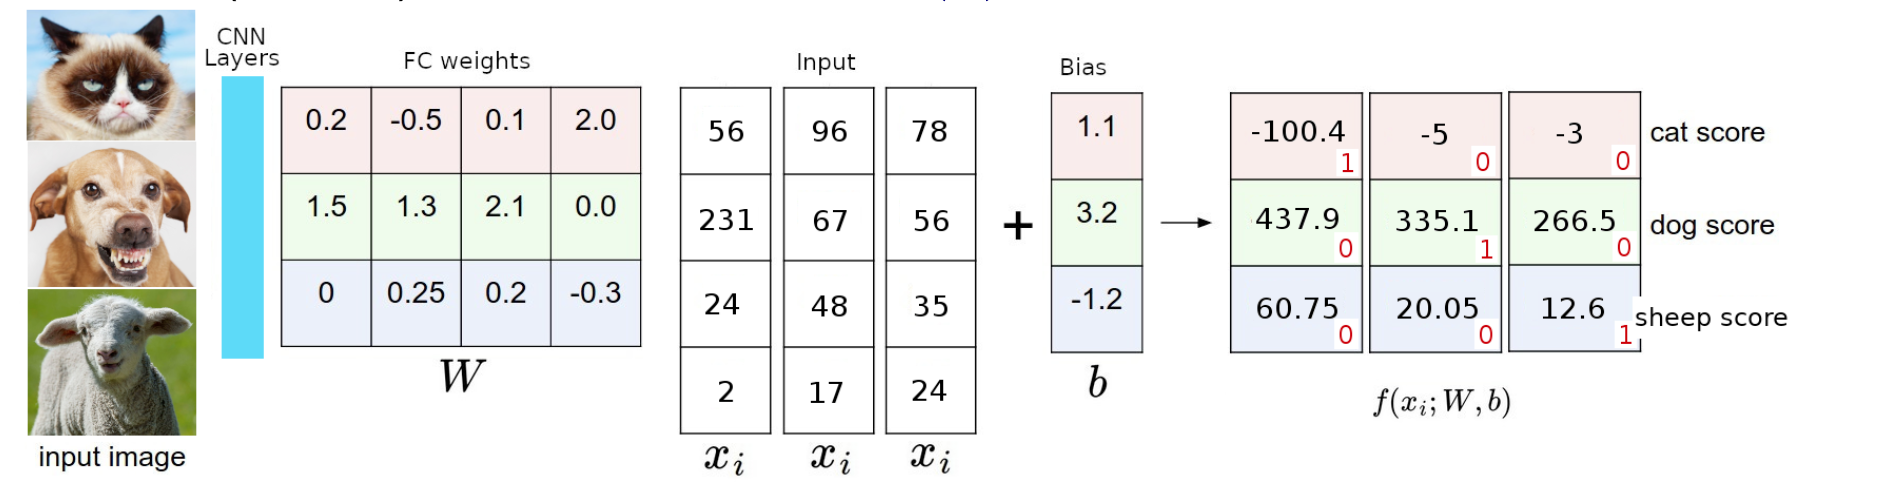
\includegraphics[width=0.85\linewidth]{img/animals.png}
    \caption{Diagram of a categorical (multiclass) loss layer. Note that one image is sent as an input.}
    
\end{figure}

\subsubsection*{Average Cross Entropy Loss Calculation Example}
For an example with three classes, represented as `cat`, `dog`, and `sheep`, the average cross entropy (ACE) loss \( \mathcal{L} \) would be calculated for a single instance as:
\[ \mathcal{L} = \frac{1}{3} \left( -y_{1} \log(\hat{y}_{1}) + -y_{2} \log(\hat{y}_{2}) + -y_{3} \log(\hat{y}_{3}) \right) \]

So the cat score \(\hat{y}_{1,1}=\frac{e^{-100.4}}{e^{-100.4}+e^{437.9}+e^{60.75}}\)

\subsubsection*{Hinge loss comparison}

\[\mathcal{L}=\sum_{j\neq k}\max(0,\hat{y}_j-\hat{y}_k+1)\]

The hinge loss calculation is the sum of the differences between the score for the non-correct classes and the score for the correct class (plus the margin), but only when those differences are positive.

This is typically used with Support Vector Machine (SVM) models.



\begin{figure}[H]
    \centering
    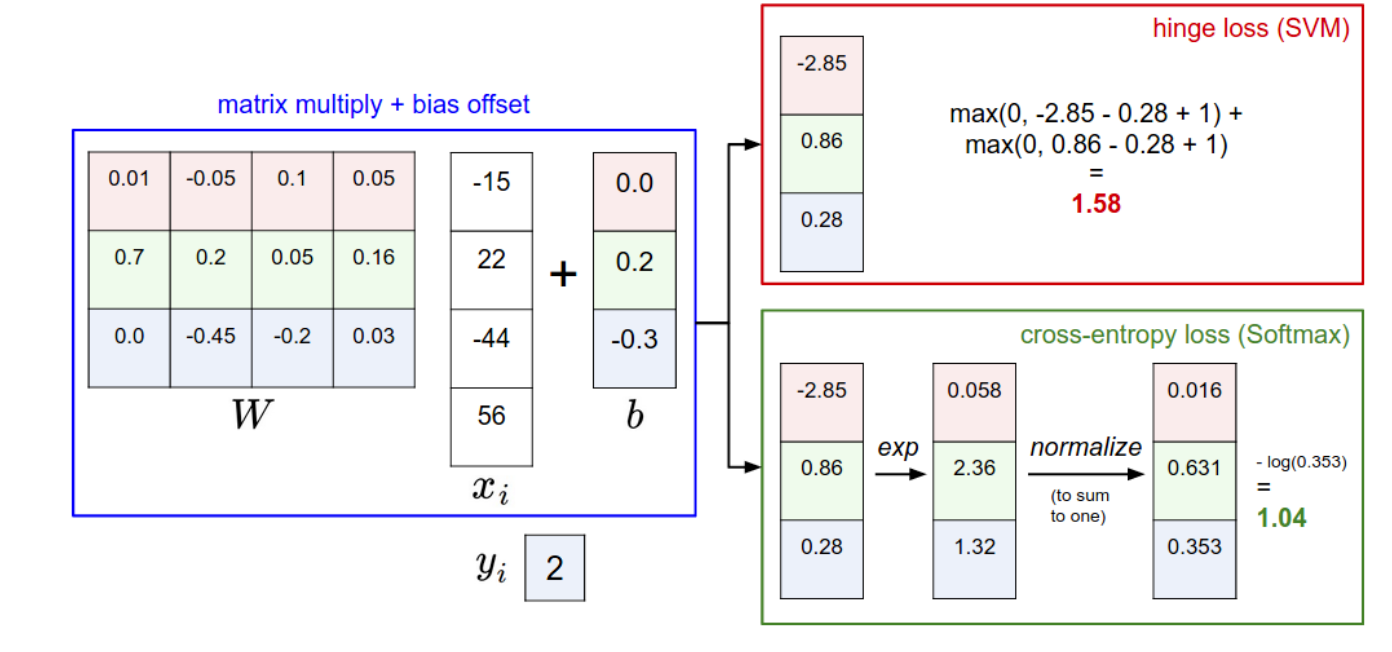
\includegraphics[width=1\linewidth]{img/hinge_softmax.png}
    \caption{Comparison of layers for of Cross Entropy Loss vs Hinge Loss}
    \label{fig:enter-label}
\end{figure}

\section{Loss Layer for Regression}

In regression tasks within machine learning, the goal is to predict continuous values, and the loss layer is responsible for measuring the discrepancy between the predicted values \( \hat{y} \) and the actual ground truth values \( y \).

\begin{itemize}
    \item The \textbf{L2 Loss} or \textbf{Mean Squared Error (MSE)} is the square of the Euclidean distance between the network's prediction and the true value:
    \[ \mathcal{L}_2 = \lVert wx + b - y \rVert^2 = (wx + b - y)^2 \]
    \[ \text{MSE} = \frac{1}{N} \sum_{i=1}^{N} \mathcal{L}_2(i) \]
    where \( N \) is the number of samples.

    \item The \textbf{L1 Loss} or \textbf{Mean Absolute Error (MAE)} measures the absolute difference:
    \[ \mathcal{L}_1 = \lvert wx + b - y \rvert \]
    \[ \text{MAE} = \frac{1}{N} \sum_{i=1}^{N} \mathcal{L}_1(i) \]

    \item \textbf{Smooth L1 Loss} (also known as Huber loss) is a combination of L1 and L2 losses:
    \[ \mathcal{L}_{\text{smooth}} = \begin{cases} 
    0.5 \times \mathcal{L}_2, & \text{for } \mathcal{L}_1 < 0.5 \\
    \mathcal{L}_1 - 0.5, & \text{otherwise}
    \end{cases} \]
    This loss is less sensitive to outliers than L2 loss.
\end{itemize}

The graph on the slide provides a visual comparison of these loss functions. The L2 loss increases quadratically and is more sensitive to larger errors, while the L1 loss grows linearly. The Smooth L1 Loss combines these two behaviours: it is quadratic for small errors and linear for large errors, which makes it robust to outliers.

\begin{figure}[H]
\centering
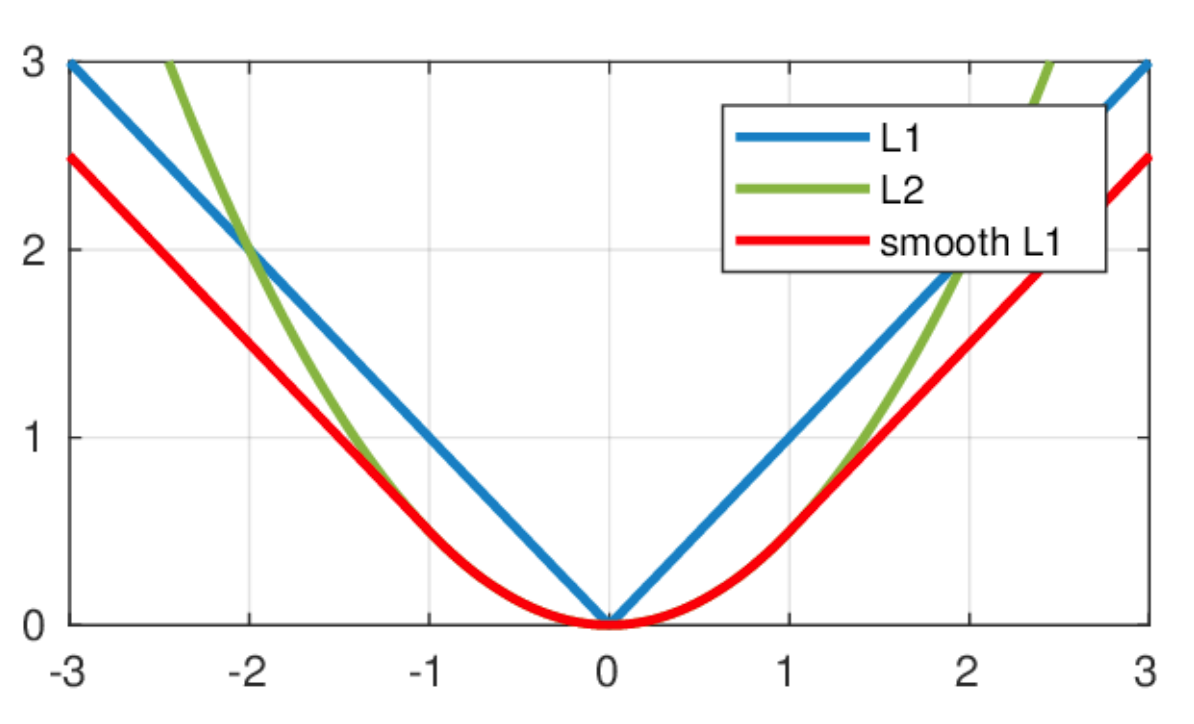
\includegraphics[width=0.5\textwidth]{img/l1_l2.png}
\caption{Comparative graph of L1, L2, and Smooth L1 Loss functions.}
\end{figure}

In practice, the choice of loss function can significantly affect the regression model's performance, particularly in terms of sensitivity to outliers in the training data.
\begin{figure}[H]
    \centering
    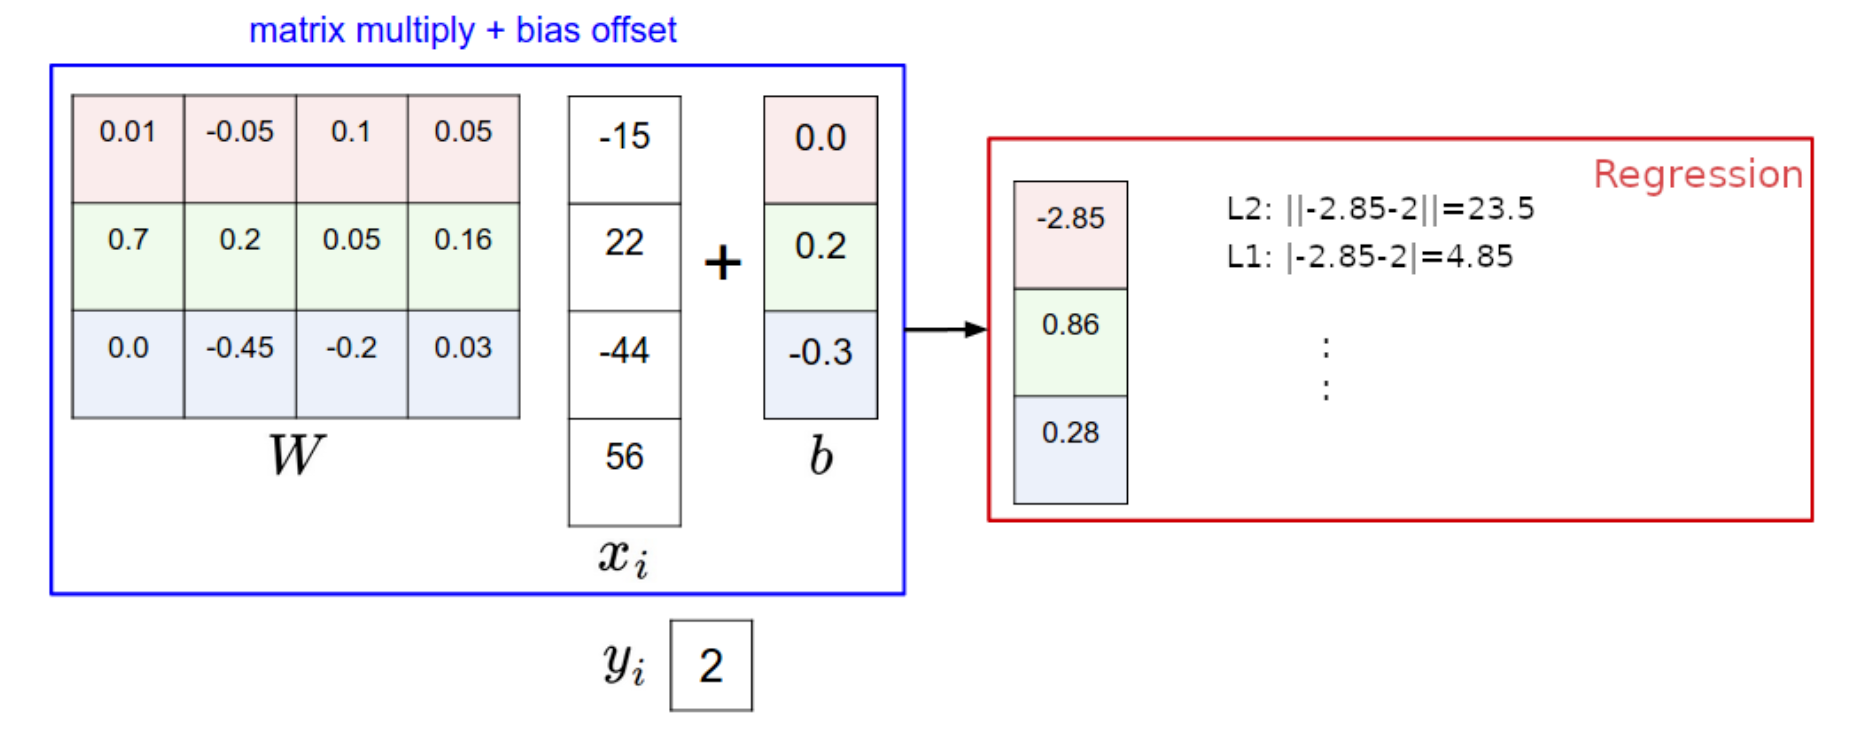
\includegraphics[width=1\linewidth]{img/losslayer-regression.png}
    \caption{Diagram of a categorical (multiclass) regression loss layer }
\end{figure}


\section{Practical Hints for CNNs}

\subsection*{Number of Filters}
\begin{itemize}
    \item The number of filters in a CNN directly influences the network's capacity and its ability to capture features from the input data.
    \item This number should be balanced with the complexity of the task and the volume of available training data.
    \item Computing activations with convolutional operations is more computationally expensive than in Multilayer Perceptrons (MLPs), even though the size of the neuron is smaller.
    \item Typically, initial layers have fewer filters compared to deeper layers. This reflects the progression from capturing basic features to more complex ones.
    \item Adjusting the number of filters can balance the computational load across the network and maintain a consistent level of feature representation at each layer.
\end{itemize}

\subsection*{Filter Shape}
\begin{itemize}
    \item The dimensions of the filters depend on the type of input data and the abstractions that the network needs to learn.
    \item Large filters (e.g., 11x11) are often used in the first layers to capture broad features, while smaller filters (e.g., 5x5) are used in deeper layers for finer details.
\end{itemize}

\subsection*{Pooling}
\begin{itemize}
    \item Pooling layers reduce the spatial dimensions of the feature maps. Typical configurations include 2x2 or no max-pooling.
    \item The trend in deep learning is moving towards using smaller filters and deeper architectures, sometimes foregoing pooling layers to preserve information.
    \item For inputs with large spatial dimensions, larger pooling (e.g., 4x4) might be used, but there is a risk of losing too much detail.
\end{itemize}

\subsection*{Loss Functions}
\begin{itemize}
    \item For classification tasks, the Softmax function is typically used in conjunction with a cross-entropy loss.
    \item In regression tasks, L2 (Mean Squared Error) or Smooth L1 (Huber Loss) are common choices for loss functions.
\end{itemize}

\subsection*{Typical Sequence of Layers in Shallow Networks}
\begin{itemize}
    \item A common architecture sequence for shallow networks is:
    \begin{verbatim}
        INPUT → [CONV → Norm → RELU → POOL] (x2) → FC → RELU → FC → OUTPUT
    \end{verbatim}
    \item Another variant might be:
    \begin{verbatim}
        INPUT → [CONV → RELU → CONV → RELU → POOL] (x3) → [FC → RELU] (x2) → FC → OUTPUT
    \end{verbatim}
\end{itemize}

    
    

\chapter{Network Training}
\section{Backpropagation in Neural Networks}


\begin{figure}[H]
    \centering
    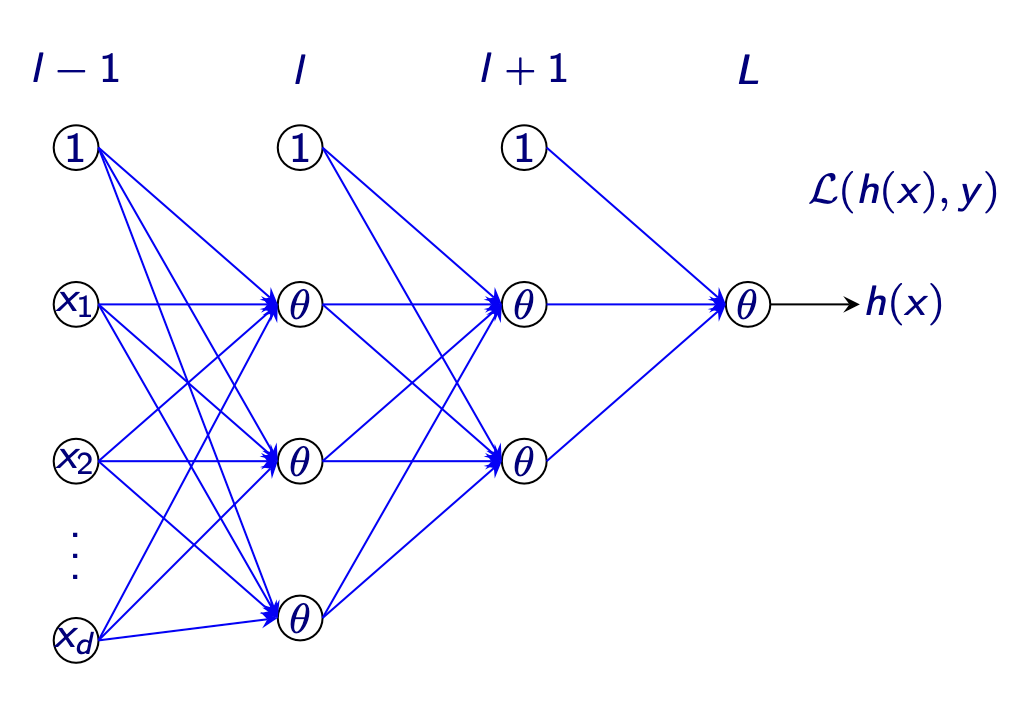
\includegraphics[width=0.55\linewidth]{img/nn.png}
\end{figure}

\begin{itemize}
    \item \textbf{Weights} are denoted as \( W^{(l)} \) for layer \( l \), with \( W_{ij}^{(l)} \) representing the weight from the \( i \)-th neuron in layer \( l-1 \) (input) to the \( j \)-th neuron in layer \( l \) (output). The layer indexing runs from 1 to \( L \) where \( L \) is the total number of layers.
    \item The \textbf{input} vector \( x \) applied to the input layer, represented as \( x^{(0)} \) with components \( x_1^{(0)}, \ldots, x_{d^{(0)}}^{(0)} \), leads to the output \( x_1^{(L)} = h(x) \in \mathbb{R} \), where \( h(x) \) is the hypothesis function.
    \item \textbf{Activations} (outputs) of layer \( l \) are denoted as \( x_j^{(l)} \), which are computed using an activation function \( \theta \) applied to the pre-activation values \( s_j^{(l)} \). This can be expressed as:
    \[ x_j^{(l)} = \theta(s_j^{(l)}) = \theta \left( \sum_{i=0}^{d^{(l-1)}} W_{ij}^{(l)} x_i^{(l-1)} \right) \]
    where \( d^{(l-1)} \) and \( d^{(l)} \) are the number of inputs and outputs for layer \( l \), respectively.
    \item The \textbf{diagonal matrix of activations} at layer \( l \), denoted as \( \Theta^{(l)} \), is the diagonal matrix containing the activation function derivatives and can be calculated as:
    \[ \Theta^{(l)} = \text{diag}(\theta'(s^{(l)})) \]
    which is a square matrix with dimensions equal to the number of outputs of layer \( l \).
    \item The \textbf{gradient} with respect to the pre-activation values \( s^{(l)} \) is given by \( \delta^{(l)} \), which is used in the backpropagation algorithm to compute the gradient of the loss function with respect to the weights \( W^{(l)} \).
\end{itemize}


\begin{definitionbox}{Gradient}
The gradient \( \delta^{(l)} \) for layer \( l \) in a neural network during backpropagation is given by:
\[ \delta^{(l)} = \left( \prod_{k=l}^{L-1} \Theta'(s^{(k)})W^{(k)T} \right)\Theta'(s^{(L)}) \nabla_{x^{(L)}} \mathcal{L} \]
where \( \Theta'(s^{(l)}) \) is the derivative of the activation function evaluated at the pre-activation level \( s^{(l)} \), \( W^{(k)} \) are the weights of layer \( k \), and \( \nabla_{x^{(L)}} \mathcal{L} \) is the gradient of the loss \( \mathcal{L} \) with respect to the activations of the last layer \( x^{(L)} \).

The update rule for the weights is then:
\[ \Delta W^{(l)} = \nabla_W \mathcal{L} = -\eta x^{(l-1)} \delta^{(l)} \]
which includes the learning rate \( \eta \), and requires forward propagation to obtain the error \( \mathcal{L} \).
\end{definitionbox}

\section{The Problem of Vanishing and Exploding Gradients}

The vanishing and exploding gradient problem is a significant challenge in training deep neural networks. It occurs during backpropagation, described as:
\[ \delta^{(l)} = \left( \prod_{k=l}^{L-1} \Theta'(s^{(k)})W^{(k)T} \right)\Theta'(s^{(L)}) \nabla_{x^{(L)}} \mathcal{L} \]
where \( \delta^{(l)} \) represents the gradient at layer \( l \), \( \Theta'(s^{(k)}) \) is the derivative of the activation function at the pre-activation values \( s^{(k)} \), and \( W^{(k)} \) is the weight matrix for layer \( k \).

\begin{itemize}
    \item Activation functions like sigmoid or tanh can saturate, which means their derivatives can become very small. Consequently, during backpropagation, these small derivatives multiply together exponentially with depth, leading to very small gradients. This is known as the \textbf{vanishing gradient} problem, which results in slow or stagnant learning.
    \item On the other hand, if the weight matrices have large eigenvalues, the gradients can grow exponentially as they backpropagate through the layers, leading to the \textbf{exploding gradient} problem, where weight updates are so large they can cause the learning process to diverge.
    \item Deep networks are particularly susceptible to these issues due to their depth and complexity.
\end{itemize}

\subsection*{Intuitive Explanation}
Consider the backpropagation of errors in a deep network as a process of transmitting signals. If the transmission channel (represented by the activation functions and weight matrices) weakens the signal too much (vanishing gradients), the information about the error doesn't reach the earlier layers effectively. This is similar to whispering a message across a long chain of people– by the time it reaches the end, the message might be lost.\\

Conversely, if the channel amplifies the signal too much (exploding gradients), the information about the error overshoots its target, leading to large, erratic updates. This is akin to using a megaphone for the same message in a small room; the message doesn't just reach the intended person but bounces around the walls, creating chaos.

\subsection*{Mitigation Strategies}
To address these problems, several strategies are employed:
\begin{itemize}
    \item \textbf{Network Design:} Architectural choices, such as using shorter connections (skip connections) that allow gradients to bypass certain layers directly.
    \item \textbf{Initialisation:} Careful initialisation of the weights to ensure that the eigenvalues of the weight matrices are neither too small nor too large.
    \item \textbf{Regularisation:} Techniques such as gradient clipping are used to prevent gradients from becoming too large.
\end{itemize}


\begin{definitionbox}{Epoch}
An \textbf{Epoch} represents a single pass through the entire dataset, where each example in the dataset has been used once for both forward and backward propagation. Typically, a single epoch is not sufficient for convergence; the model may require multiple epochs to adequately learn from the data. As the number of epochs increases, the model's performance on training data usually improves, from underfitting to optimal fitting, and can eventually lead to overfitting. The appropriate number of epochs can vary widely between different datasets.
\end{definitionbox}

\begin{definitionbox}{Batch}
A \textbf{Batch} refers to the subset of the dataset that is processed together in one iteration of training. The entire dataset is divided into a number of these batches. The \textbf{Batch Size} is the number of training examples in a single batch. It is important to distinguish between batch size and the number of batches, which are related but not the same—the number of batches is determined by dividing the total number of examples by the batch size.
\end{definitionbox}

\begin{definitionbox}{Iteration}
An \textbf{Iteration} is one update of the model's parameters, which is done after processing a batch. The number of iterations needed to complete one epoch is equal to the number of batches in the dataset. Therefore, the number of iterations for one epoch is the total number of examples divided by the batch size.
\end{definitionbox}

\section{Reducing Overfitting}

There are several measures we can take to reduce overfitting in models. This is usually because the network is too large, it has been trained too long on the data, or a lack of data points.

\subsection*{Remedies}
\begin{itemize}
    \item Reduce network complexity, less layers
    \item Regularisation 
        \begin{itemize}
            \item Momentum and weight decay
            \item Dropout
            \item Weight initialisation
            \item Batch normalisation
        \end{itemize}
    \item Data augmentation
    \item Patience/early stopping
    \item Weight sharing
    \item Ensemble predictions (pattern recognition)
    \item Multitask learning
    \item Adversarial training (hard negatives)
\end{itemize}

\section{Optimisers}
\begin{commentbox}{Notation: Hadamard Product}
    We use \(\odot\) to refer to the Hadamard product, which consists of element-wise multiplication. The Hadamard product is associative and distributive. Unlike the matrix product, it is also commutative.

    \[
\begin{bmatrix}3&5&7\\4&9&8\end{bmatrix}\odot\begin{bmatrix}1&6&3\\0&2&9\end{bmatrix}=\begin{bmatrix}3\times1&5\times6&7\times3\\4\times0&9\times2&8\times9\end{bmatrix}
    \]
    
\end{commentbox}
\subsection{Stochastic Gradient Descent (Mini batch)}

\begin{definitionbox}{Mini-batch Stochastic Gradient Descent (SGD)}
Mini-batch Stochastic Gradient Descent (SGD) is an optimisation technique used to train neural networks by updating the model's weights based on the gradient of the loss function with respect to the weights. Key components of mini-batch SGD include:

\begin{itemize}
    \item \textbf{Loss Function}: The average loss over a mini-batch is given by
    \[ \mathcal{L} = \frac{1}{n} \sum_{i} \ell(h(x_i), y_i) \]
    where \( \ell \) is the loss for a single data point, \( h(x_i) \) is the hypothesis function evaluated at input \( x_i \), and \( y_i \) is the true label.

    \item \textbf{Gradient of the Loss}: The gradient with respect to the weights \( W \) is
    \[ \nabla_W \mathcal{L} = \frac{1}{n} \sum_{i} \nabla_W \ell(h(x_i), y_i) \]

    \item \textbf{Weight Update}: The weights are updated by moving in the negative direction of the gradient, scaled by the learning rate \( \eta \):
    \[ W_{t+1} = W_t - \eta \nabla_W \mathcal{L}_t \]

    \item \textbf{Learning Rate \( \eta \)}: This hyperparameter controls the step size during the weight update. It plays a crucial role in convergence and must be carefully tuned. A learning rate that is too high can cause the training to diverge, while a rate that is too low results in slow convergence.

    \begin{figure}[H]
    \centering
    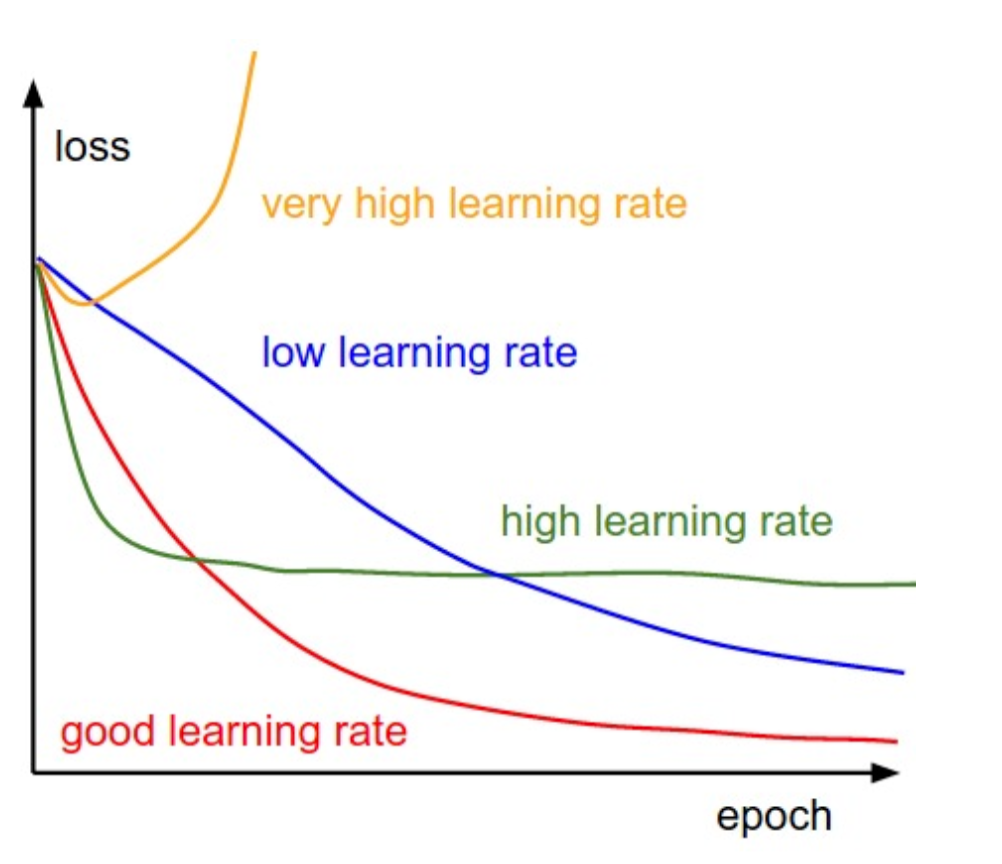
\includegraphics[width=0.5\linewidth]{img/sgd_learnrate.png}
    \caption{Graph showing a loss over epochs for different learning rates}
    \end{figure}
\end{itemize}

Convergence can be slow with mini-batch SGD, and selecting an appropriate learning rate often requires experimentation. Learning rate schedules or adaptive learning rate methods are used to adjust \( \eta \) during training to improve convergence.
\end{definitionbox}



\begin{definitionbox}{SGD with momentum (mini-batch)}


SGD with momentum is a variation of the standard SGD that accelerates convergence by incorporating a fraction of the previous weight update. Loss is defined by:

\[ \mathcal{L} = \frac{1}{n} \sum_{i} \ell(h(x_i), y_i) \]
where \( h(x_i) \) is the hypothesis function for input \( x_i \) and \( y_i \) is the true value. The gradient of the loss with respect to the weights is:
\[ \nabla_w \mathcal{L} = \frac{1}{n} \sum_{i} \nabla_w \ell(h(x_i), y_i) \]
Weights are updated by subtracting a fraction of the gradient, controlled by the learning rate \( \eta \):
\[ W_{t+1} = W_t - \eta \nabla_w \mathcal{L}(W_t) \]

It introduces the momentum term \( \beta \) which determines the contribution of past gradients to the current direction:
\[ Z_{t+1} = \beta Z_t + \nabla_w \mathcal{L}(W_t) \]

Momentum accumulates with past updates.\\


The weight update rule is then modified to:
\[ W_{t+1} = W_t - \eta Z_{t+1} \]
where \( \beta \) typically has a value around 0.9. When \( \beta = 0 \), this reduces to the standard SGD. The momentum term helps in smoothing out the updates and can lead to faster convergence.

\begin{figure}[H]
    \centering
    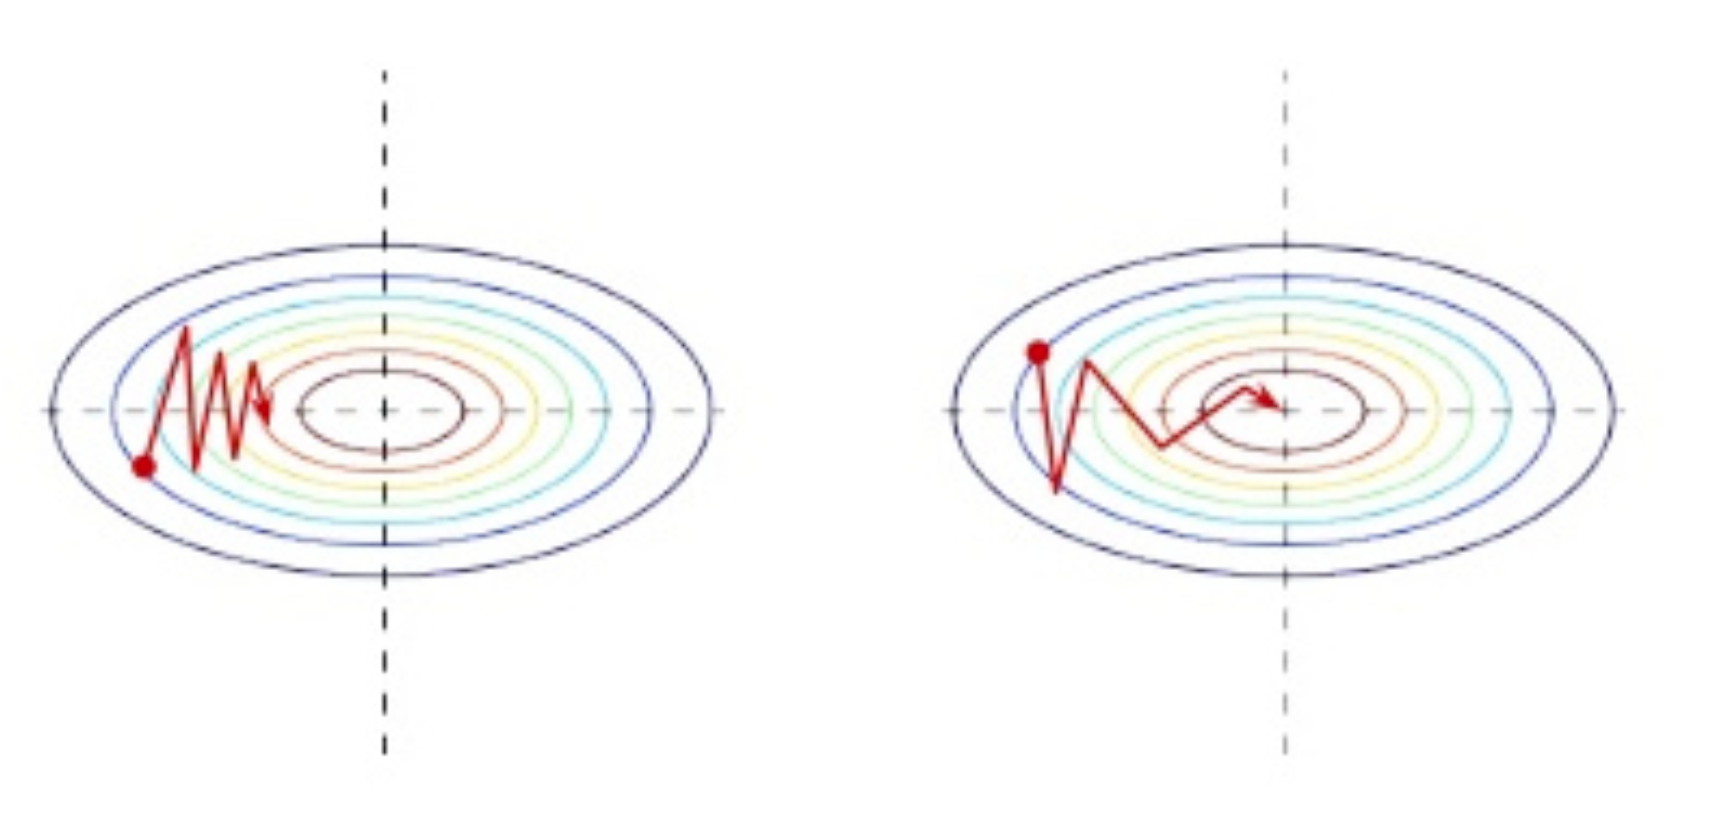
\includegraphics[width=0.5\linewidth]{img/sgd_mom.png}
    \caption{For momentum-based SGD, for any component where the gradient is heading in the intended direction, momentum is accumulated in that direction. In this example, note a horizontal acceleration towards the centre.}
    
\end{figure}
\end{definitionbox}

\begin{definitionbox}{SGD with Nesterov momentum}
Stochastic Gradient Descent (SGD) with Nesterov momentum is an optimisation technique that aims to accelerate SGD by taking into account the direction of the previous gradient step. It is described as follows:
\begin{itemize}
    \item The loss \( \mathcal{L} \) is computed as the average of the loss function \( \ell \) over all examples \( x_i \) in the mini-batch:
    \[ \mathcal{L} = \frac{1}{n} \sum_{i} \ell(h(x_i), y_i) \]
    \item The gradient of the loss with respect to the weights is:
    \[ \nabla_w \mathcal{L}(W) = \frac{1}{n} \sum_{i} \nabla_w \ell(h(x_i), y_i) \]
    \item The Nesterov momentum update is defined as:
    \[ Z_{t+1} = \beta Z_t + \nabla_w \mathcal{L}(W_t - \eta\beta Z_t) \]
    Note the lookahead step occurring in the loss function. Compare this to basic momentum given by:
    \[ Z_{t+1} = \beta Z_{t} + \nabla_w \mathcal{L}(W_t) \]
    Nesterov momentum involves calculating the decaying moving average of the gradients of projected positions in the search space rather than the actual positions themselves.


    \item The weight update formula is then:
    \[ W_{t+1} = W_t - \eta Z_{t+1} \]
\end{itemize}
Nesterov momentum improves upon standard momentum by refining the direction of the step not only with the current gradient but also by looking ahead at where the next step would take the optimisation process. This anticipatory update prevents us from going too fast and results in more responsive gradient steps.

Nesterov momentum involves:
\begin{enumerate}
    \item Making a step in the direction of the accumulated gradient.
    \item Measuring the gradient in this new point and correct the direction.
\end{enumerate}
This approach can significantly accelerate the convergence of SGD, especially in the context of high curvature, noisy gradients, or small mini-batches.
\begin{figure}[H]
    \centering
    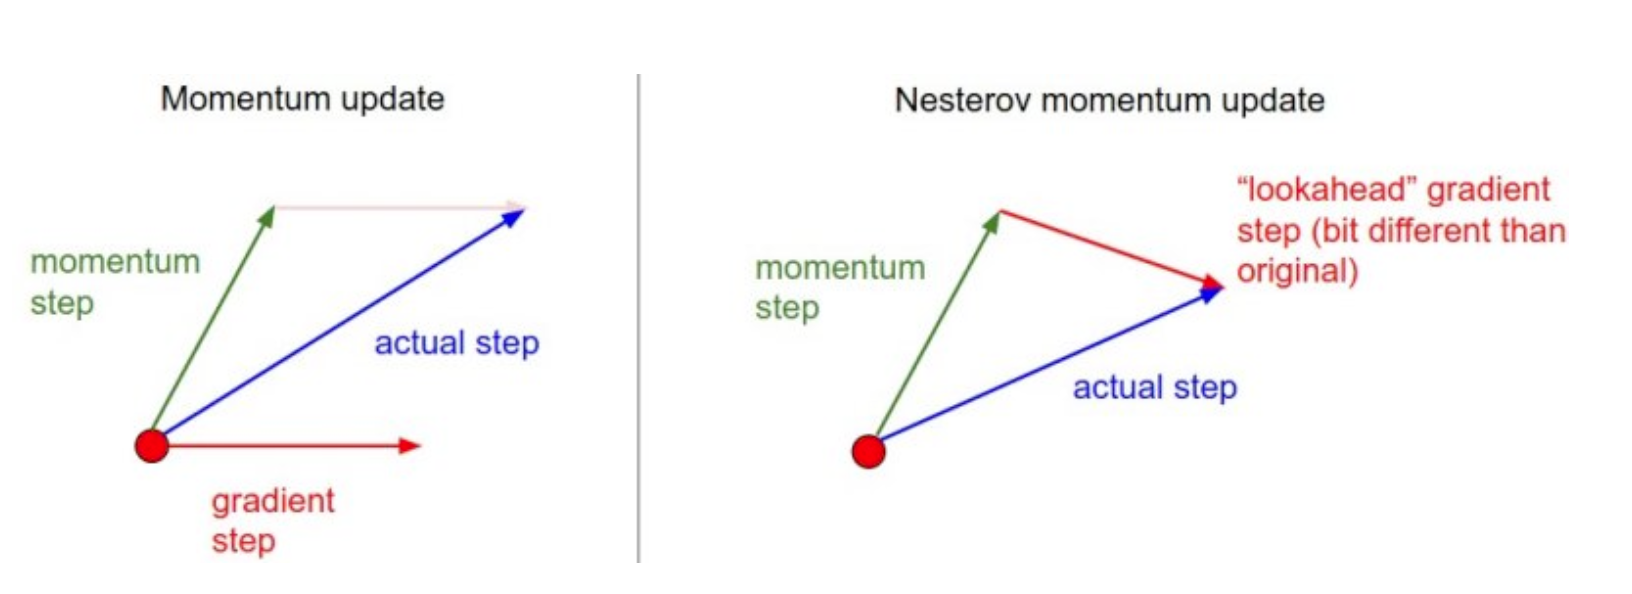
\includegraphics[width=0.7\linewidth]{img/nesterov.png}
    \caption{Lookahead gradient visualisation}
    
\end{figure}
\end{definitionbox}

\begin{definitionbox}{Adagrad}
Adagrad is an optimisation algorithm designed to adapt the learning rate to the parameters, performing smaller updates for parameters associated with frequently occurring features, and larger updates for parameters associated with infrequent features. It is particularly well-suited for dealing with sparse data. The Adagrad update rule is defined as follows:
\begin{itemize}
    \item The weight update rule is:
    \[ W_{t+1} = W_t - \frac{\eta}{\sqrt{G_t + \epsilon}} \odot \nabla_w \mathcal{L}(W_t) \]
    where \( G_t \in \mathbb{R}^{p \times p} \) is a diagonal matrix where each diagonal element \( i, i \) is the sum of the squares of the gradients with respect to \( w_i \) up to iteration \( t \), \( \eta \) is the learning rate, and \( \epsilon \) is a small smoothing term to prevent division by zero.
    \item Adagrad adapts the learning rate for each parameter, reducing the learning rate monotonically for each parameter.
    \item It has been used effectively in training GloVe word embeddings, among other applications.
    \item However, the monotonic decrease can sometimes lead to premature and excessive reduction in the effective learning rate, causing the algorithm to stop learning.
\end{itemize}

Intuitively, we are trying to step the weights vector through a (generally high) dimensional space trying to minimise the loss function. This is done by moving in the opposite direction to gradient. However, not all dimensions are equal. Some consistently receive larger gradients, some receive smaller gradients. If we use a uniform learning rate, we might step too far in directions with large gradients (potentially overshooting the minimum), and too little with small gradients (taking too long to converge). The diagonal matrix \(G\) is used to keep track of historical gradients, serving as an automatic tuning dial for learning rates.
\end{definitionbox}

\begin{definitionbox}{RMSProp}
RMSProp (Root Mean Square Propagation) is an adaptive learning rate method that adjusts the learning rate for each weight individually. It modifies the general gradient descent weight update rule as follows:
\begin{itemize}
    \item The weight update rule is:
    \[ W_{t+1} = W_t - \frac{\eta}{\sqrt{E[\nabla \mathcal{L}^2]_t + \epsilon}} \odot \nabla_w \mathcal{L}(W_t) \]
    \item The expected squared gradient \( E[\nabla \mathcal{L}^2]_t \) is the exponentially decaying average of squared gradients:
    \[ E[\nabla \mathcal{L}^2]_t = \gamma E[\nabla \mathcal{L}^2]_{t-1} + (1 - \gamma)(\nabla \mathcal{L}_t)^2 \]
\end{itemize}
Intuitively, RMSProp uses the magnitude of recent gradients to normalised the gradient; this is akin to adjusting the step size depending on the 'steepness' of the learning landscape. It prevents oscillations in directions with large gradients and allows for faster progress in directions with small gradients.
\end{definitionbox}

\begin{definitionbox}{Adadelta}
Adadelta is an extension of Adagrad that seeks to reduce its aggressive, monotonically decreasing learning rate. Instead of accumulating all past squared gradients, Adadelta limits the window of accumulated past gradients to some fixed size. The update rule is:
\begin{itemize}
    \item The weight update rule is:
    \[ W_{t+1} = W_t - \frac{\sqrt{E[\Delta W^2]_{t-1} + \epsilon}}{\sqrt{E[\nabla \mathcal{L}^2]_t + \epsilon}} \odot \nabla_w \mathcal{L}(W_t) \]
    \item The update accumulation \( E[\Delta W^2]_t \) is computed as:
    \[ E[\Delta W^2]_t = \gamma E[\Delta W^2]_{t-1} + (1 - \gamma)(W_t - W_{t-1})^2 \]
\end{itemize}
Intuitively, Adadelta adapts the learning rate based on a moving window of gradient updates, rather than accumulating all past squared gradients. This allows the learning rate to remain more robust and not decay to infinitesimally small values, which addresses the vanishing learning rate problem of Adagrad.
\end{definitionbox}

\begin{definitionbox}{Adam (Adaptive Moment Estimation)}
Adam is an optimisation algorithm that computes adaptive learning rates for each parameter by estimating the first and second moments of the gradients. Its update rule combines the advantages of two other extensions of stochastic gradient descent, AdaGrad and RMSProp. Specifically, the Adam update rule is given by:
\begin{itemize}
    \item The weight update rule is:
    \[ W_{t+1} = W_t - \frac{\eta}{\sqrt{v_t + \epsilon}} \odot m_t \]
    \item The first moment \( m_t \) and second moment \( v_t \) estimates are:
    \[ m_t = \frac{\beta_1 m_{t-1} + (1 - \beta_1) \nabla_w \mathcal{L}_t}{1 - \beta_1^t} = \frac{\mathbb{E}\left[ \nabla_w \mathcal{L}_t\right]}{1 - \beta_1^t} \]
    \[ v_t = \frac{\beta_2 v_{t-1} + (1 - \beta_2) (\nabla_w \mathcal{L}_t)^2}{1 - \beta_2^t} = \frac{\mathbb{E}\left[ \nabla_w \mathcal{L}_t\right]}{1 - \beta_1^t} \]
\end{itemize}
Intuitively, Adam performs smaller updates for parameters associated with frequently occurring features and larger updates for parameters associated with infrequent features. It uses the squared gradients to scale the learning rate and takes advantage of momentum by using the moving average of the gradient. It corrects for the initial bias towards zero in the first and second moment estimates, providing a more accurate update step.

Commonly used values for the decay parameters are \( \beta_1 \approx 0.9 \), \( \beta_2 \approx 0.999 \), and \( \epsilon \approx 10^{-8} \), which control the exponential decay rates for these moment estimates.
\end{definitionbox}

\subsection{Comparison of Optimisers}
\begin{figure}[H]
    \centering
    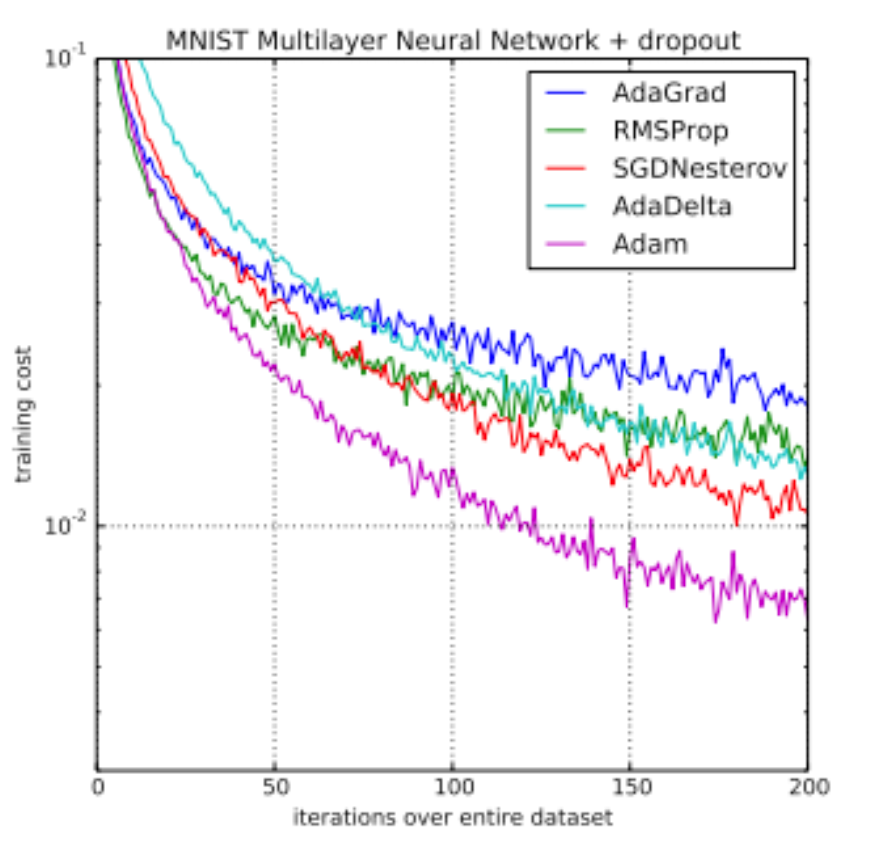
\includegraphics[width=0.5\linewidth]{img/optimisers.png}
    \caption{Comparison of training cost over iterations for different optimisers]}
    
\end{figure}

\begin{itemize}
    \item Adagrad introducing an adaptive learning rate, best suited for sparse data.
    \item RMSProp resolves vanishing learning rates by using decaying averages
    \item Adadelta is similar to RMSProp but does not require a learning rate
    \item Adam is RMSProp + Momentum, also adds bias correction
    \item SGD is often used, tends to find a good minimiser and generalises well
\end{itemize}

\section{Regularisation}
\subsection{Dropout}
\subsection{Distribution Problem}
\subsection{Batch Normalisation}
\section{Network Design}
\subsection{Baseline}
\subsection{Finetuning}
\subsection{Data Collection}
\subsection{Validation}
\subsection{Data Augmentation}
\subsection{Adversarial Training}
\subsection{Setting Parameters}
\subsection{Monitoring and Debugging}





\chapter{CNN Architectures}

\section{Introduction}

This portion of the course provides a high-level overview on the history and evolution of convolutional neural networks, providing information on each advancement. This document will cover very brief summaries, it is advised to consult the slides for more reading.


\section{The CNN data}
\textbf{ImageNet Large Scale Visual Recognition Challenge (ILSVRC)}
\begin{itemize}
    \item The standard benchmark for comparing recognition systems (CNNs in this case)
    \item An annual competition since 2010, with 1.2 million images across 1000 classes
\end{itemize}

\section{CNN models}
\subsubsection{1989-1998  LeNet by Yann LeCun et all.}
\begin{itemize}
    \item 2 conv layers, 2 pooling layers, 2 FC layers, 60k parameters
    \item  \texttt{INPUT $\rightarrow$ CONV $\rightarrow$ SIGMOID $\rightarrow$ POOL $\rightarrow$ CONV $\rightarrow$ SIGMOID $\rightarrow$ POOL $\rightarrow$ FC $\rightarrow$ SIGMOID $\rightarrow$ FC}

    \item 99\% accuracy on MNIST
\end{itemize}

\subsubsection{2012 AlexNet by Alex Krizhevsky et al.}
\begin{itemize}
    \item Used LeNet with more data and GPUs.
    \item Increased from 2 to 5 conv layers, + 1 FC layer(now 3 layers) , each followed by ReLU instead of tanh, the activation function is 6 times faster
    \item Dropout 0.5 for FC layers instead of L2 regularisation. Training time doubled as a result
    \item 2 pooling layers to reduce netwok size
    \item 62.3M parameters, with conv layers representing 6\% of all parameters and 95\% of the total computation
    \item Top-5 error rate of 15.3\% on ImageNet at time of release
\end{itemize}

\subsubsection{2014 VGG by Karen Simonyan et al.}
\begin{itemize}
    \item Based on AlexNet, but replaced large filters in first two layers with $3\times 3$ filters.
    \item Use multiple stacked smaller size kernels
    \item Increase the representational capacity of the ConvNet for the same number of parameters
    \item Double the channels, use ReLU to avoid saturation
    \item Same number of FC layers.
    \item 138M parameters
    \item Top-5 error rate of 7.3\% on ImageNet at time of release
    \item Note: at this rate, networks are getting deeper and deeper due to gaining more filters. There is a risk of saturation and degraded performance
\end{itemize}

\subsubsection{2014 GoogLeNet by Christian Szegedy et al.}
\begin{itemize}
    \item Utilised the inception block – filters with multiple sizes that operate on the same level to capture different scales of detail. Goes for a wider approach instead of a deep approach
    \item Auxiliary classifiers used during training: they are like a``mini cnn" with conv layers, activation functions, pooling layers, and fc layers, that provide intermediate outputs. They make predictions based on features available and are a form of providing intermediate layers, they help reduce the vanishing gradient problem, by providing additional gradients.
    \item Max pooling followed by $1\times 1$ convolution to reduce depth before the $ 3 \times 3$ and $5 \times 5$ convolutions
    \item Uses global average pooling instead of FC layers
    \item Version 2 uses factorised filters to help improve speed.
    \item Top-5 error rate of 6.67\% on ImageNet at time of release (V1)
    \item V4 achieved lowest of 5\%
\end{itemize}

\subsubsection{2015-2016 Residual NN (ResNet) by Kaiming He et al.}
\begin{itemize}
    \item Utilised identity mappings in layers to allow for stacking layers without reducing network performance.
    \begin{figure}[H]
        \centering
        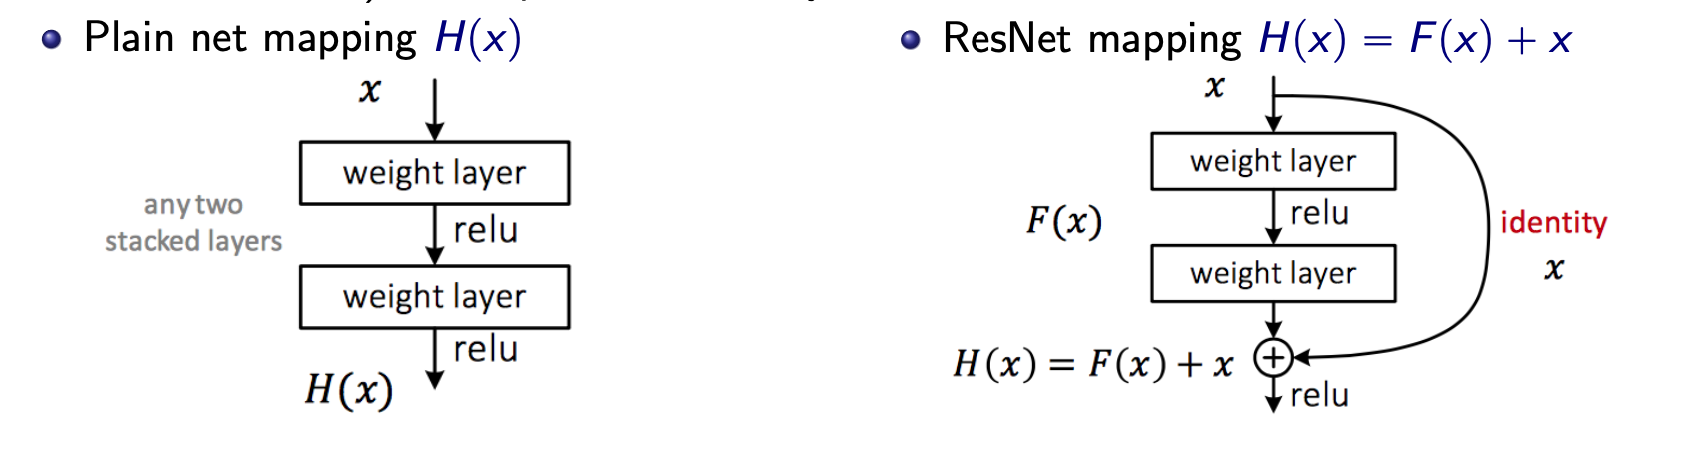
\includegraphics[width=0.7\linewidth]{img/resnet.png}
        
        
    \end{figure}
    \item The identity mapping allows the gradient to skip 1 or more layers using an ``identity shortcut connection"
    \item Skip connections allow the network to learn an identity function, which ensures that the higher layer will perform at least as well as the lower layer, and not worse.

    \item The identity skip connections enable the stacked layers to learn a residual mapping, which is essentially the difference between the desired underlying mapping and the identity function.
    
    \item The hypothesis is that it is easier to let the stacked layers learn (fit) this residual mapping than to learn the desired underlying mapping directly. 


    \item 2016 paper proposed 18, 50, 101, 152, 200 layer variants
    \item Most filters are $3 \times 3$ with global average pooling followed by the classification layer
    \item ResNet-200 achieved Top-5 error rate of 4.8\% on ImageNet at time of release, beating human performance
\end{itemize}

\subsubsection{2017 ResNeXt by Microsoft Research}
\begin{itemize}
    \item Combination of Google's Inception module and Kaiming He's skip connections
    \item Achieved Top-5 error rate of 4.4\% on ImageNet at time of release
\end{itemize}

\subsubsection{2017 DenseNet by Huang Gao et al.}
\begin{itemize}
    \item Allows skipping across multiple layers.
    \item ResNet: \( x_l = F_l(x_{l-1}) + x_{l-1} \)
    \item DenseNet: \( x_l = F_l([x_0, x_1, \ldots, x_{l-1}]) \)
    \item Achieves a stornger gradient flow, parameter and computational efficiency, and maintains low complexity features

\begin{figure}[H]
    \centering
    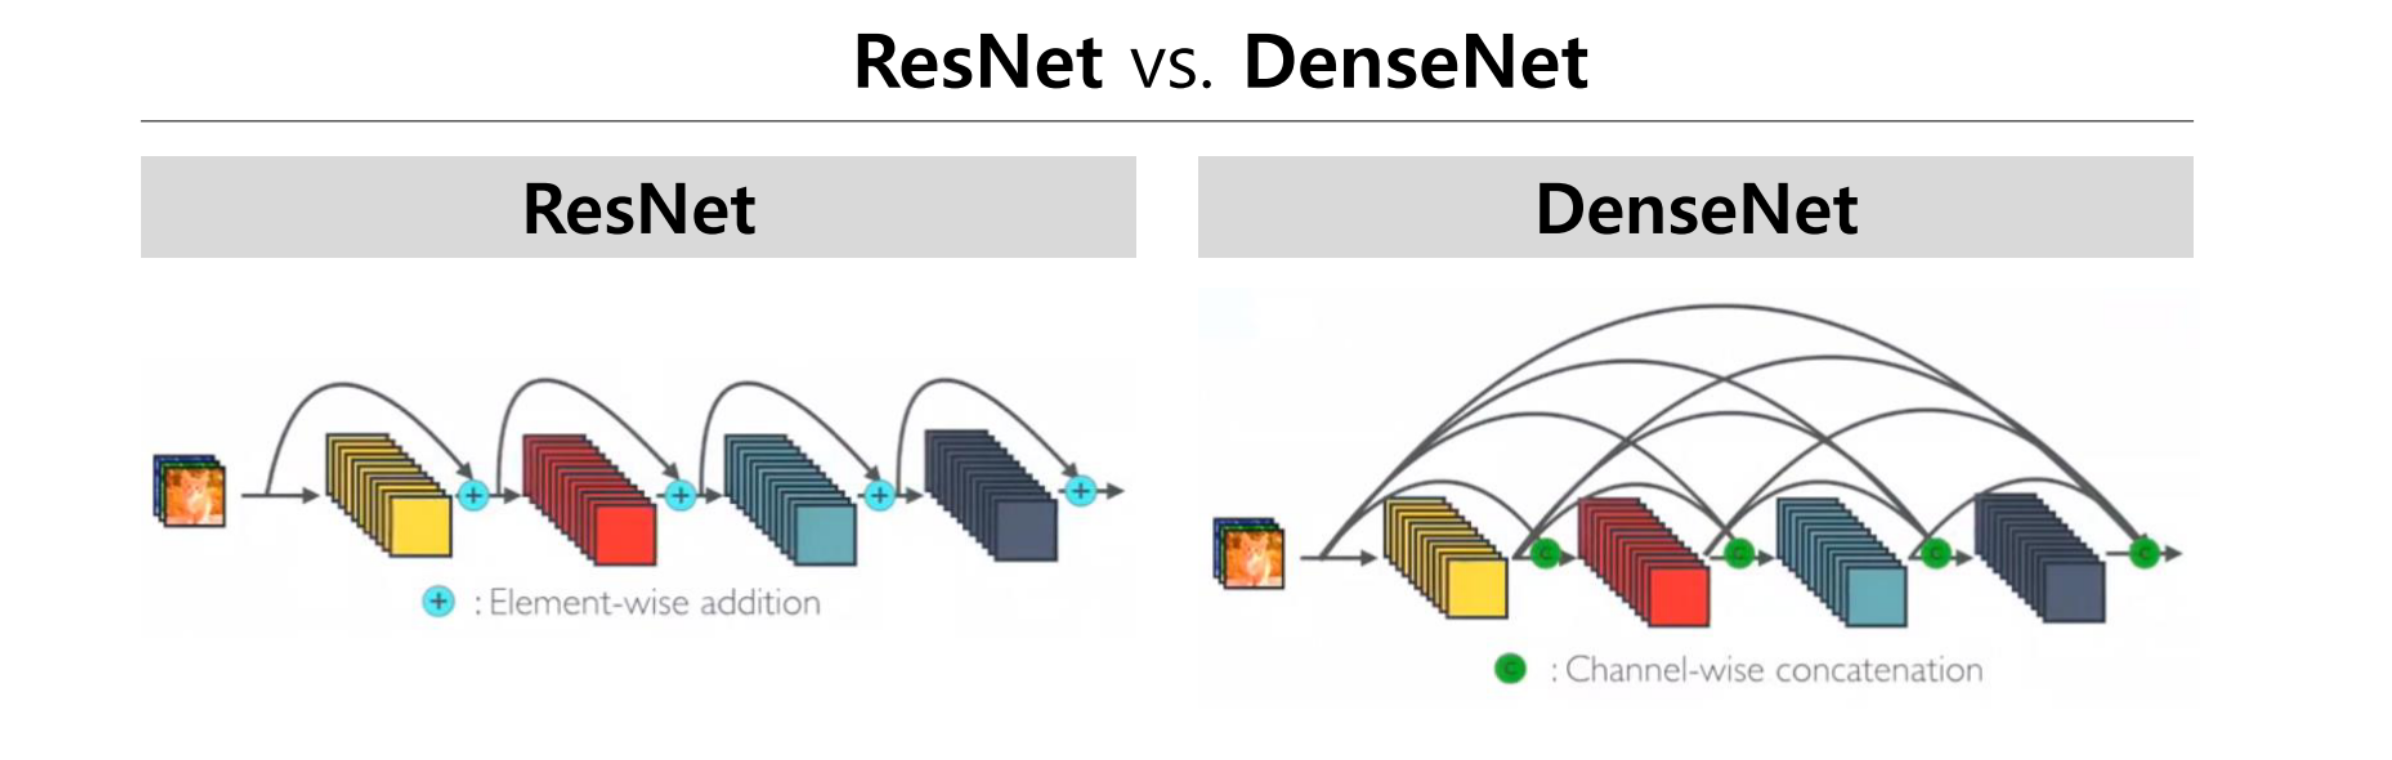
\includegraphics[width=0.75\linewidth]{img/densenet_resnet.png}
    
    
\end{figure}

\end{itemize}

\subsection{Performance Comparison}
\begin{figure}[H]
    \centering
    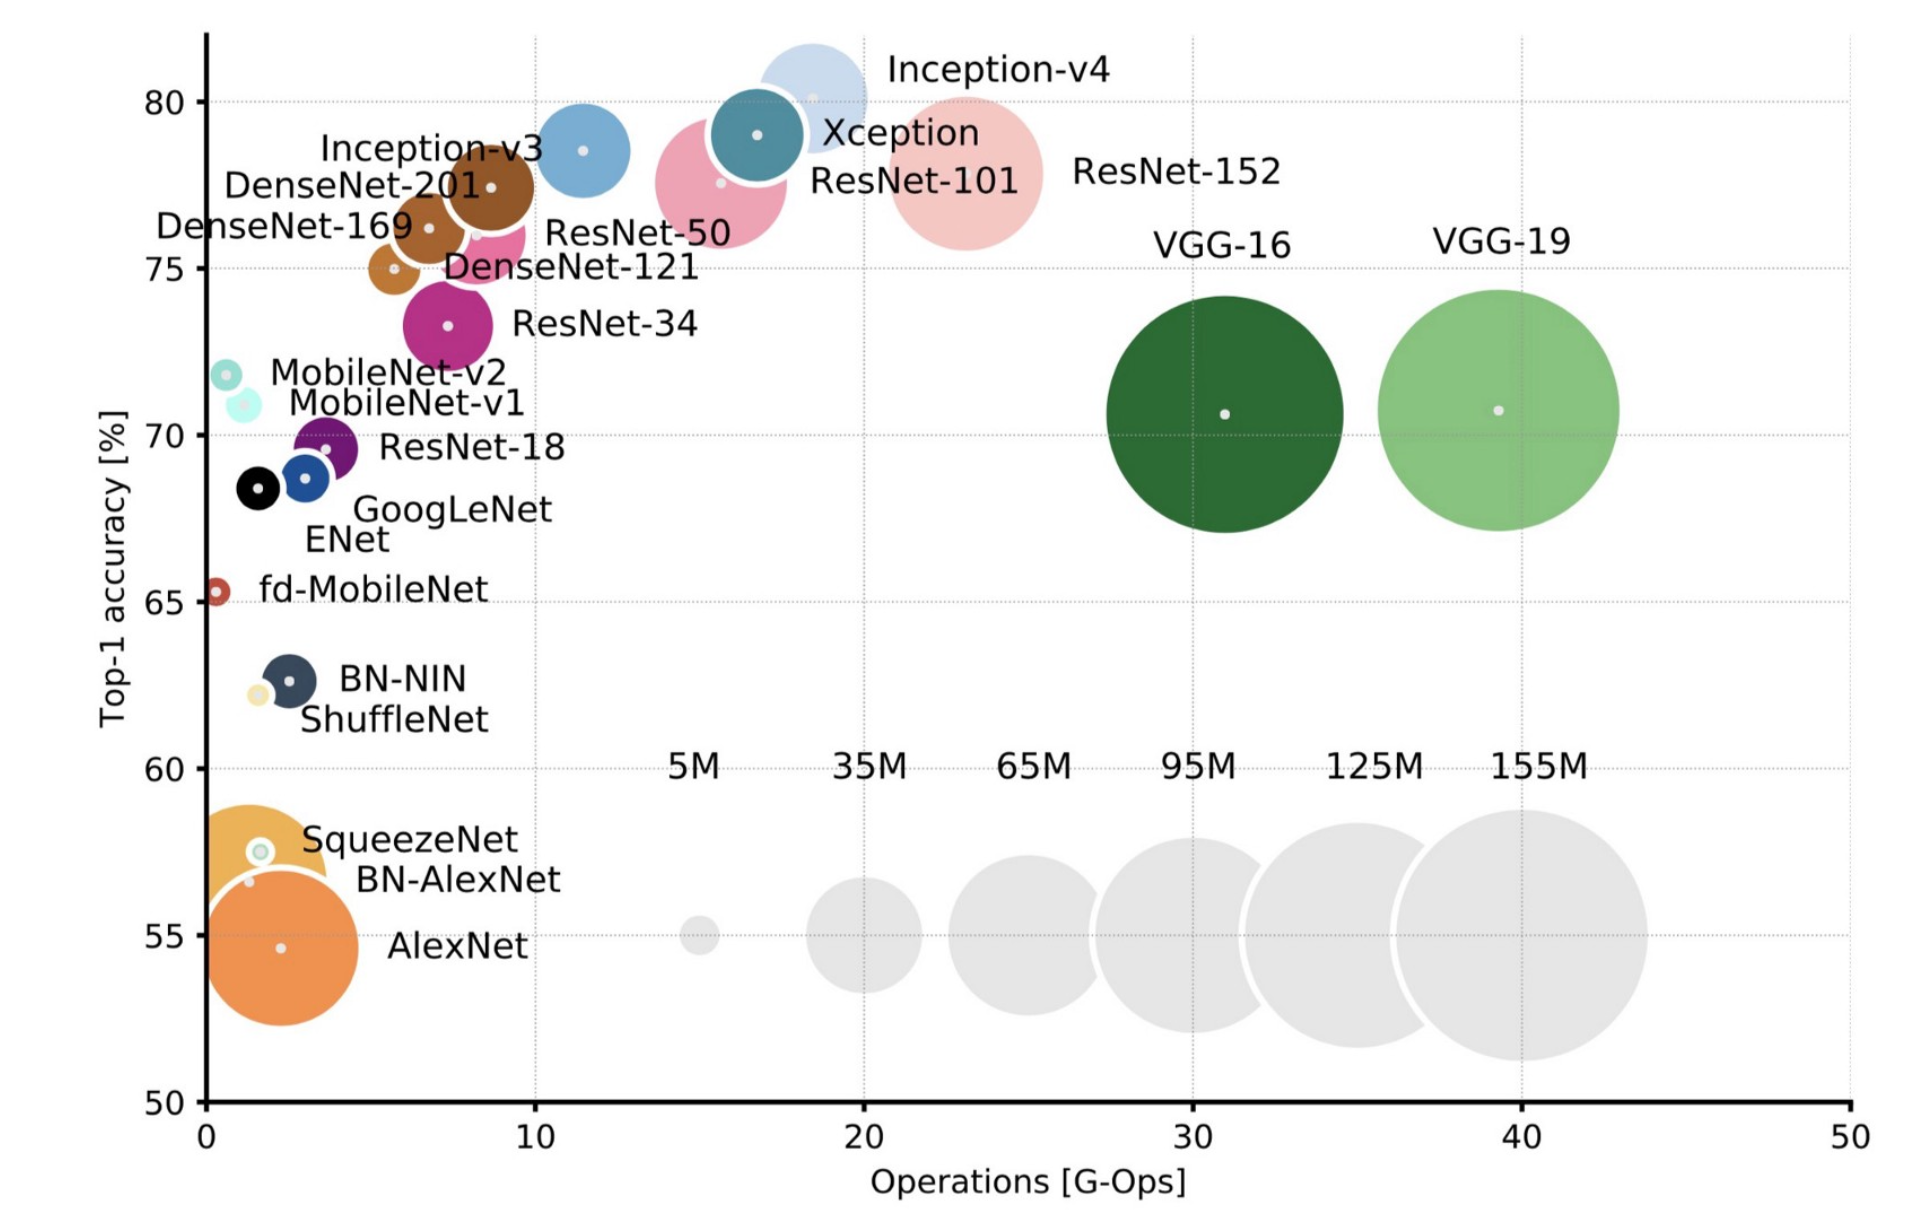
\includegraphics[width=0.8\linewidth]{img/cnn_performance.png}
    
    
\end{figure}

\subsection{CNN Encoder-Decoder Architecture}
\begin{itemize}
    \item Used for dense prediction tasks e.g. image segmentation, image enhancement, etc. Takes in an image and outputs and image.
    \item Typically, the encoder extracts feature maps by compressing input data into a condensed representation known as feature maps.
    \item The decoder's role is typically to take encoded feature maps and upsample/reconstruct them back to a desired input resolution (usually the original resolution), recovering spatial details that might have been compressed during encoding.
\end{itemize}

\subsubsection{Fully Convolutional Networks (FCN) by Long et al. (2015)}
\begin{itemize}
    \item Build FCNs that take input or arbitrary size and produce similarly sized output with efficient inference and learning
    \item Fully connected layers are viewed as convolutions with kernels that cover their entire input regions
    \item Upsampling done with backwards strided convolution

    \begin{figure}[H]
        \centering
        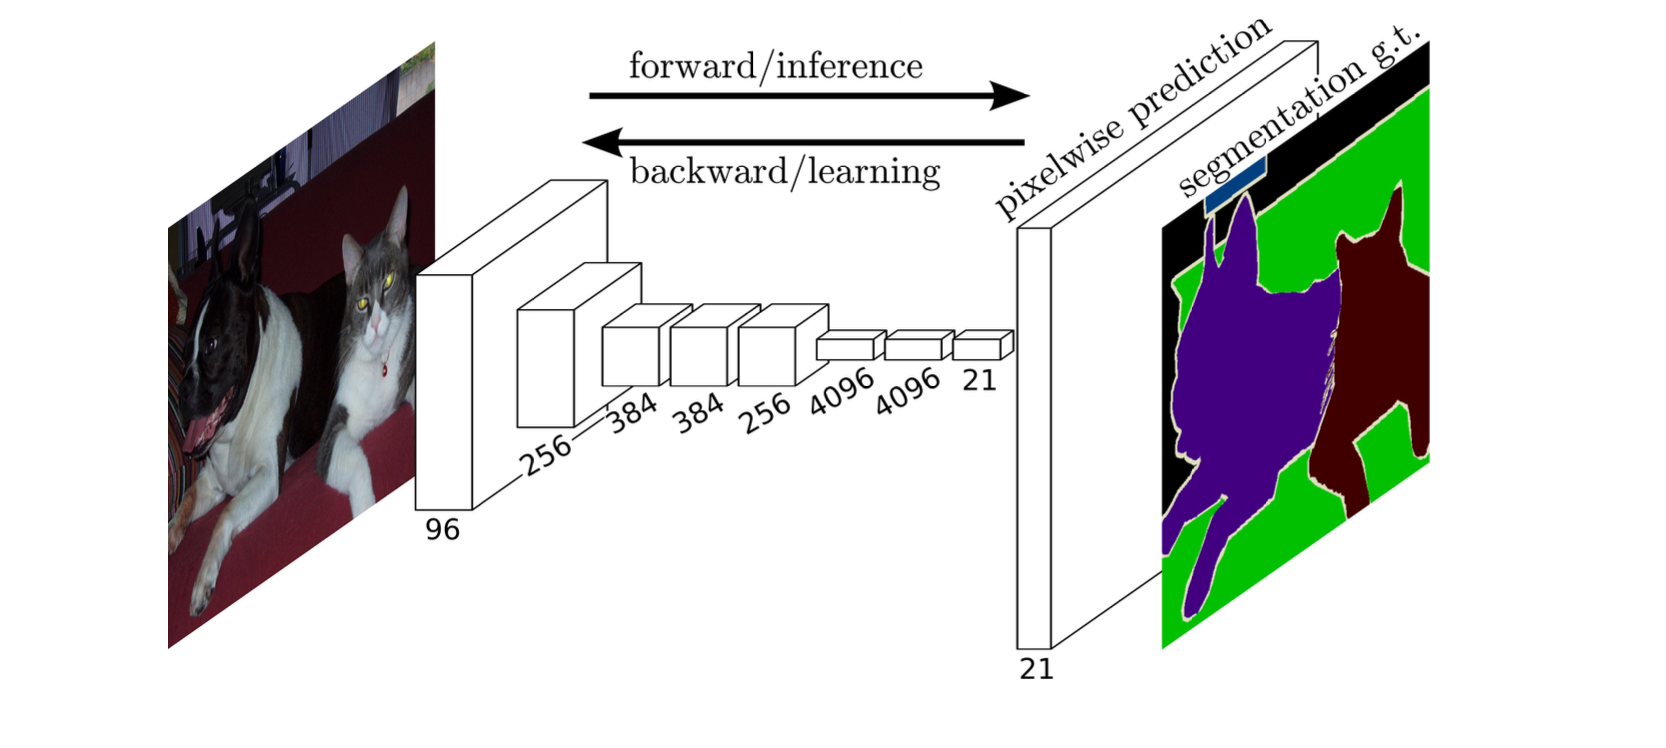
\includegraphics[width=0.75\linewidth]{img/FCN.png}
        
        
    \end{figure}
    
\end{itemize}

\subsubsection{U-Net by Ronneberger et al. (2015}
\begin{itemize}
    \item U-shaped architecture with skip connections and multi-scale feature maps
    \item Slightly more symmetrical than the FCN
    \begin{figure}[H]
        \centering
        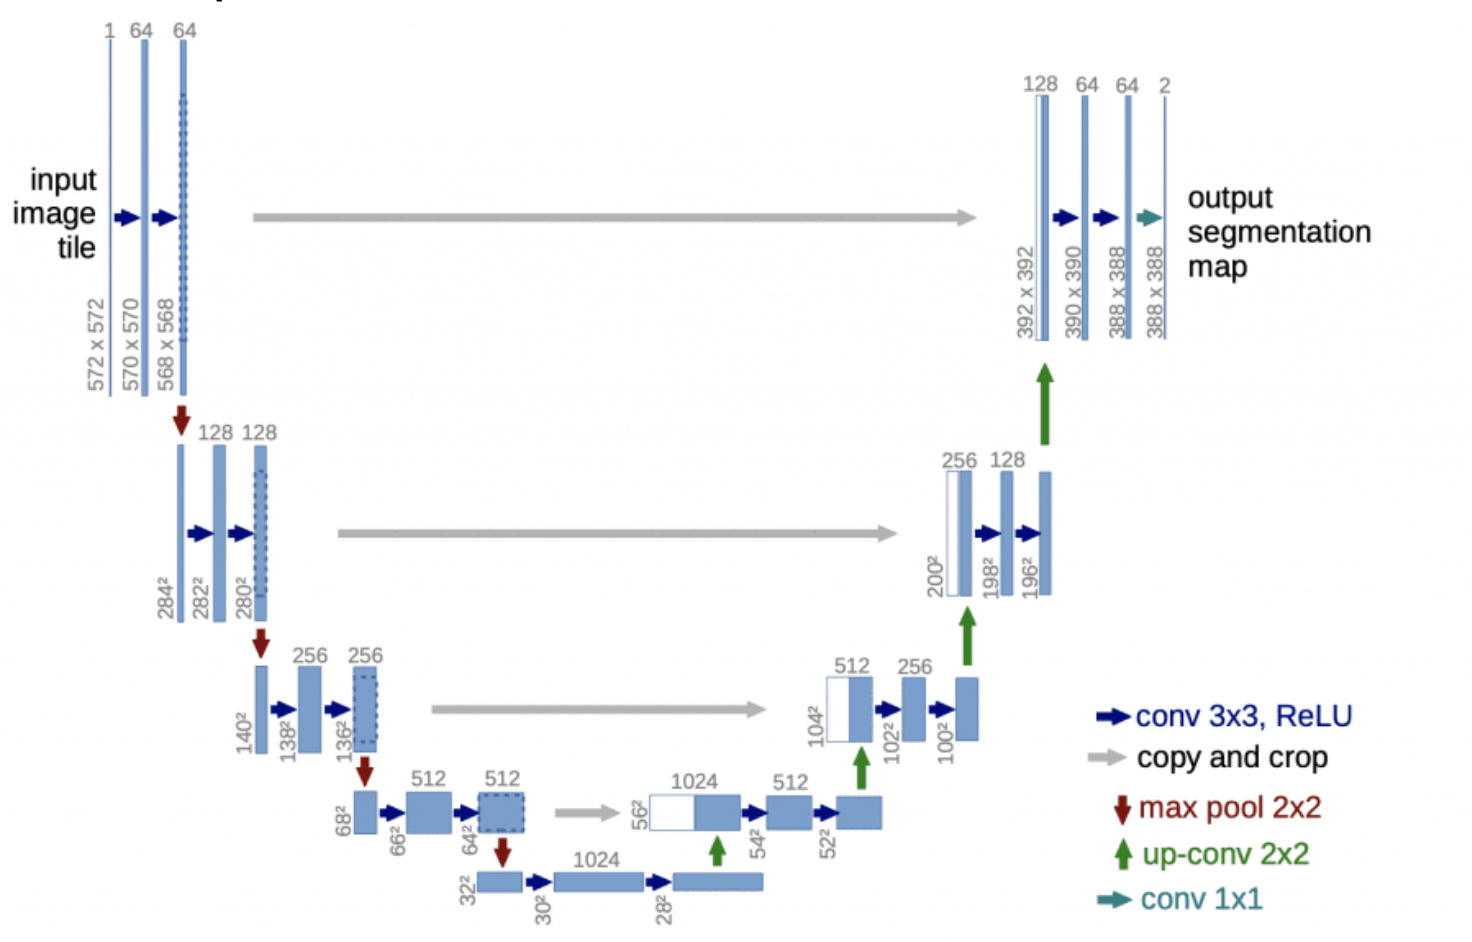
\includegraphics[width=0.5\linewidth]{img/u_net.png}
        
        
    \end{figure}
\end{itemize}

\subsubsection{CNN Siamese Networks}
\begin{itemize}
    \item Two networks in parallel trying to discern the transformation of an image given a before-after example
    \item L2 loss compares output features
    \item Shared FC layers possibly merge the output of two streams
    \begin{figure}[H]
        \centering
        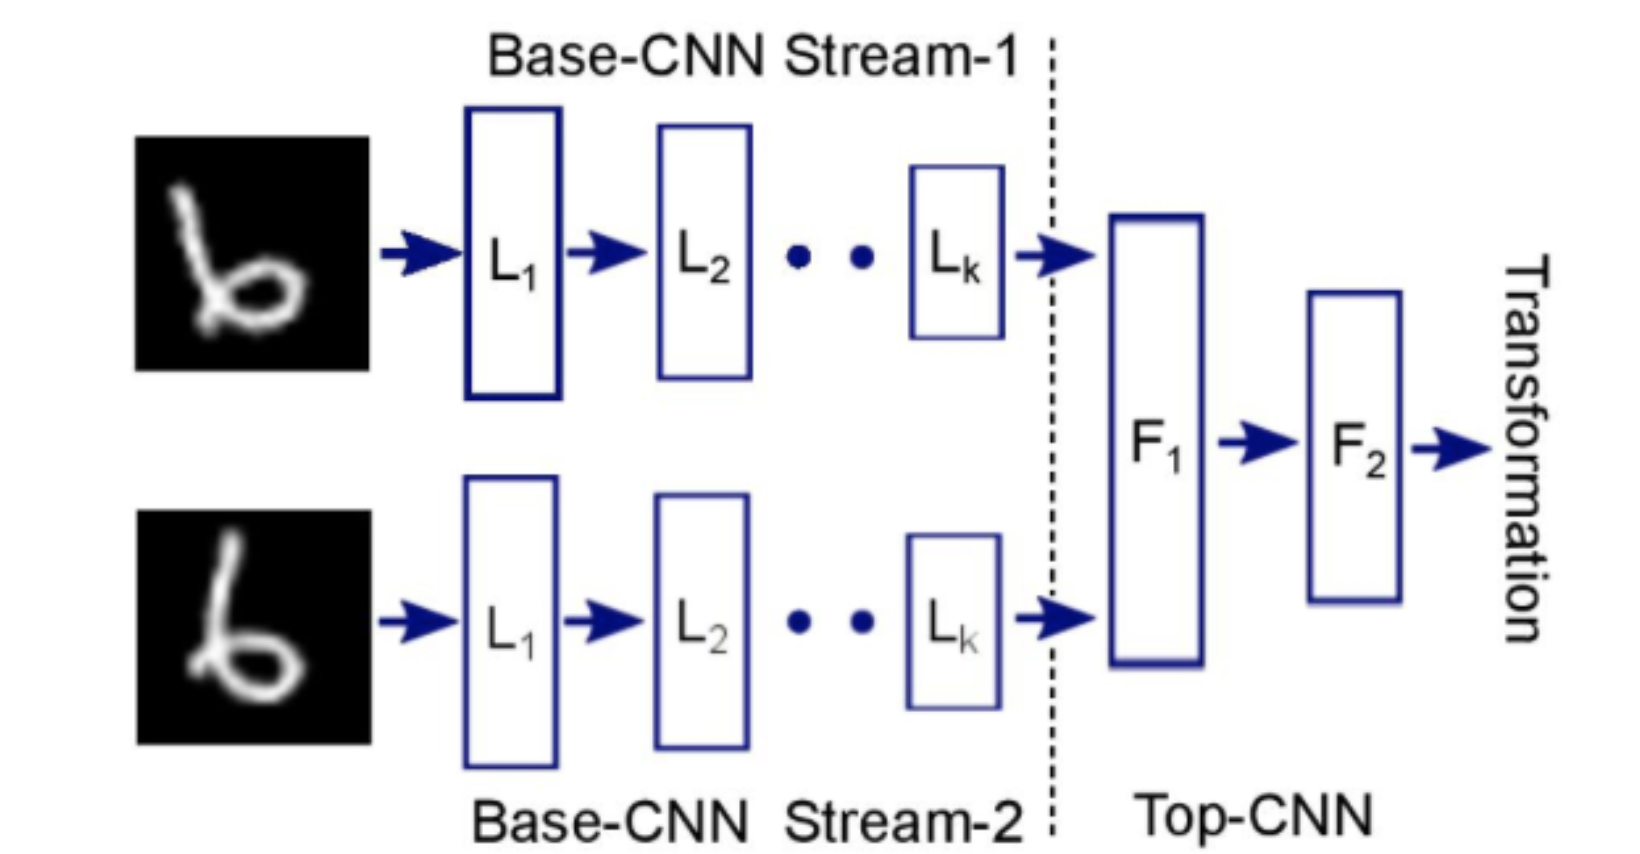
\includegraphics[width=0.75\linewidth]{img/siamese.png}
        
        
    \end{figure}
\end{itemize}

\subsubsection{Multitask Learning}
\begin{itemize}
\item Multi-task CNNs handle multiple learning tasks concurrently
\item An example could be classifying a type of animal, but also trying to localise it, determining its location with a bounding box.
\item They utilise shared layers to capture features common to all tasks, which can lead to better performance than learning separate models.
\item Task-specific layers are used on top of the shared layers to learn features unique to each task.
\item These networks can be more parameter-efficient and require less computational resources than separate models for each task. They often result in improved learning of features due to the regularising effect of jointly learning related tasks.
\end{itemize}

\begin{figure}
    \centering
    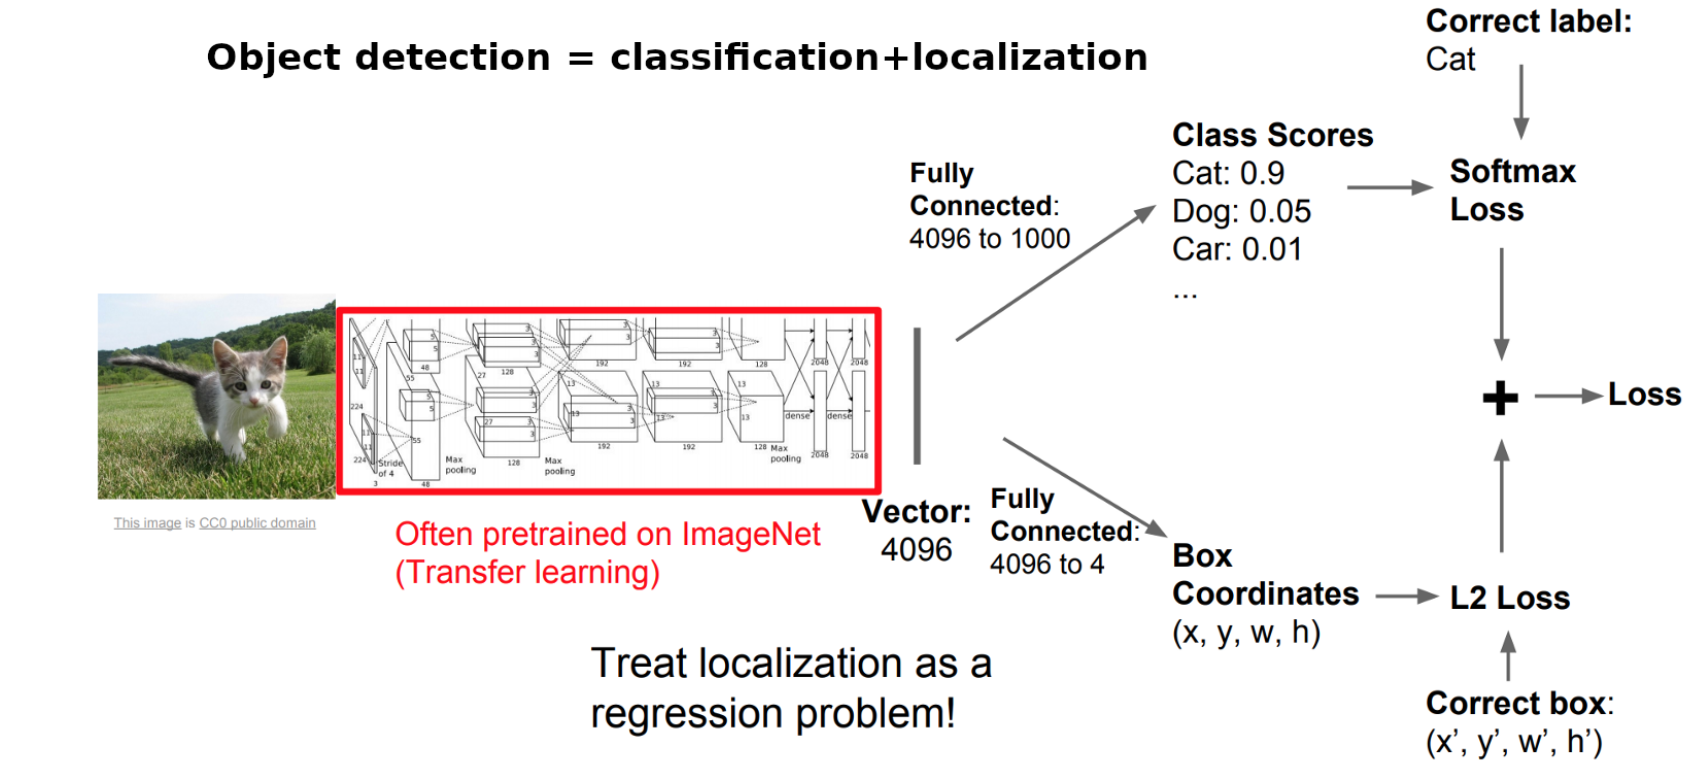
\includegraphics[width=0.75\linewidth]{img/multitask.png}
    
    
\end{figure}
\chapter{Recurrent Neural Networks}
\section{Feed-Forward Neural Networks vs Recurrent Neural Networks}

\begin{itemize}
    \item Feed-Forward Neural Networks (FFNNs) are the simplest type of artificial neural network architecture. In a FFNN, information moves in only one direction—forward—from the input nodes, through the hidden nodes (if any), and finally to the output nodes. There are no cycles or loops in the network.
    
    \item Recurrent Neural Networks (RNNs), on the other hand, have connections that form directed cycles. This means that information can be recycled in the network, allowing them to maintain a `memory' of previous inputs. This is particularly useful for tasks that require the network to remember across time steps, like language modelling and time series prediction.
    
    \item The main architectural difference is that RNNs have a recurrent hidden state whose activation at each time is dependent on that of the previous time step, which is not the case for FFNNs.
\end{itemize}
\begin{figure}[H]
    \centering
    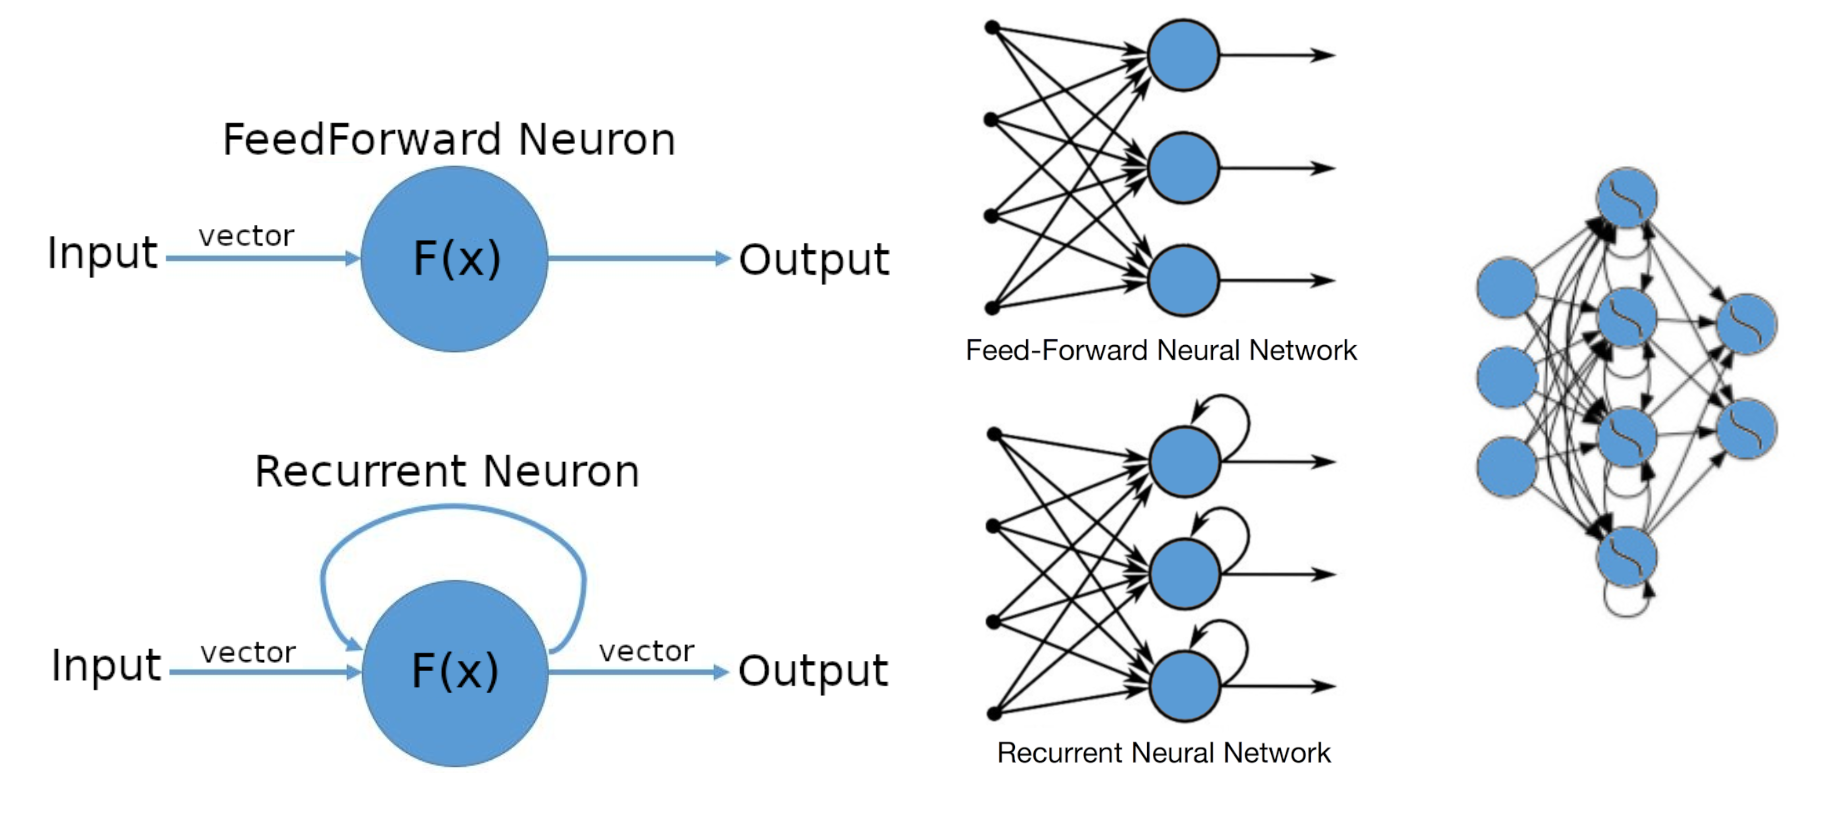
\includegraphics[width=0.75\linewidth]{img/ffnn_vs_rnn.png}
\end{figure}

\section{Structure of RNNs}
\begin{itemize}
    \item Recurrent Neural Networks (RNNs) exhibit a chain-like structure, making them particularly suitable for processing sequences and lists such as speech, language, text, and temporal data like audio and video streams.
    \item The architecture of RNNs allows for the handling of input and output sequences of variable lengths, a feature that is leveraged in applications such as dialog generation.
    \item In dialog generation, for instance, RNNs can be used to generate a response based on an input question. The process involves encoding the semantic meaning of words into numerical embeddings which the network uses to understand context and generate appropriate answers.
    \item The use of softmax functions at each output stage in sequence models like RNNs helps in generating suggestions or predictions for the next word in a sequence, enabling applications such as text auto-completion and machine translation.
\end{itemize}
\begin{figure}[H]
    \centering
    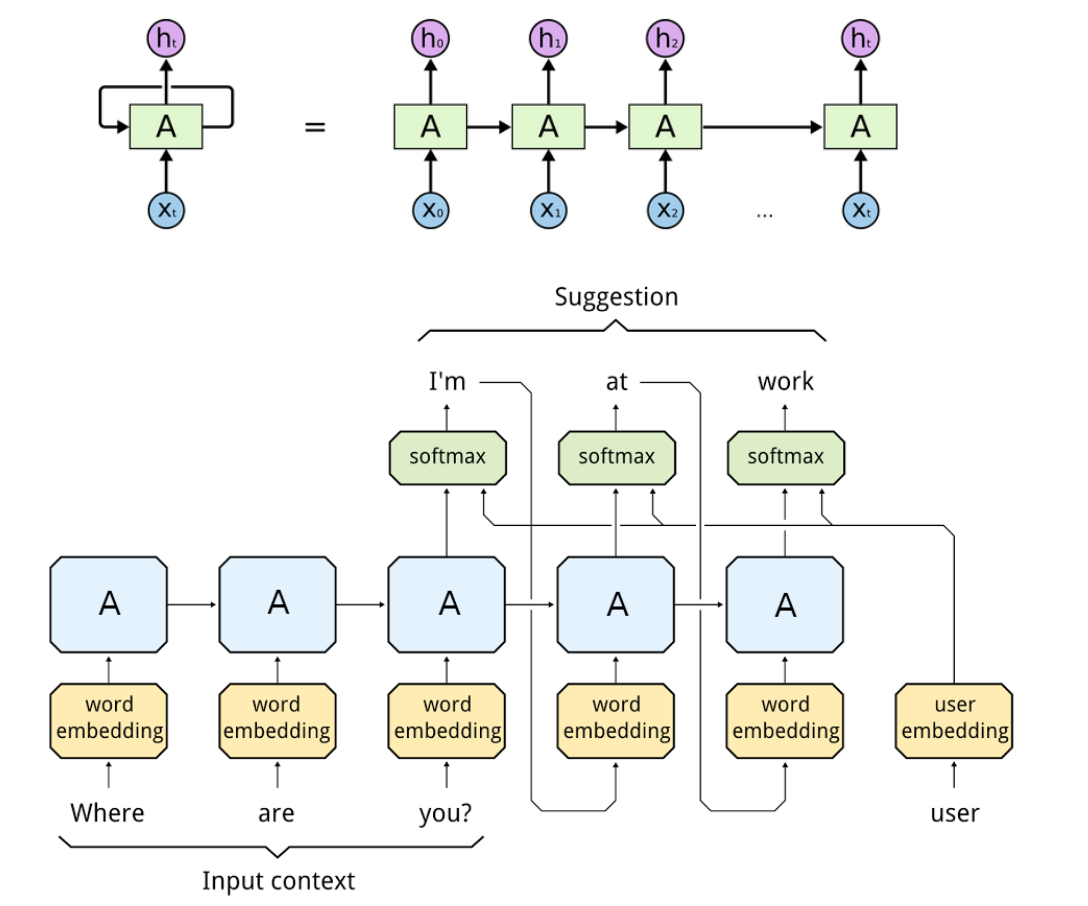
\includegraphics[width=0.5\linewidth]{img/rnn_structure.png}
    
\end{figure}


\subsection{Word Embeddings}
\begin{itemize}
    \item Word embedding is a real number-vector numerical representation of a word or text.
    \item Words with similar meanings will be closer together in the embedding space of vectors. This is to capture a sort of relationship within that space, e.g. meaning, morphology, context, etc.
\end{itemize}
\begin{figure}[H]
    \begin{center}
    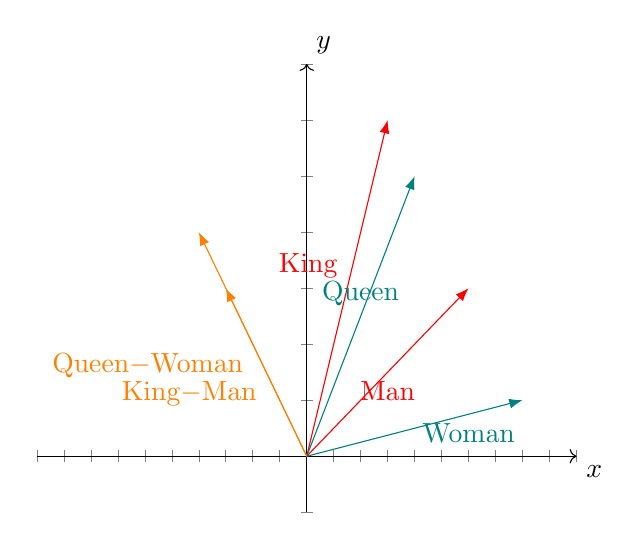
\begin{tikzpicture}
        \begin{axis}[
            xmin=-10, xmax=10,
            ymin=-1, ymax=7,
            axis lines=middle,
            axis line style={->},
            xlabel={$x$},
            ylabel={$y$},
            xtick={-10,-9,...,10},
            ytick={-1,0,...,7},
            xticklabels={,,},
            yticklabels={,,},
            xlabel style={at={(ticklabel* cs:1)},anchor=north west},
            ylabel style={at={(ticklabel* cs:1)},anchor=south west}
        ]
    
        % Vector arrows
        \draw[-{Latex},red] (axis cs:0,0) -- (axis cs:3,6) node[midway, above left] {King};
        \draw[-{Latex},teal] (axis cs:0,0) -- (axis cs:4,5) node[midway, above] {Queen};
        \draw[-{Latex},red] (axis cs:0,0) -- (axis cs:6,3) node[midway, below] {Man};
        \draw[-{Latex},teal] (axis cs:0,0) -- (axis cs:8,1) node[near end, below] {Woman};
    
        % King - Man vector
        \draw[-{Latex}, orange] (axis cs:0,0) -- (axis cs:-3,3) node[midway, below left] {King$-$Man};
    
        % Queen - Woman vector
        \draw[-{Latex}, orange] (axis cs:0,0) -- (axis cs:-4,4) node[midway, below left] {Queen$-$Woman};
        \end{axis}
    \end{tikzpicture}
    \end{center}
    \end{figure}
\begin{itemize}
    \item \textbf{One-Hot Encoding (Count Vectoring)} involves creating a binary vector for each word in the vocabulary with a 1 indicating the presence of the word in a given document and 0 indicating its absence. 
    \begin{itemize}
        \item \textbf{Example:} Given the vocabulary \{Rome, Paris, Italy, France\}, the sentence "Rome and Italy" would be vectorised as [1, 0, 1, 0]. Different lengths of sentences will still have the same length vector.
        \item \textbf{Example:} Given the vocabulary \{Rome, Paris, Italy, France\}, the sentence "I like Rome, not just Rome but Italy" would be vectorised as [1, 0, 1, 0]. 
        \item Note that it captures the words, but ignores the semantic relationship, nor its similarity or contextual meaning.
    \end{itemize}

    \item \textbf{Bag of Words} is a representation of text that describes the presence of words within a document but . It's often used in conjunction with methods like TF-IDF. It is similar to One-Hot encoding, but also keeps track of the number of occurences. 
    \begin{itemize}
        \item \textbf{Example:} Given the vocabulary \{Rome, Paris, Italy, France\}, the sentence "I like Rome, not just Rome but Italy" would be vectorised as [2, 0, 1, 0].  
        \item It does not consider the order of words.
        \item \textbf{Example:} The sentences ``Rome is a city" and``Is Rome a city?" would have the same Bag of Words representation if order is not considered.
    \end{itemize}

    \item \textbf{TF-IDF (Term Frequency-Inverse Document Frequency)} vectors weigh the frequency of a word in a document against its frequency across all documents, diminishing the importance of words that occur very frequently across documents (such as `the', `is', `and').
    \begin{itemize}
        \item \textbf{Example:} If the word ``Rome" appears often in one document but rarely in others, it will have a high TF-IDF score in that particular document.
        \item \textbf{Example: } Consider the corpus: \\
        ``I love this movie”,
        ``This movie is terrible”,
        ``The plot is confusing”\\
        \[
\begin{array}{c|cccccccc}
& \text{confusing} & \text{is} & \text{love} & \text{movie} & \text{plot} & \text{terrible} & \text{the} & \text{this} \\
\hline
\text{Document 1} & 0 & 0 & 0.51 & 0.77 & 0 & 0 & 0 & 0.39 \\
\text{Document 2} & 0 & 0.46 & 0 & 0.46 & 0 & 0.60 & 0 & 0.46 \\
\text{Document 3} & 0.53 & 0.40 & 0 & 0 & 0.53 & 0 & 0.53 & 0 \\
\end{array}
\]
        

        
    \end{itemize}

    \item \textbf{Co-occurrence Matrix} represents how often words appear together in a context within a given corpus. The matrix has a size of $V \times V$, where $V$ is the vocabulary size, and the entry at row $i$, column $j$ indicates how often the $i$-th word occurs with the $j$-th word.
    
    \begin{itemize}
        \item \textbf{Example:} In a simple corpus, the word "deep" might often occur with "learning" and less frequently with "flying", resulting in higher counts in the corresponding entries of the matrix.\\
         \[
        \begin{array}{c|cccccccc}
         & \text{I} & \text{like} & \text{enjoy} & \text{deep} & \text{learning} & \text{NLP} & \text{flying} & \text{.} \\
        \hline
        \text{I} & 0 & 2 & 1 & 0 & 0 & 0 & 0 & 0 \\
        \text{like} & 2 & 0 & 0 & 1 & 0 & 1 & 0 & 0 \\
        \text{enjoy} & 1 & 0 & 0 & 0 & 0 & 0 & 1 & 0 \\
        \text{deep} & 0 & 1 & 0 & 0 & 1 & 0 & 0 & 0 \\
        \text{learning} & 0 & 0 & 0 & 1 & 0 & 0 & 0 & 1 \\
        \text{NLP} & 0 & 1 & 0 & 0 & 0 & 0 & 0 & 1 \\
        \text{flying} & 0 & 0 & 1 & 0 & 0 & 0 & 0 & 1 \\
        \text{.} & 0 & 0 & 0 & 0 & 1 & 1 & 1 & 0 \\
\end{array}
        \]
    \end{itemize}

    \item \textbf{Word2Vec and Doc2Vec}
        \begin{itemize}
        \item Both forms utilise a shallow neural network architecture trained on large corpora to detect word usage patterns.
        \item The model effectively captures semantic relationships between words, allowing for operations like vector addition and subtraction to reveal analogous relationships.
        \item Word2Vec accounts for single-word contexts whereas Doc2Vec extends to multi-word document contexts, encapsulating more complex structures.
    \end{itemize}
    \begin{figure}[H]
        \centering
        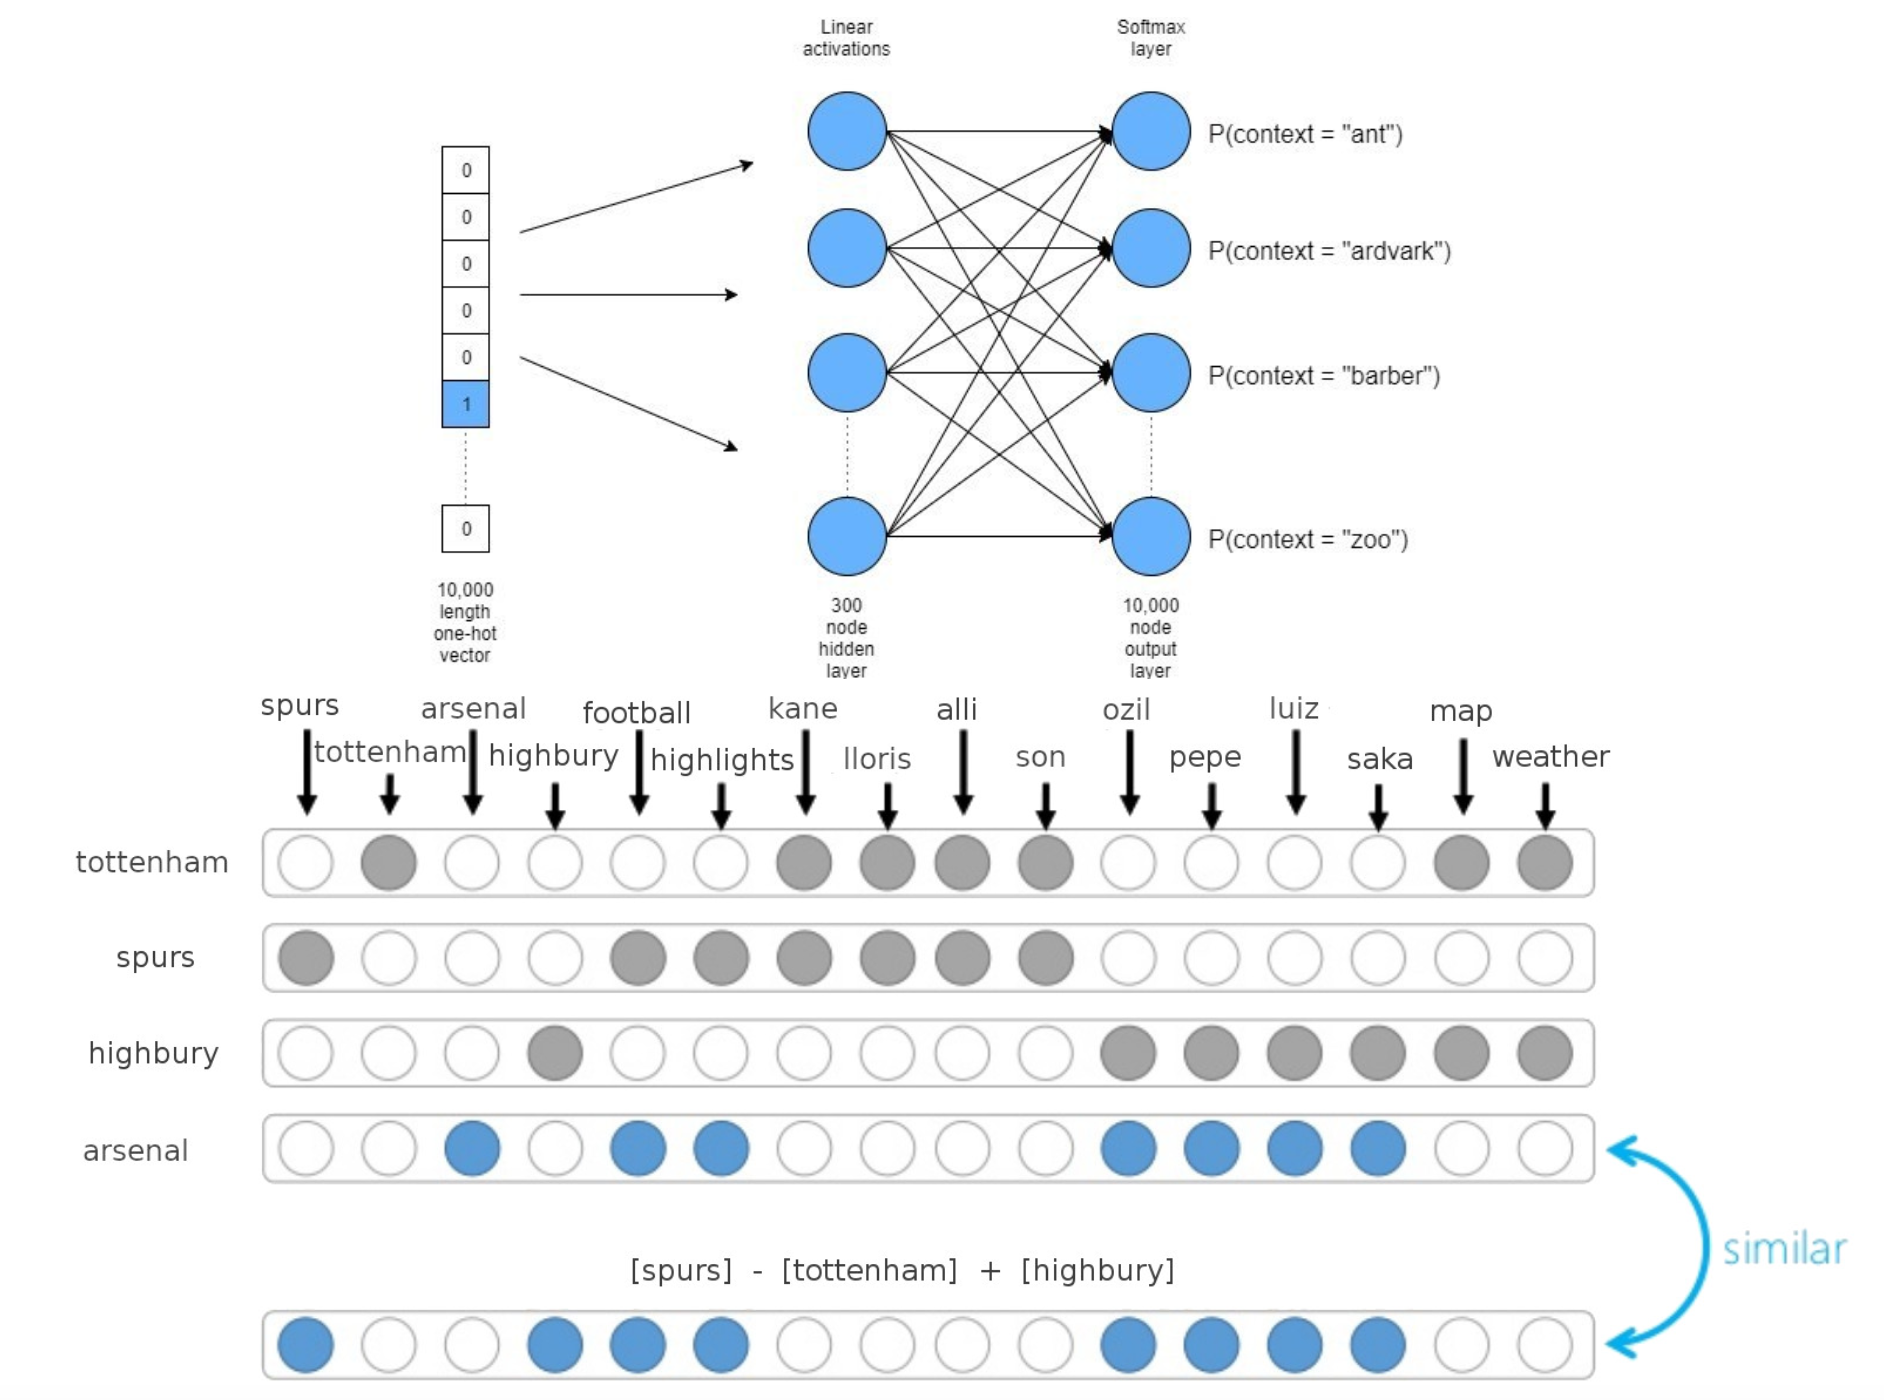
\includegraphics[width=0.75\linewidth]{img/w2v.png}
    \end{figure}

    \item \textbf{GloVe Embeddings: } GloVE, short for (Global Vectors for Word Representation) is an unsupervised learning algorithm for generating word embeddings.
    \begin{itemize}
        \item It uses global matrix factorisation techniques with a local context window to balance the focus between global statistics and local word co-occurrence.
        \item This helps GloVe capture both linear substructures and the semantics of word-word relationships within the corpus.
    \end{itemize}
    \begin{figure}[H]
        \centering
        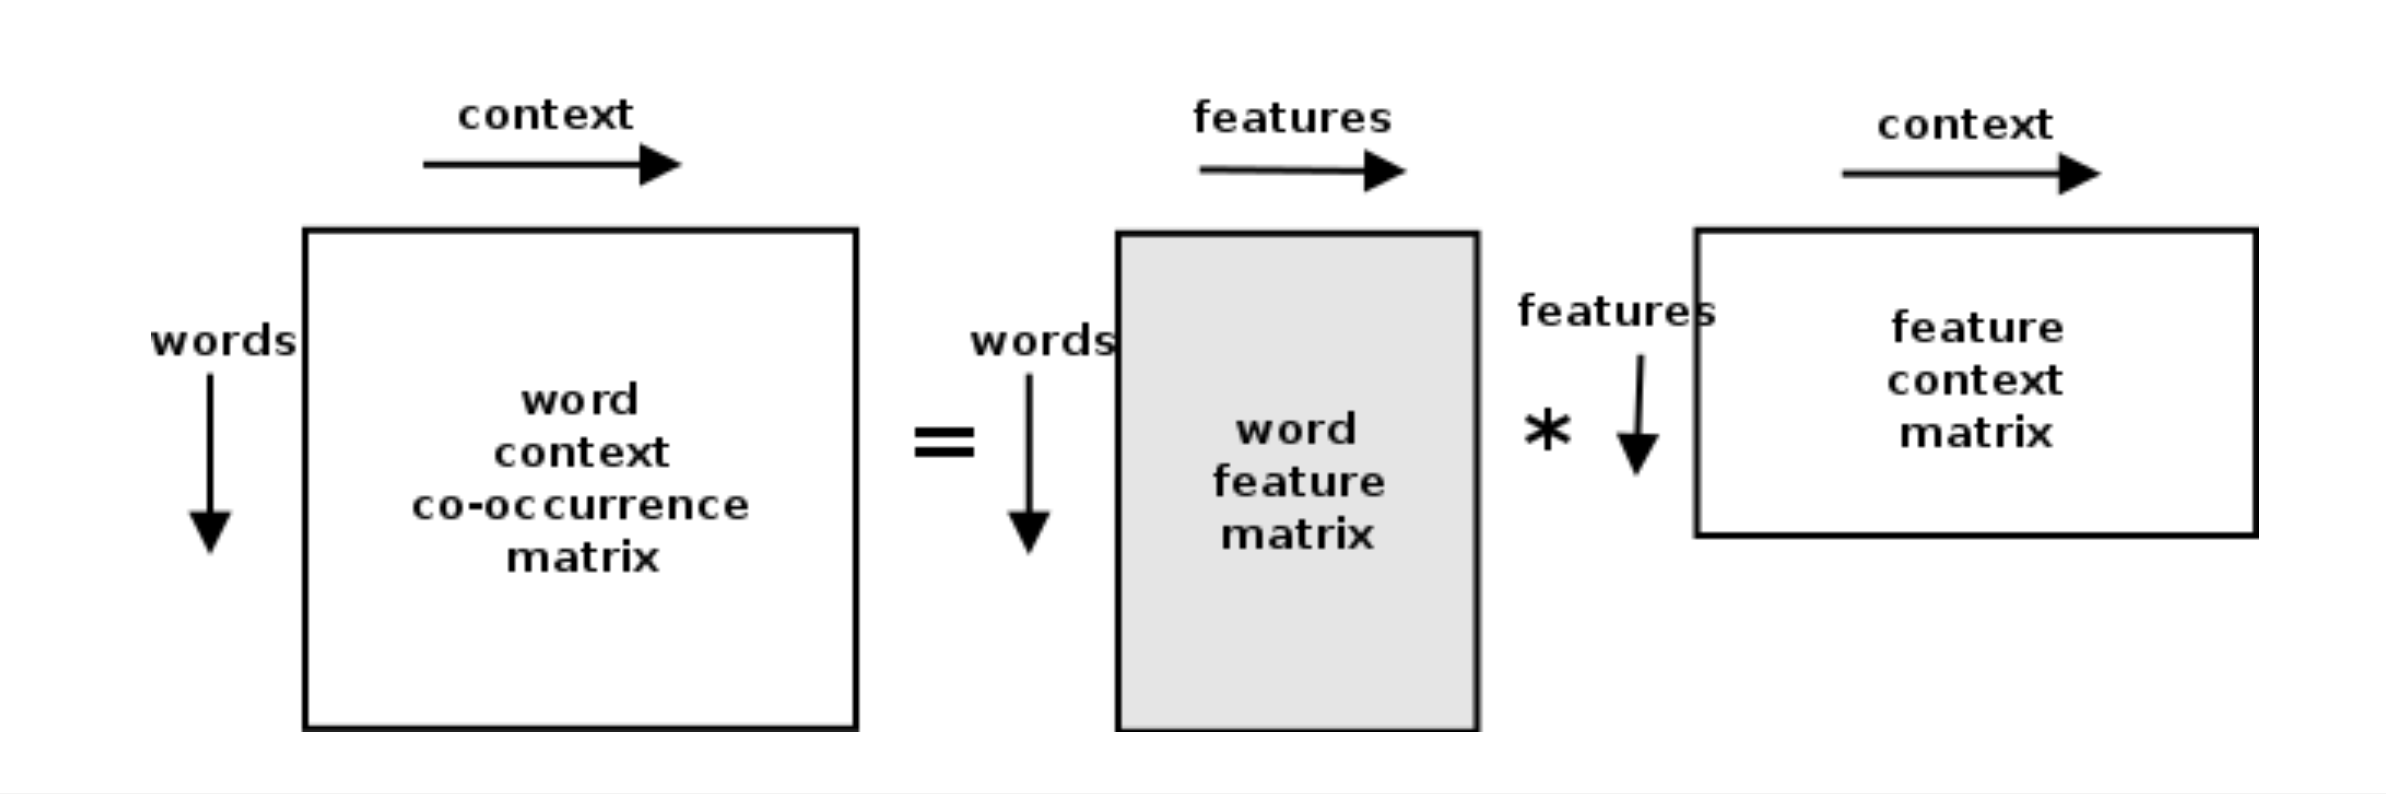
\includegraphics[width=0.75\linewidth]{img/glove.png}
        
    \end{figure}
\end{itemize}

\subsection{RNN Unit}
\begin{itemize}
    \item RNNs handle inputs $x_t \in \mathbb{R}^{N_{in}}$ and produce outputs $y_t \in \mathbb{R}^{N_{out}}$ for each timestep $t$.
    \item RNNs utilise a distributed hidden state, allowing them to store and process sequential information over time.
    \item They can be viewed as layered, feedforward networks with shared weights across the timesteps, which are trained using backpropagation through time (BPTT).
    \item During BPTT, gradients from all timesteps are accumulated for each weight, accounting for the shared weight structure.
    \item The hidden state $h_t \in \mathbb{R}^{N_h}$ is updated at each timestep according to:
    \begin{equation}
    h_t = \theta(W^{(hh)} h_{t-1} + W^{(xh)} x_t + b_h)
    \end{equation}
    where $\theta$ is a nonlinear activation function such as $\tanh$.
    \item The output $y_t$ is given by:
    \begin{equation}
    y_t = W^{(hy)} h_t + b_y
    \end{equation}
    with weight matrices:
    \begin{itemize}
        \item $W^{(hh)} \in \mathbb{R}^{N_h \times N_h}$
        \item $W^{(xh)} \in \mathbb{R}^{N_h \times N_{in}}$
        \item $W^{(hy)} \in \mathbb{R}^{N_{out} \times N_h}$
    \end{itemize}  and bias terms $b_h \in \mathbb{R}^{N_h}$, $b_y \in \mathbb{R}^{N_{out}}$.
    \item Outputs can also be fed back into the network as inputs for subsequent timesteps, e.g., $x_{t+1} = y_t$, to create a sequence-to-sequence model.
\end{itemize}

\begin{figure}[ht]
    \centering
    \begin{subfigure}[b]{0.4\textwidth}
        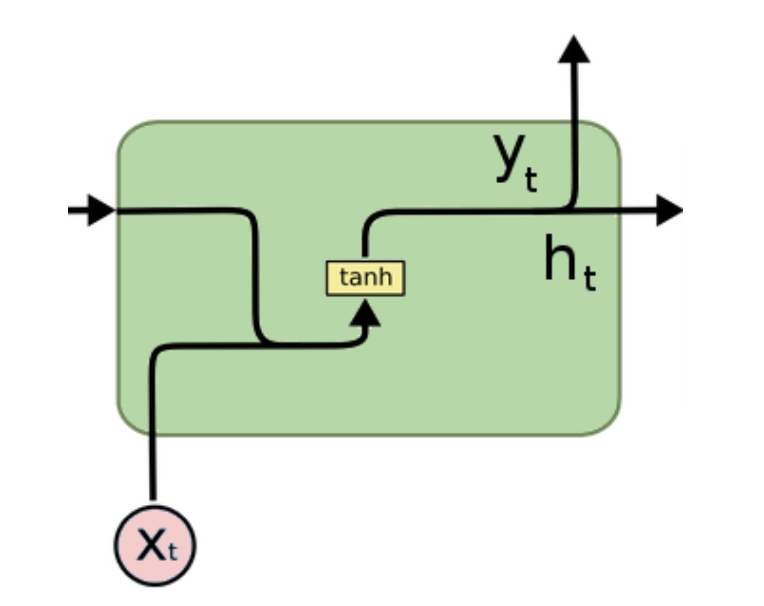
\includegraphics[width=\linewidth]{img/RNN_unit.png}
        \caption{A single RNN unit}
    \end{subfigure}
    \begin{subfigure}[b]{0.5\textwidth}
        \includegraphics[width=\linewidth]{img/RNN_structure.png}
        \caption{An RNN structure}
    \end{subfigure}
\end{figure}

\begin{itemize}

    \item RNNs are well-suited for modelling short-term dependencies due to the recurrent connections between hidden states.
    \item However, they often struggle with long-term dependencies because of the vanishing gradient problem, where gradients can become exponentially small as they propagate back through timesteps, leading to minimal weight updates and poor learning of long-range dependencies.
    \begin{equation}
        \delta^{(I)}=\left(\prod_{k=I}^{L-1}\theta^{\prime}(s^{(k)})(W^{(k)})^T\right)\theta^{\prime}(s^{(L)})\nabla_{x^{(L)}}\mathcal{L}
    \end{equation}
\end{itemize}


\begin{figure}[H]
    \centering
    

\end{figure}
\break
\subsection{Long Short Term Memory}
LSTM units are designed to address the long-term dependency problem present in traditional RNNs by incorporating mechanisms that allow for preserving information over extended periods.
\begin{figure}[H]
    \centering
    \begin{subfigure}[b]{0.45\textwidth}
        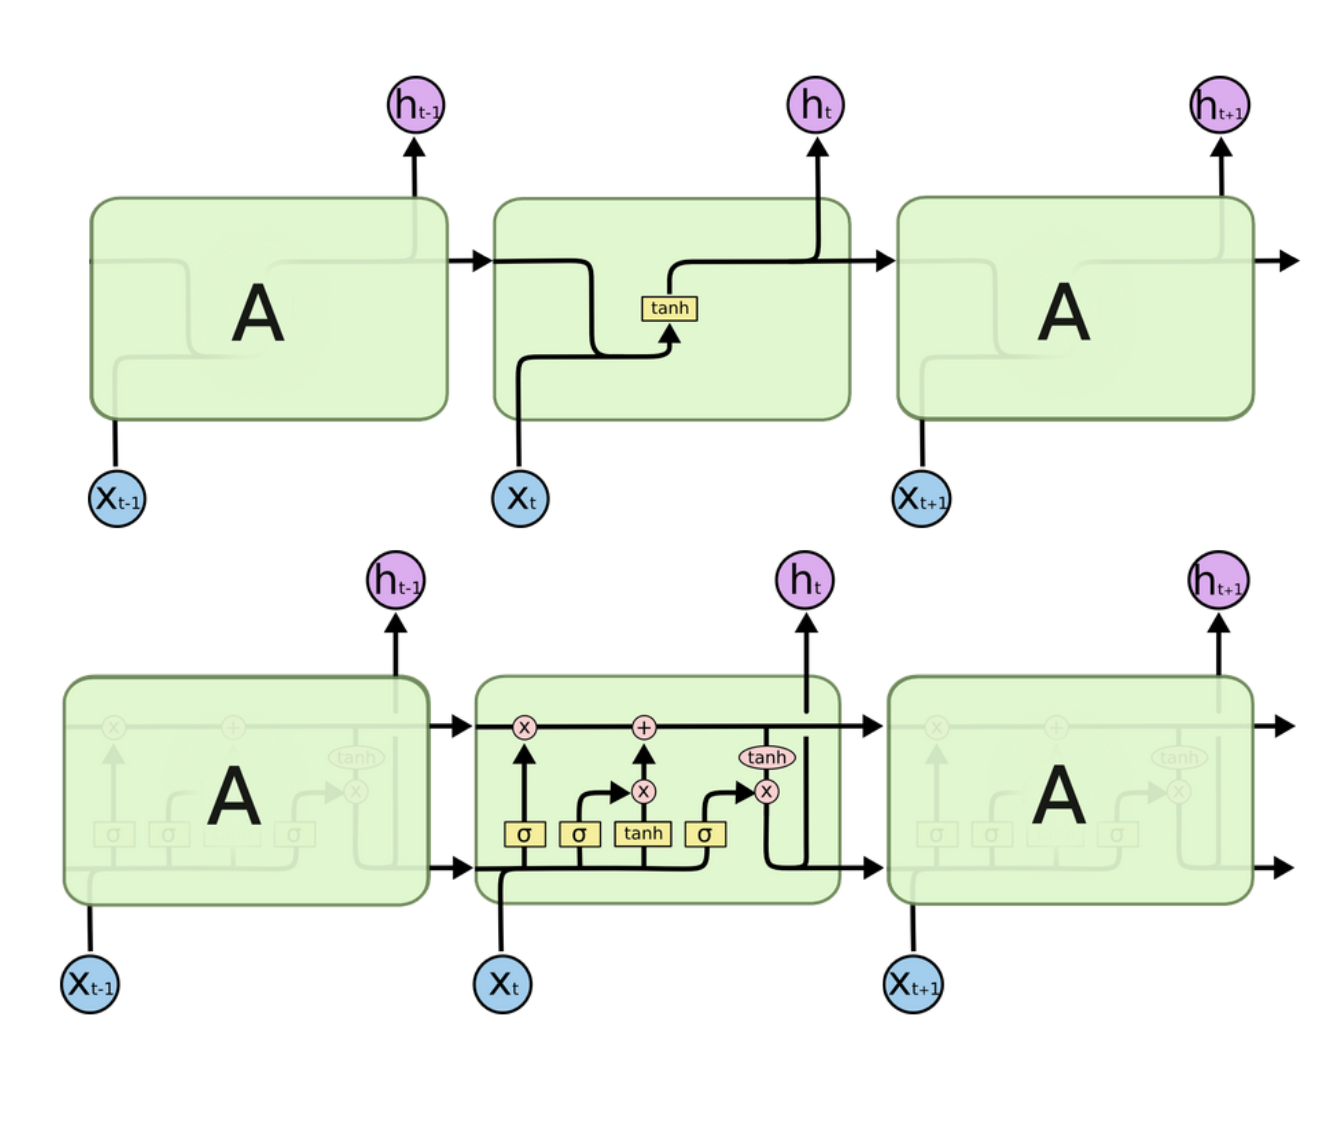
\includegraphics[width=\linewidth]{img/LSTM.png}
        \caption{LSTM units diagram}
    \end{subfigure}
    \begin{subfigure}[b]{0.30\textwidth}
        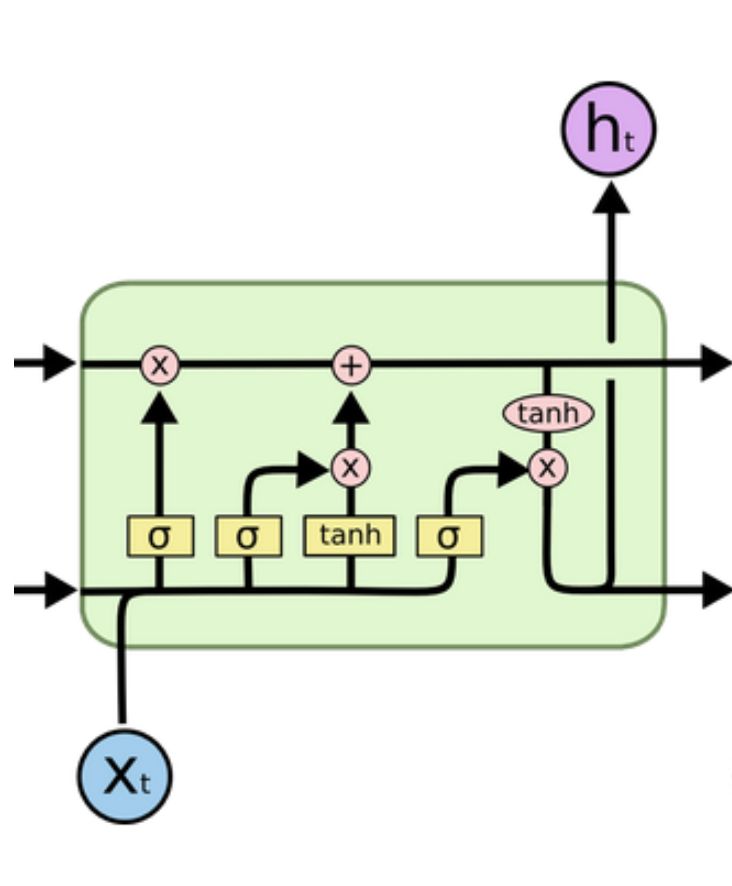
\includegraphics[width=\linewidth]{img/LSTM_closeup.png}
        \caption{LSTM unit close-up}
    \end{subfigure}
\end{figure}

\begin{figure}[H]
    \centering
    \begin{subfigure}[b]{0.4\textwidth}
        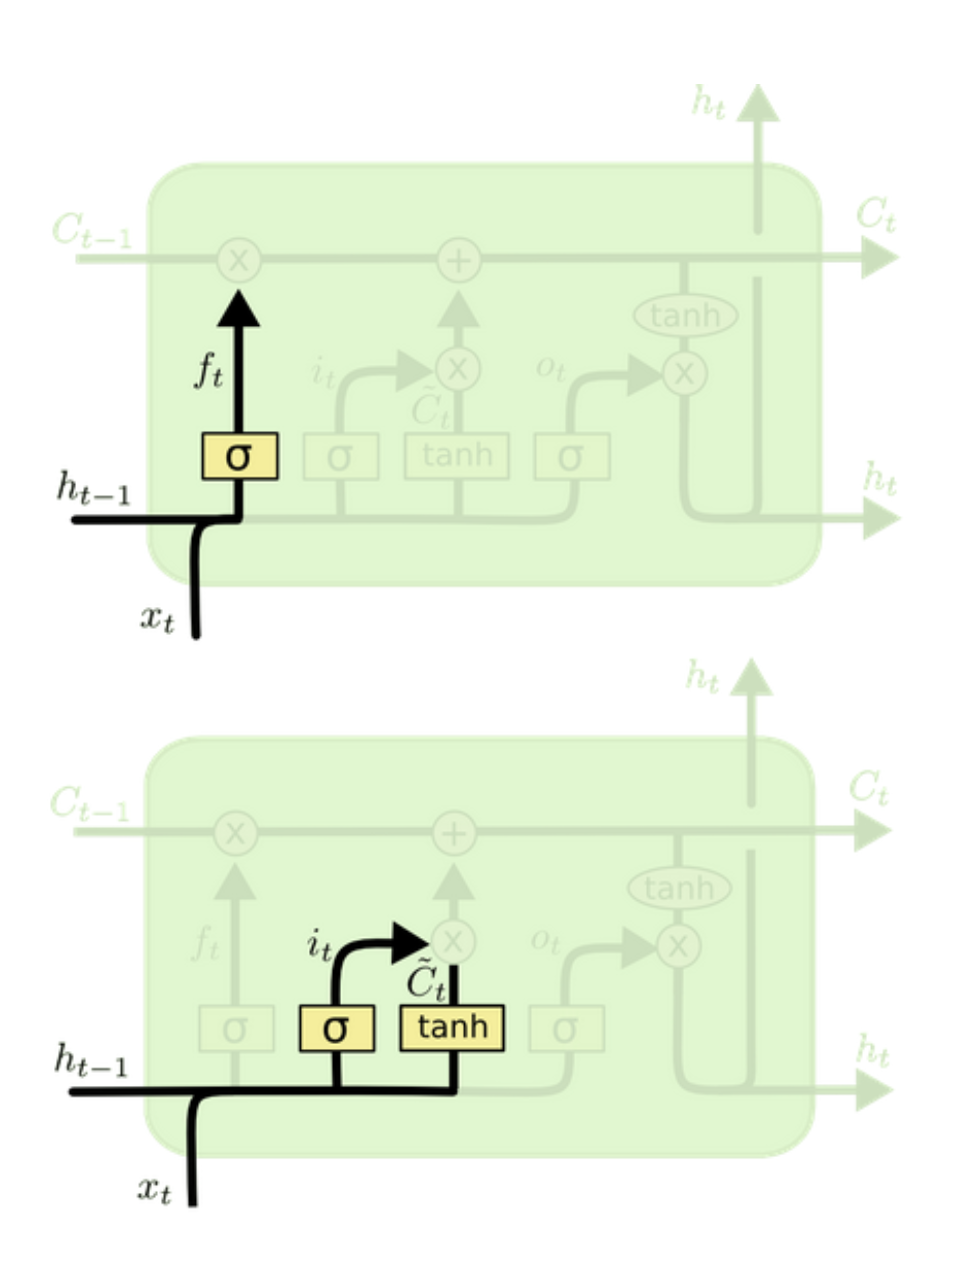
\includegraphics[width=\linewidth]{img/LSTM_unit.png}
        \caption{Forget Gate $f_t$ and Update Gate $i_t$}
    \end{subfigure}
    \begin{subfigure}[b]{0.4\textwidth}
        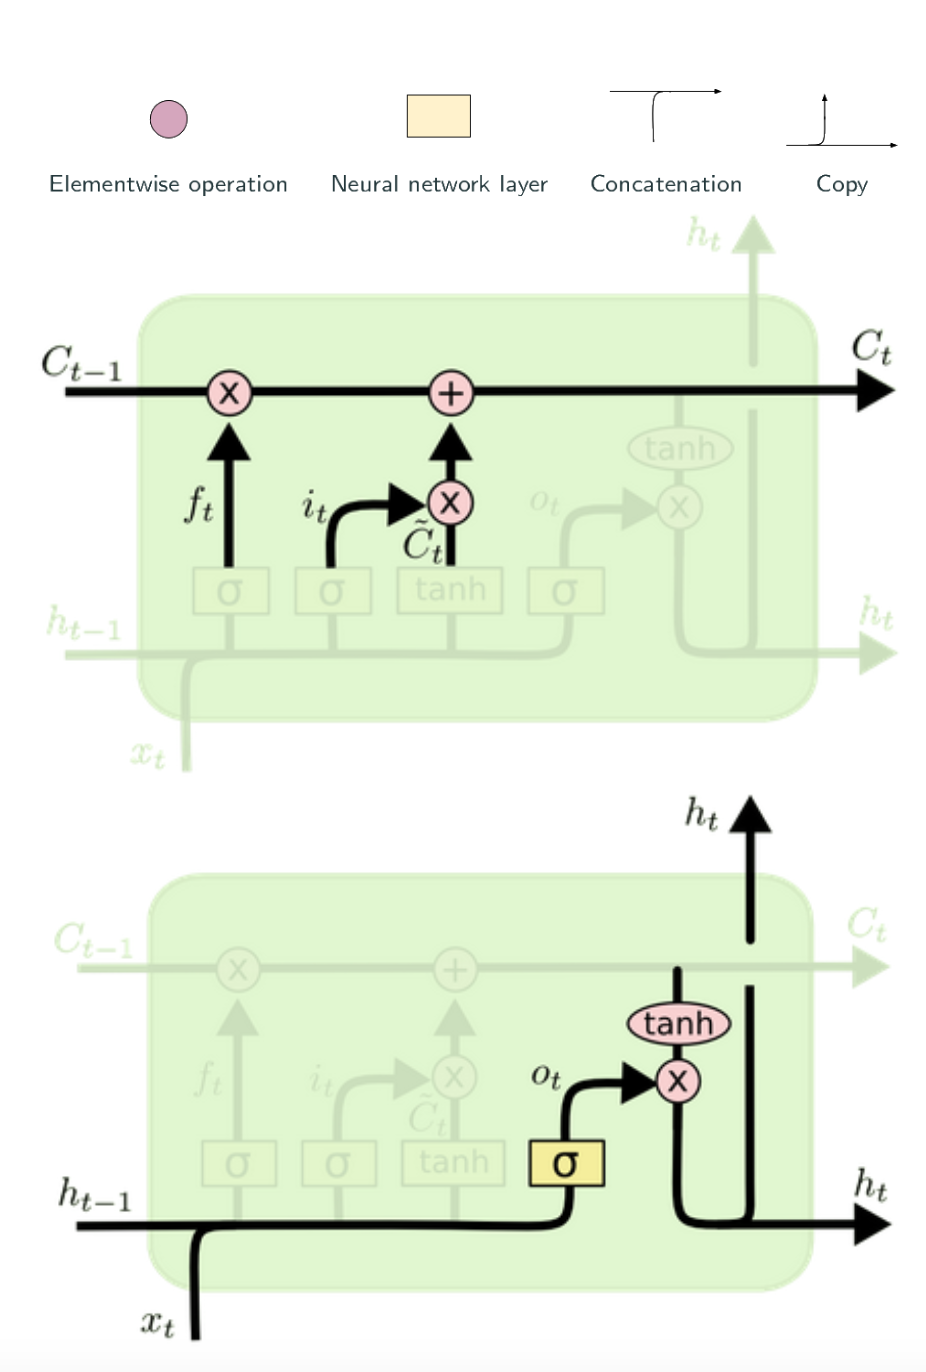
\includegraphics[width=\linewidth]{img/LSTM_unit_learn.png}
        \caption{Internal cell state $C_t$ and Output Gate $0_t$}
    \end{subfigure}
\end{figure}


\begin{itemize}
    \item LSTMs consist of multiple layers with three sigmoid gates (forget, input/update, and output) that regulate the flow of information. These gates determine what information is retained or discarded at each timestep.
    \item The \textit{forget gate} \( f_t \) decides which portions of the previous state to retain: (We denote $\sigma$ as sigmoid activation function for this diagram)
    \begin{equation*}
        f_t = \sigma(W_f [h_{t-1}, x_t] + b_f)
    \end{equation*}
    \item The \textit{update gate} \( i_t \) and the \textit{interal cell state} \( \tilde{C}_t \) decide what new information to store in the cell state:
    \begin{equation*}
        i_t = \sigma(W_i [h_{t-1}, x_t] + b_i)
    \end{equation*}
    \begin{equation*}
        \tilde{C}_t = \tanh(W_C [h_{t-1}, x_t] + b_C)
    \end{equation*}
    \item The \textit{cell state} \( C_t \) is updated as an elementwise combination of the old state and new candidate state, modulated by the forget and input gates (denote $\oplus$ as element-wise addition and $\otimes$ as element-wise multiplication):
    \begin{equation*}
        C_t = f_t \otimes C_{t-1} \oplus i_t \otimes \tilde{C}_t
    \end{equation*}
    \item The \textit{output gate} \( o_t \) decides what part of the cell state to output:
    \begin{equation*}
        o_t = \sigma(W_o [h_{t-1}, x_t] + b_o)
    \end{equation*}
    \begin{equation*}
        h_t = o_t \otimes \tanh(C_t)
    \end{equation*}
\end{itemize}




\subsection{Pros and Cons of Typical RNN Architecture}
\subsubsection*{Advantages of RNNs}
\begin{itemize}
    \item Capable of processing inputs of any length, allowing for flexibility in handling sequences.
    \item The model size remains constant and does not increase with the size of input, making the architecture scalable.
    \item Computation accounts for historical information, enabling the network to use the context from previous inputs.
    \item Weights are shared across time, reducing the number of parameters and computational load.
\end{itemize}

\subsubsection*{Drawbacks of RNNs}
\begin{itemize}
    \item Computationally intensive, especially for long sequences, leading to slower training and inference times.
    \item Difficulty in accessing information from early in the sequence due to vanishing gradient issues, affecting long-term dependencies.
    \item Inability to consider any future input for the current state as the computation is sequential and based only on past information.
    \item The number of internal parameters can still be large, demanding significant computational resources.
\end{itemize}

\subsection{Gated Recurrent Unit}
\begin{figure}[H]
    \centering
    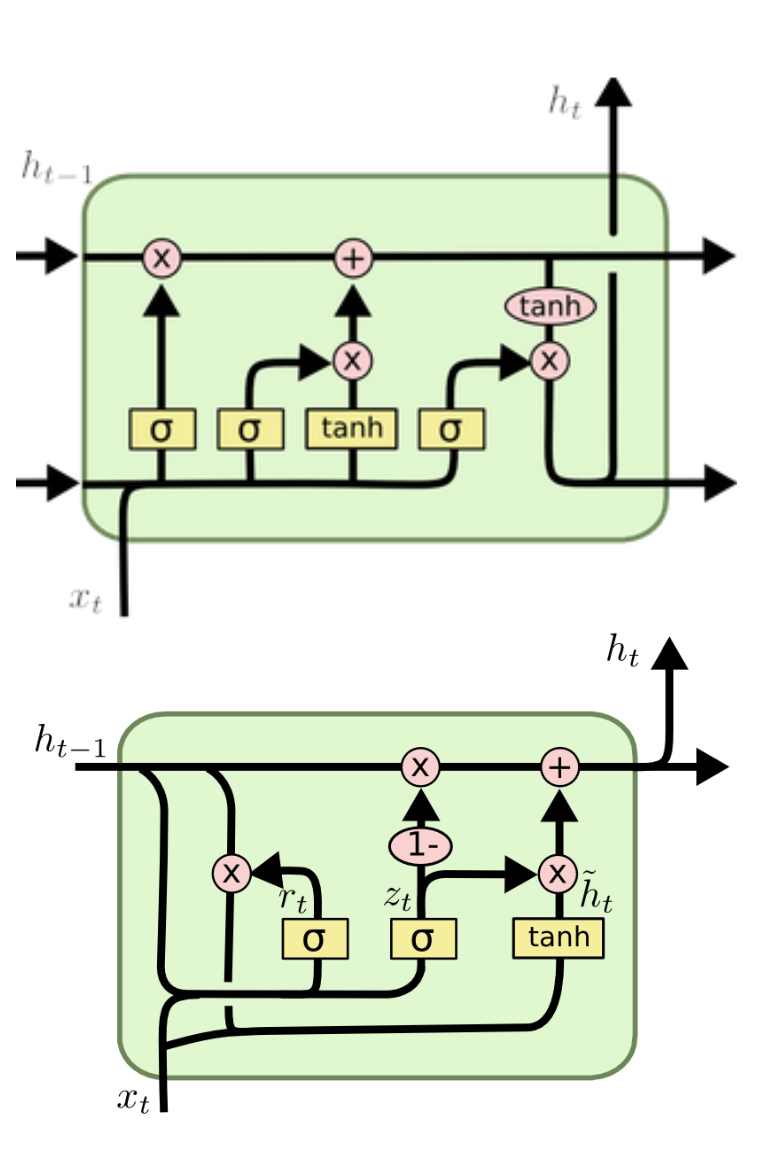
\includegraphics[width=0.4\linewidth]{img/GRU.png}
    
\end{figure}

\begin{itemize}
    \item GRUs adaptively reset and update memory with two gates, \( r_t \) and \( z_t \), analogous to the forget and input gates of the LSTM.
    \begin{align*}
        z_t &= \sigma(W_z [h_{t-1}, x_t] + b_z) \\
        r_t &= \sigma(W_r [h_{t-1}, x_t] + b_r) \\
        \hat{h}_t &= \tanh(W [r_t \otimes h_{t-1}, x_t] + b) \\
        h_t &= (1 - z_t) \otimes h_{t-1} \oplus z_t \otimes \hat{h}_t \\
        o_t &= h_t
    \end{align*}
    \item GRU fully exposes its memory at each timestep, simplifying the structure compared to LSTM which has separate memory cells.
    \item The output is a combination of the last state and the new candidate state, providing a combination of historical and current information.
    \item While LSTM and GRU both outperform traditional tanh units, empirical studies show marginal performance differences between them.
\end{itemize}


\section{LSTM architectures}


\subsection{Bidirectional RNNs and Deep RNNs }

\subsubsection*{Bidirectional Recurrent Neural Networks (BRNNs)}
\begin{itemize}
    \item BRNNs are designed to process sequences by considering both past (backward) and future (forward) contexts. It processes an input sequence in both directions with two separate hidden states, which are typically combined through concatenation or summation.
    \item The dual processing streams allow the network to capture dependencies and patterns that span across the entire input sequence, enhancing its predictive capabilities.
    \item This architecture is particularly effective for sequence-to-sequence learning tasks such as language translation and speech recognition.
    \item In language modelling, like with ELMO and Google Translate, BRNNs can significantly enhance the context-awareness of the model, leading to improved performance over unidirectional approaches.

\end{itemize}

\subsubsection*{Deep Recurrent Neural Networks (DRNNs)}
\begin{itemize}
    \item DRNNs feature multiple layers of RNNs stacked on top of each other, with the output sequence of one layer forming the input sequence for the next.
    \item This depth enables the network to learn a hierarchy of features at different levels of abstraction, making it suitable for complex tasks with large datasets such as video processing.
    \item Deep architectures can model complex temporal dynamics due to the increased representational power provided by the additional layers.
    \item Each layer captures different features of the sequence, with higher levels potentially learning more abstract representations of the data.
    \item Despite their power, DRNNs can be challenging to train effectively due to issues such as vanishing or exploding gradients, which are mitigated using techniques like LSTM or GRU cells.
\end{itemize}

Both BRNNs and DRNNs are advancements in neural network design to improve the handling of sequential data, with applications in natural language processing, speech synthesis, and video analysis. Both models can consider the broader context and learn deep representations enabling them to capture complex patterns and relationships within data.


\begin{figure}[H]
    \centering
    \begin{subfigure}[b]{0.45\textwidth}
        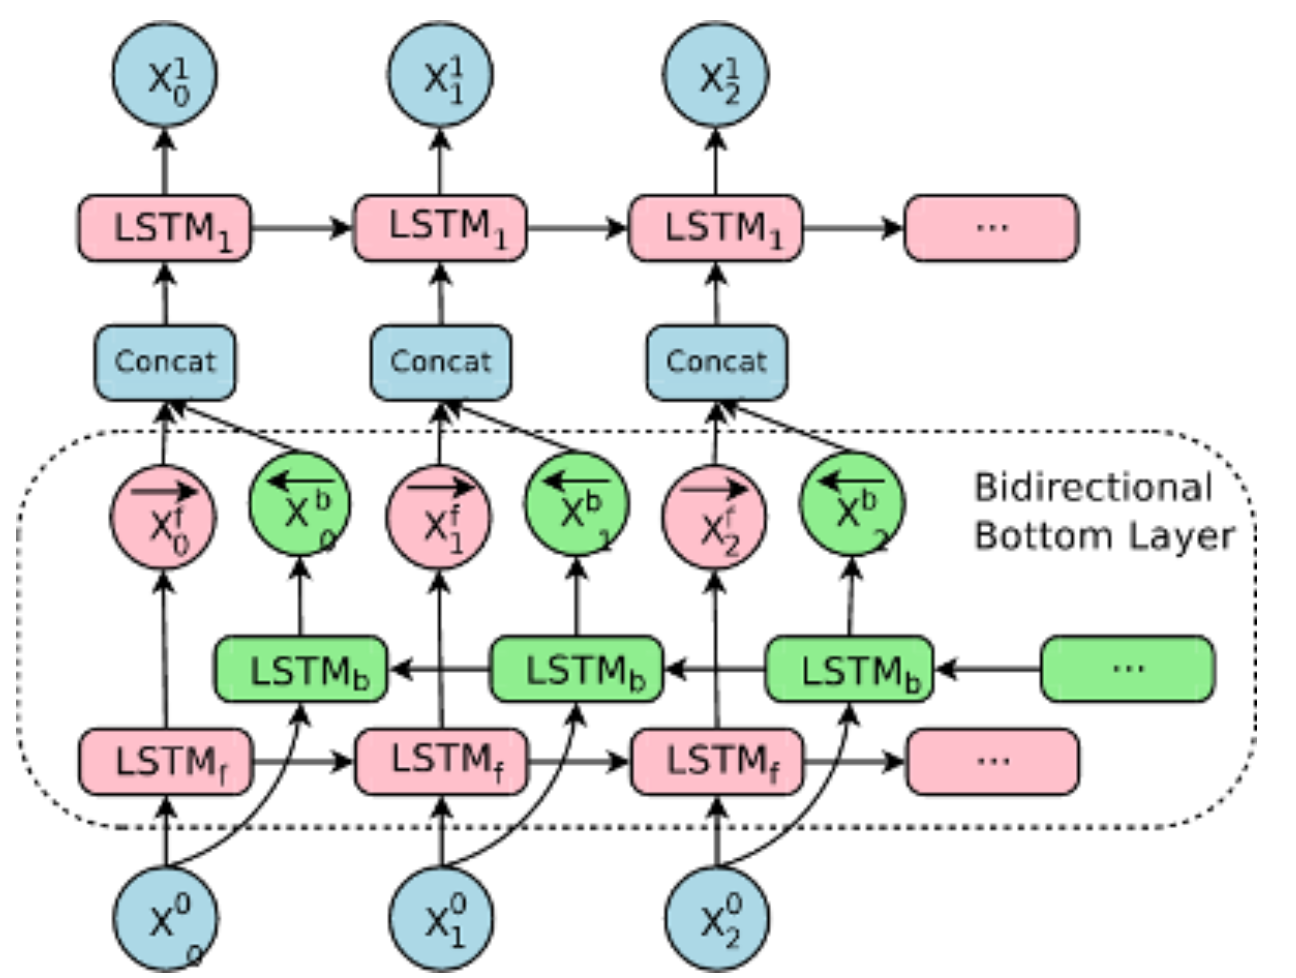
\includegraphics[width=\linewidth]{img/BRNN.png}
        \caption{BRNN model}
    \end{subfigure}
    \begin{subfigure}[b]{0.30\textwidth}
        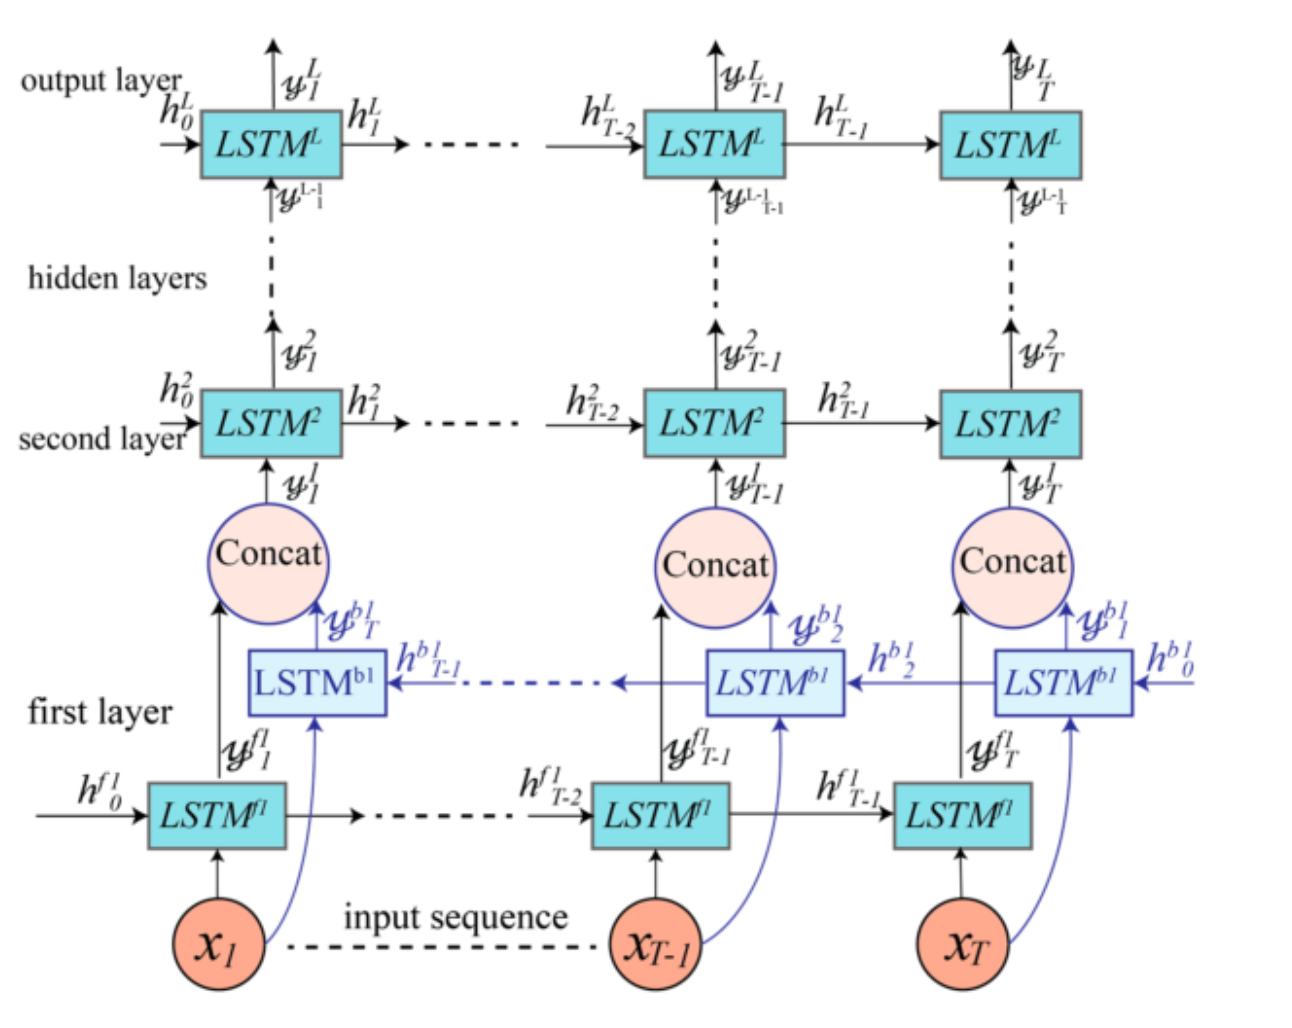
\includegraphics[width=\linewidth]{img/DRNNs.png}
        \caption{DRNN with many hidden layers}
    \end{subfigure}
\end{figure}
\subsection{Input-Output Types and Applications}
\begin{figure}[H]
    \centering
    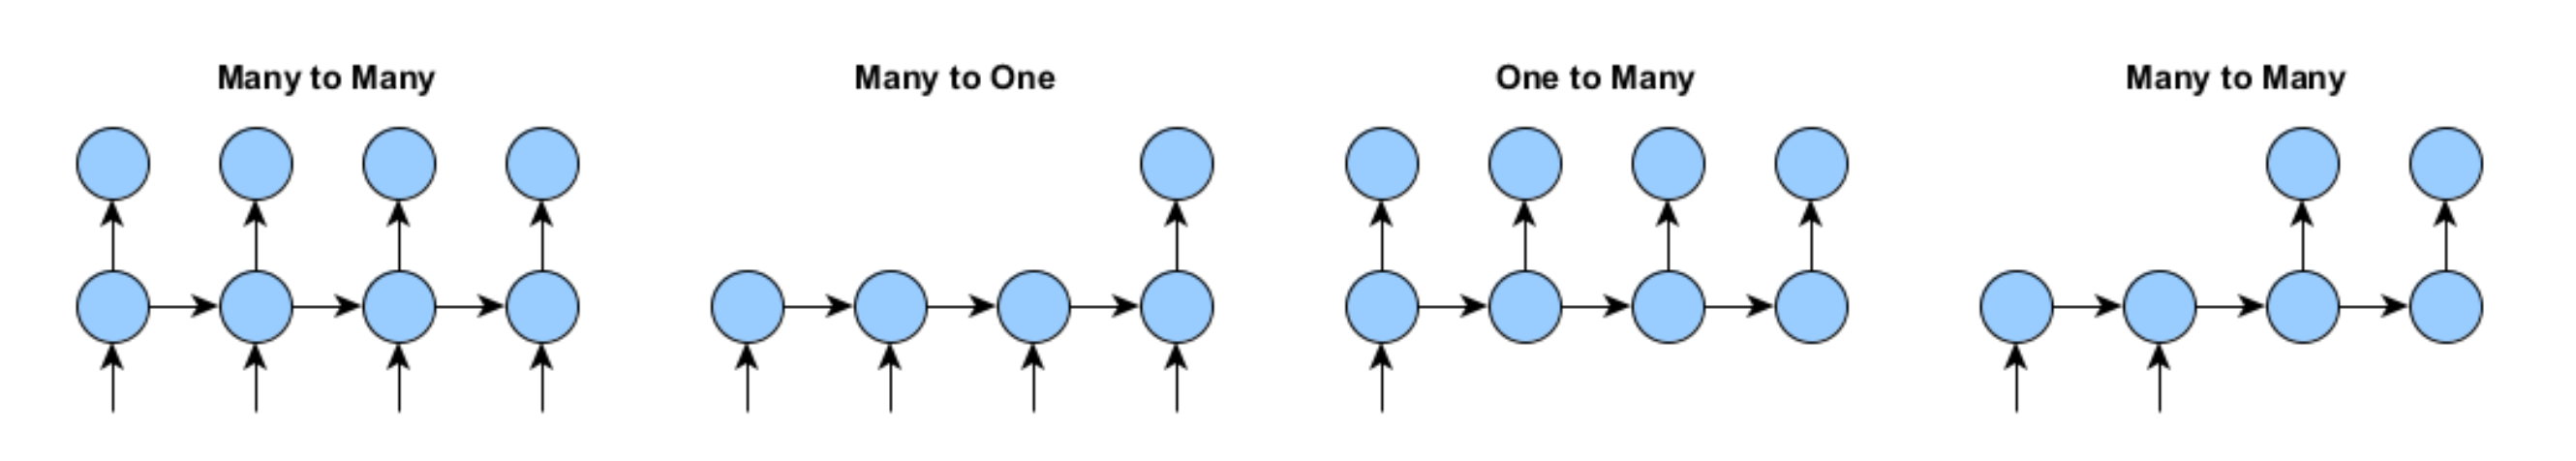
\includegraphics[width=0.75\linewidth]{img/LSTMs_IO.png}
\end{figure}

\subsubsection{Many to Many}
\begin{itemize}
    \item For use with with temporal data input and output
    \item Speech recognition: audio sequence input, text sequence output
    \item Video annotation: video input and text output
    \begin{figure}[H]
        \centering
        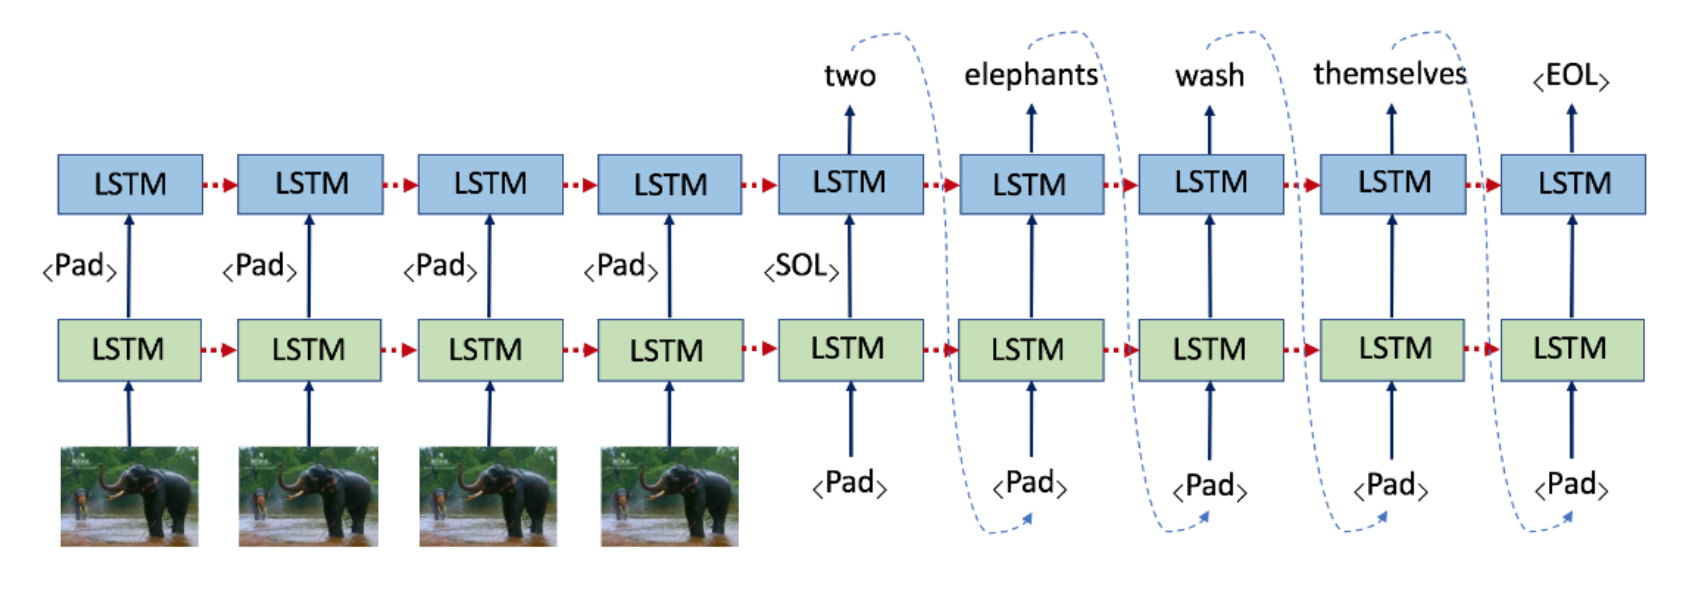
\includegraphics[width=0.75\linewidth]{img/vid_annotation.png}
    \end{figure}
    \item Language Translation: The encoder RNN encodes entire source sentence into the final hidden state. Although it is difficult to store long sentences in the state.
    \begin{figure}[H]
        \centering
        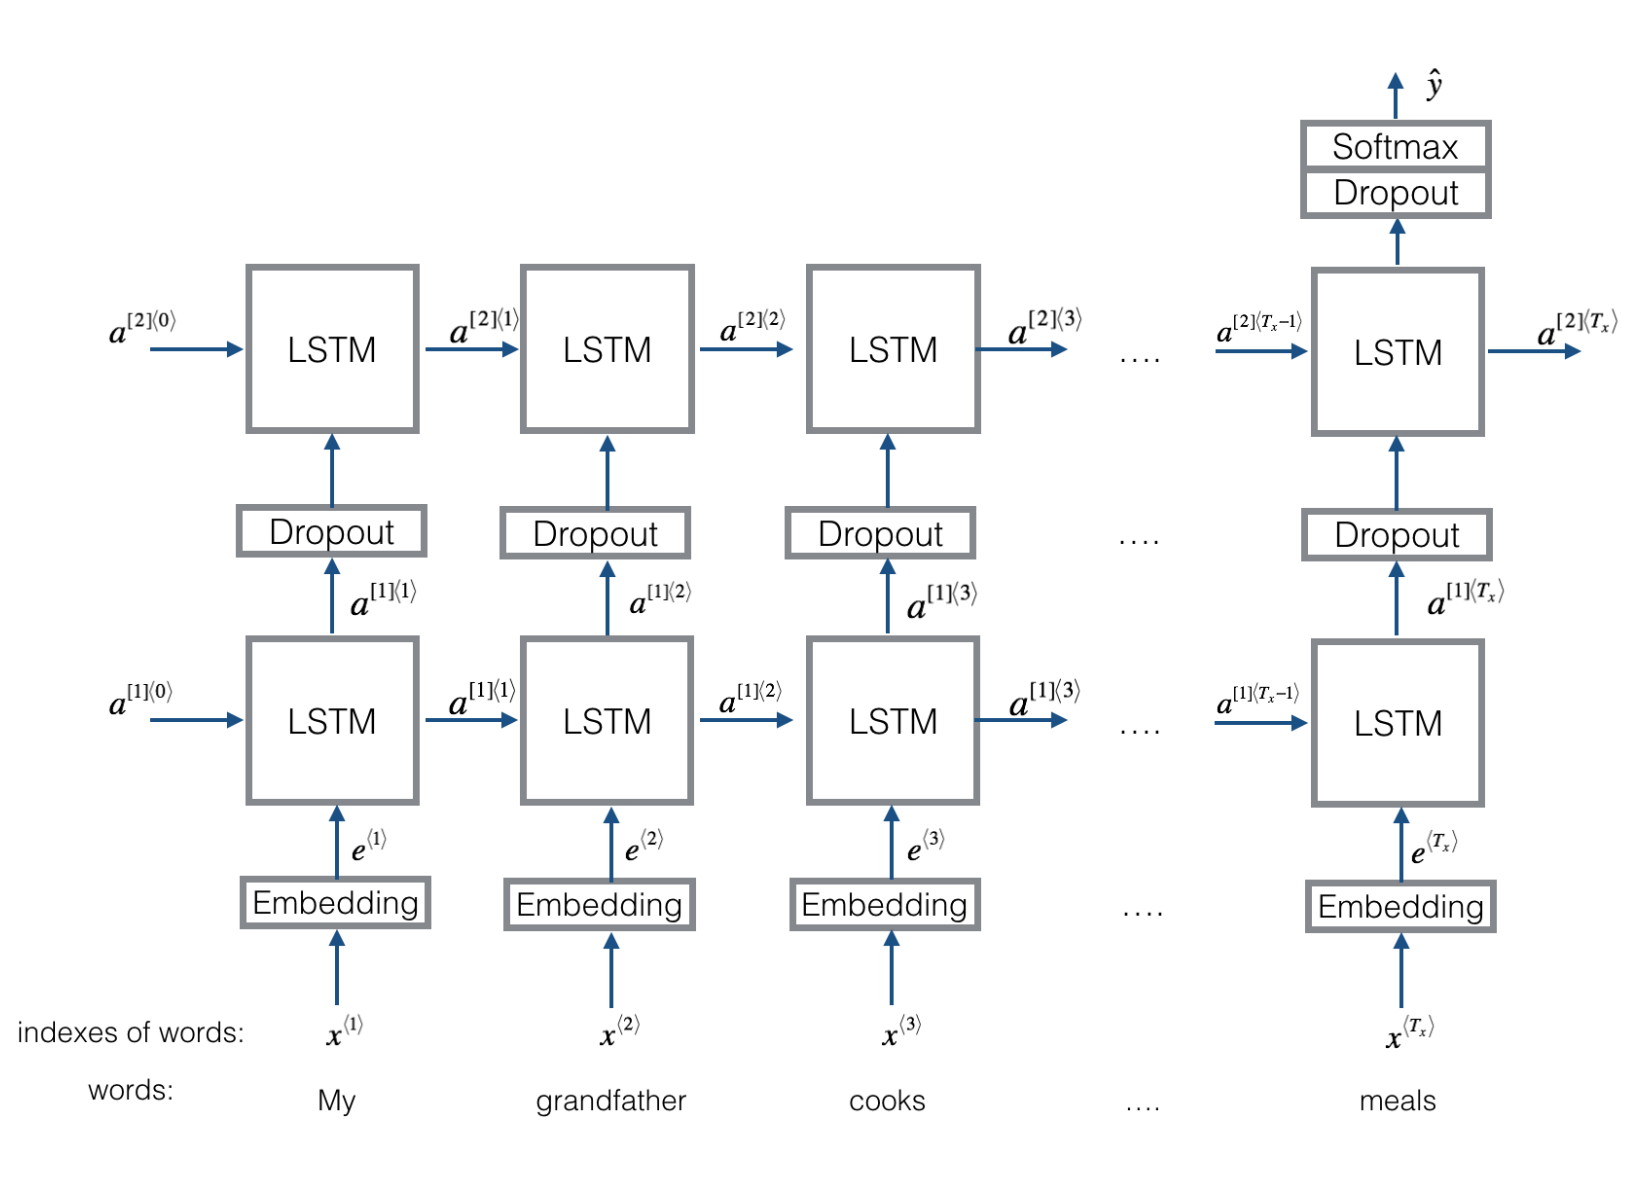
\includegraphics[width=0.75\linewidth]{img/translate.png}

    \end{figure}

    
\end{itemize}
\subsubsection{Many to One}
\begin{itemize}
    \item Temporal data input, simple output (classification for sentiment analysis)
    \item Sentiment Analysis: a sentence (multiple words) is input into the multi-layer LSTM, and outputs a probability between positive or negative sentiment. Dropout used for regularisation
    \begin{figure}[H]
        \centering
        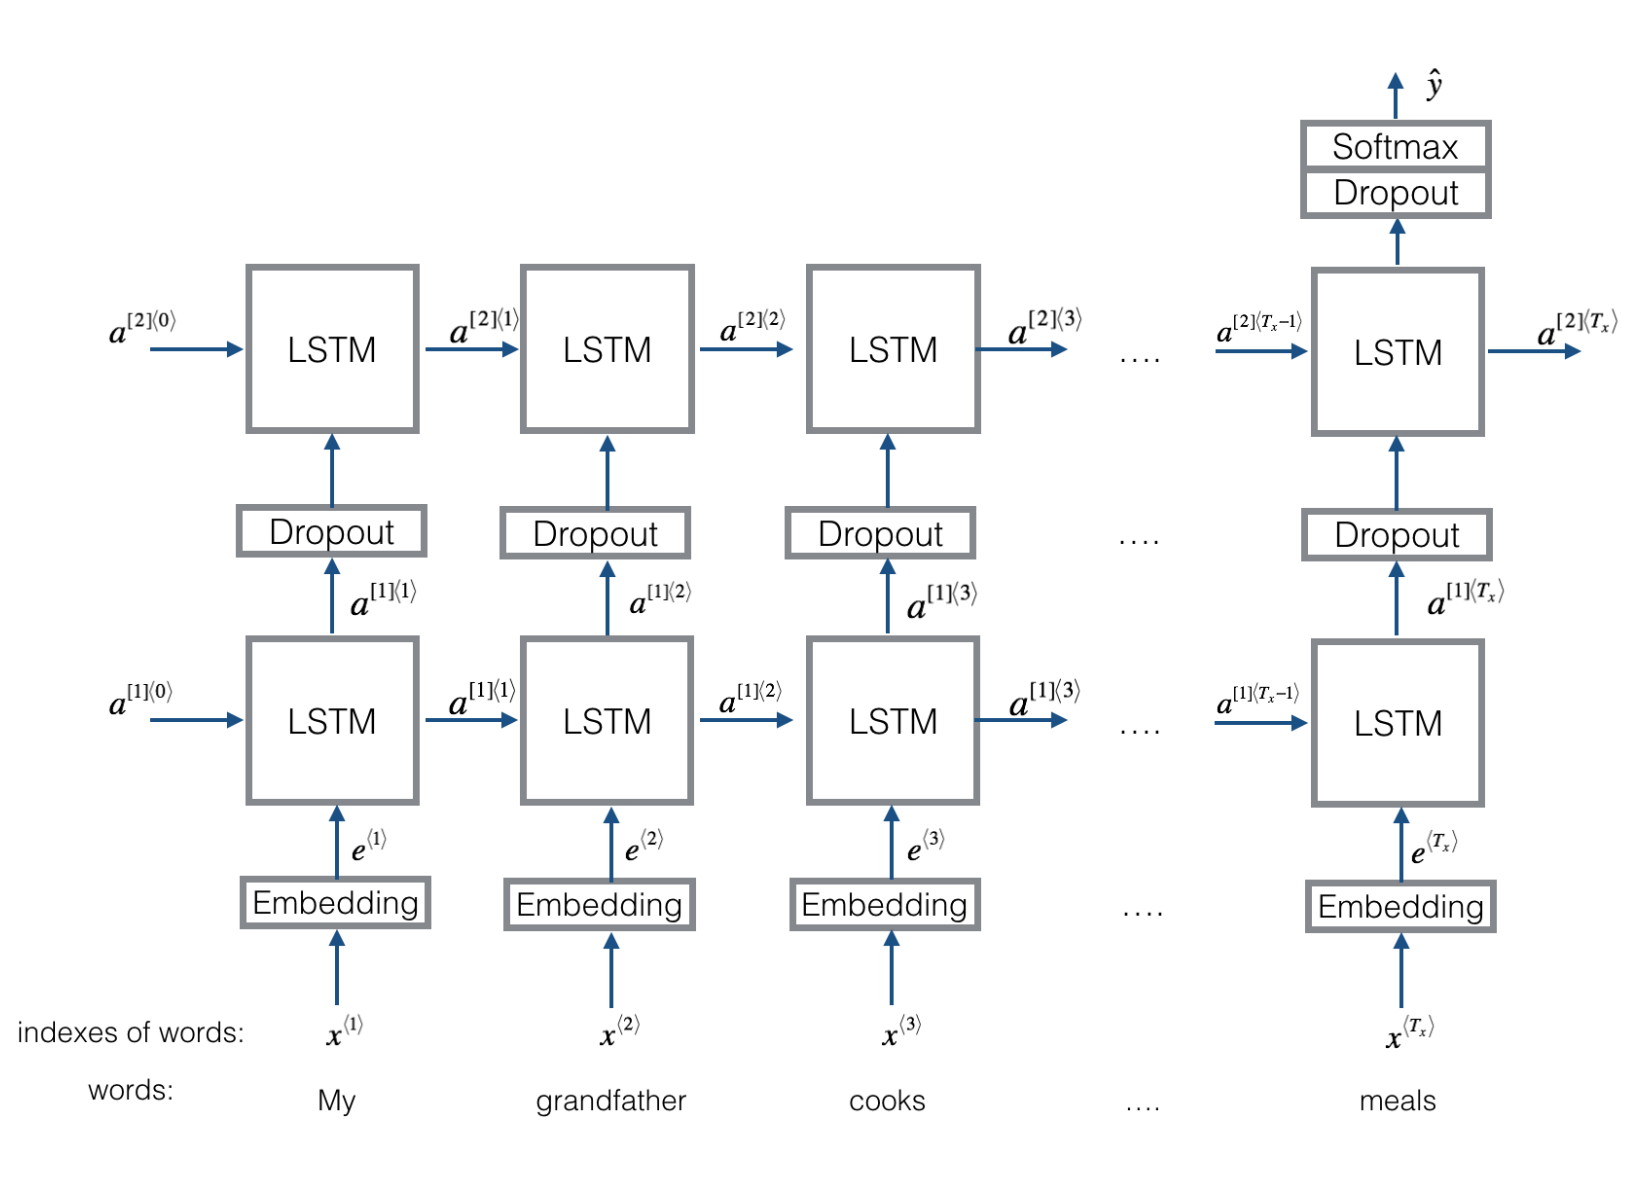
\includegraphics[width=0.65\linewidth]{img/sentiment_analysis.png}
    \end{figure}
\end{itemize}
\subsubsection{One to Many}
\begin{itemize}
    \item Simple input, temporal data output.
    \item Image captioning: Single image input, sentence (multiple words) output
    \begin{figure}[H]
        \centering
        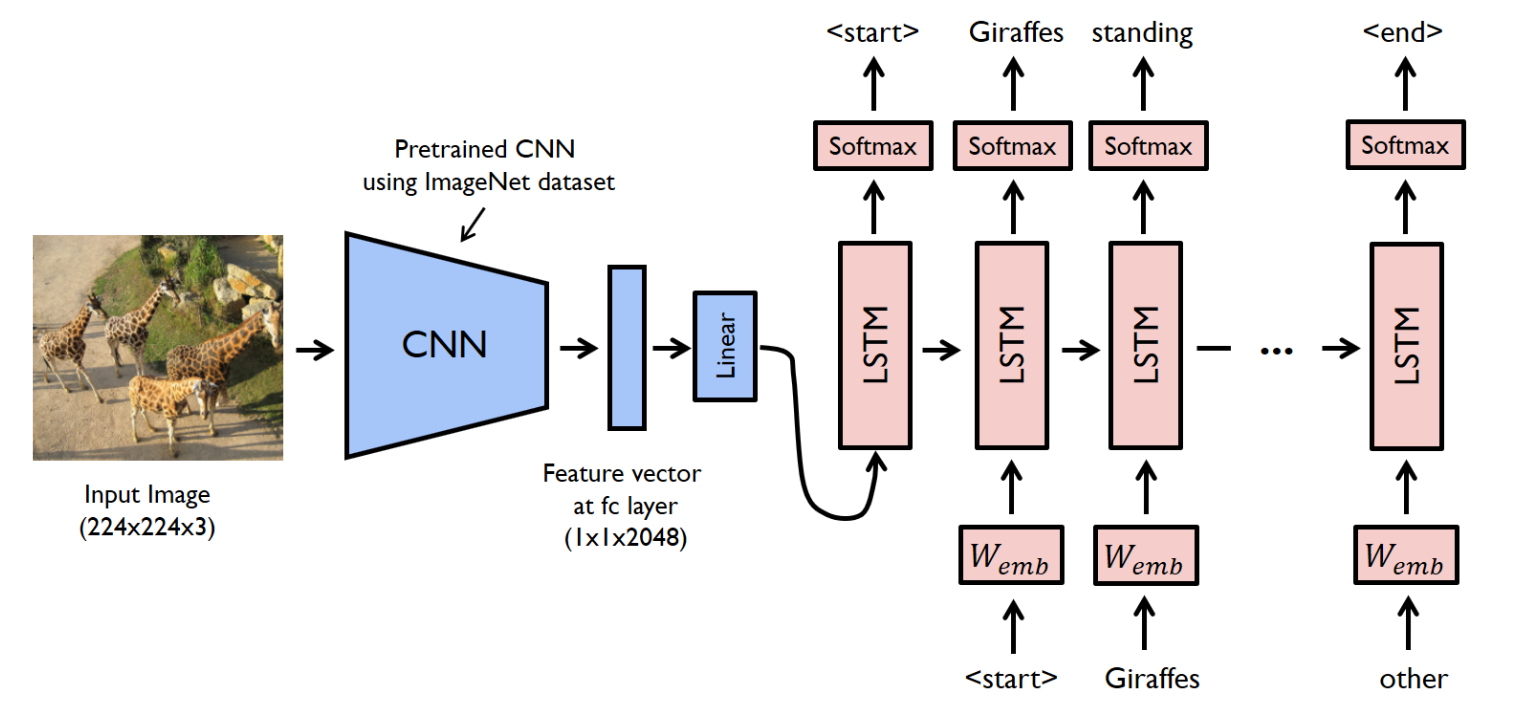
\includegraphics[width=0.75\linewidth]{img/lstm_image_captioning.png}
    \end{figure}
    \item Audio generation: Training an LSTM on a dataset of music to produce its own, correcting it with music theory (structuring it for human hearing and preference), and training again with generated + the dataset, will allow it to produce machine created music. Generation only = one to many.
\end{itemize}


\section{Attention Mechanism in LSTMs}
\begin{itemize}
    \item Attention mechanisms enable neural networks network to focus on specific parts of the input sequence when performing a task, mimicking the ability to pay attention selectively to the most relevant information.
    \item During the decoding phase of sequence translation, the attention mechanism allows the decoder to consider different segments of the source sentence at each step, thereby aligning the output sequence more accurately with the input.
    \item An alignment model calculates attention scores by comparing the most recent hidden state of the decoder with each hidden state of the encoder. These scores determine how much focus to put on different parts of the input sequence.
    \item Mathematically, the hidden state sequence \( h_t \) is transformed by a learnable attention layer \( a(h_t) \), typically using a softmax function to output a probability vector \( \alpha \), which signifies the degree of attention or weight given to each encoder state.
    \item The context vector \( c \) is computed as a weighted sum of the encoder hidden states:
    \begin{equation*}
        c = \sum_{t} (\alpha_t \otimes h_t)
    \end{equation*}
    \item This context vector \( c \) is then used in combination with the decoder's own hidden state to generate the next element of the output sequence. The use of attention ensures that the network's outputs are conditioned more accurately on relevant input information.
\end{itemize}

\begin{figure}[H]
    \centering
    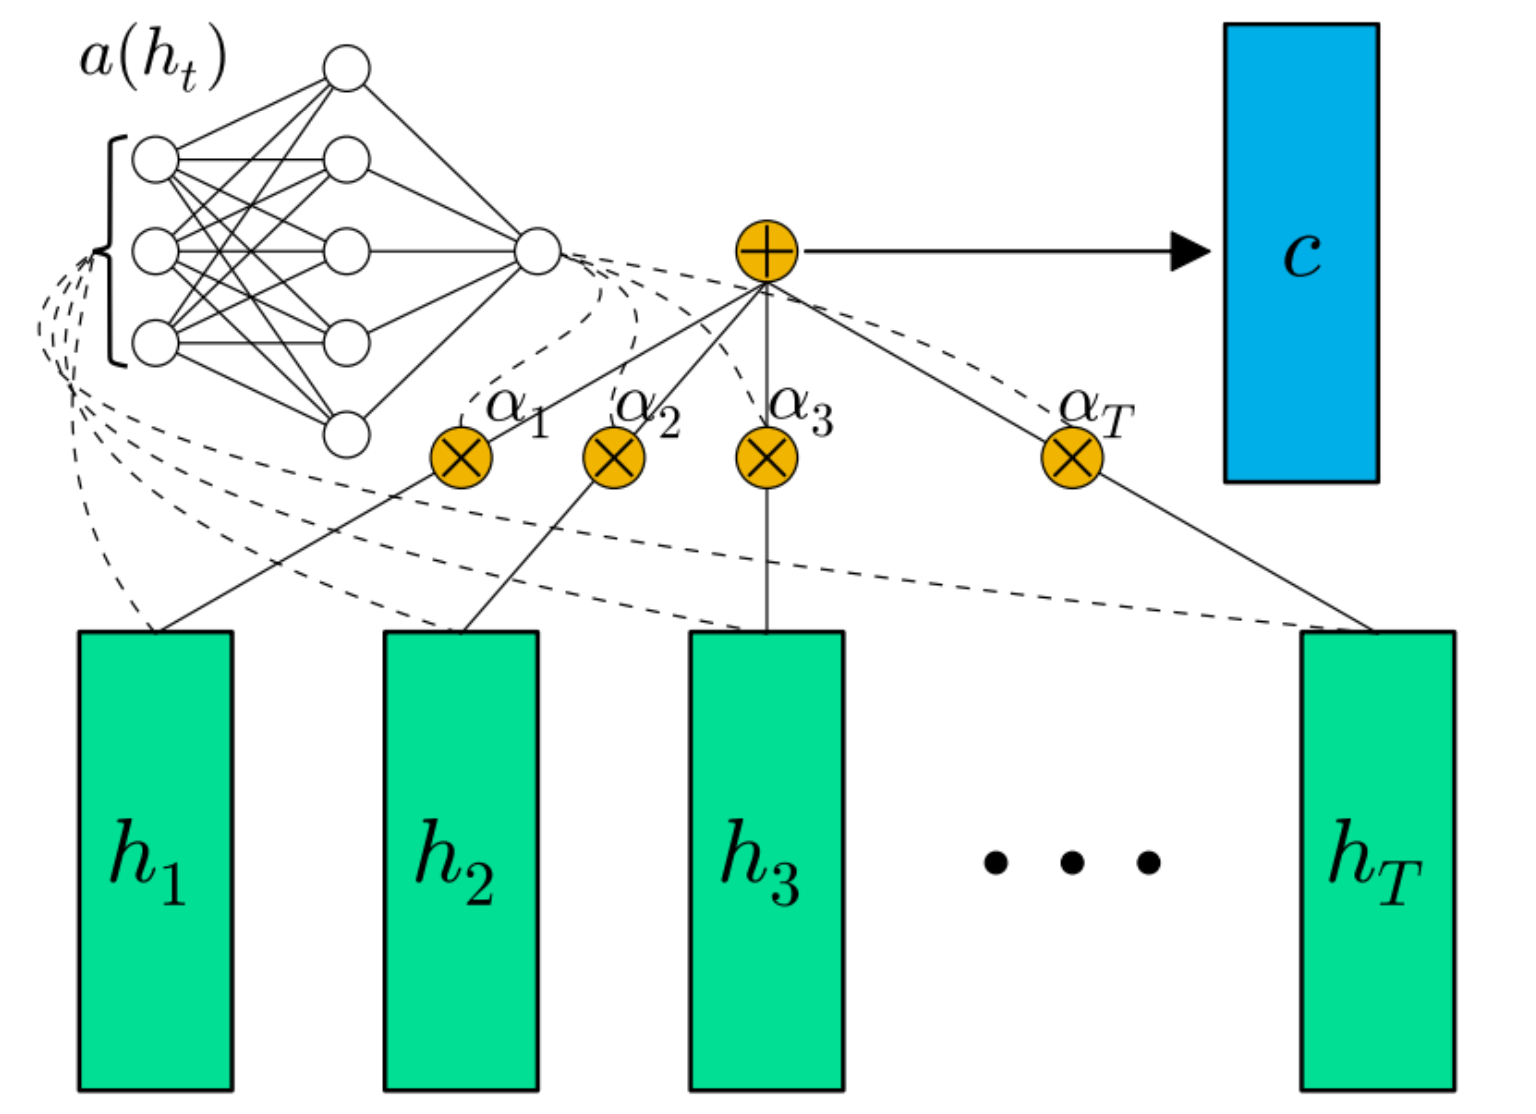
\includegraphics[width=0.5\linewidth]{img/attention_mechanism.png}
    
    
\end{figure}

\begin{figure}[H]
    \centering
    \includegraphics[width=0.75\linewidth]{img/attention_mechanism_example.png}
\end{figure}

The attention mechanism allows for inspecting and interpreting the model behaviour, as seen in the correlation matrix and the highlighted colour.

\section{Self-Attention Mechanisms in Transformers}
The Transformer model is a major improvement in neural network design for sequence-to-sequence tasks, using self-attention mechanisms for high parallelisation and efficiency.

\subsection{Transformer Model Overview}
\begin{itemize}
    \item The Transformer adopts an encoder-decoder structure shown in Figure \ref{fig:transformer_diagram} which processes tokenised input in the form of vector embeddings. 
    \item Positional encodings are added to the input embeddings to maintain the order of the words, as the self-attention mechanism does not inherently capture sequential information.
    \item It allows for parallel processing of words, which significantly improves efficiency and training speed compared to sequential models like RNNs and LSTMs.
\end{itemize}



\begin{figure}[H]
    \centering
    \begin{subfigure}[b]{0.4\textwidth}
        \includegraphics[width=\linewidth]{img/transformer.png}
        \caption{A transformer diagram. The left half is the encoder, and the right half is the decoder.}
        \label{fig:transformer_diagram}
    \end{subfigure}
        \begin{subfigure}[b]{0.5\textwidth}
        \includegraphics[width=\linewidth]{img/scaled_dot_prod_attn.png}
        \caption{Scaled dot-product attention}
        \label{fig:scaled_dot_prod}
    \end{subfigure}
\end{figure}

\subsection{Encoder Structure}
\begin{itemize}
    \item The Transformer model consists of \(N\) identical encoder layers.
    \item Each encoder layer has a multi-head self-attention mechanism with eight attention heads that allow the encoder to focus on different parts of the input sequence.
    \item Residual connections around each sub-layer, followed by layer normalisation, help in mitigating the vanishing gradient problem.
    \item A feed-forward neural network with ReLU activation functions connects the layers.
    \item The final output of the encoder becomes the input to the decoder.
\end{itemize}
\subsection{Decoder Structure}
\begin{itemize}
    \item The decoder also has \(N\) identical layers and receives the encoder outputs along with the outputs from the previous decoder layer, shifted right.
    \item Masked multi-head attention layers in the decoder prevent the model from attending to future tokens during training.
    \item Similar to the encoder, each decoder layer has multi-head attention, feed-forward networks, residual connections, and layer normalisation.
\end{itemize}

\subsection{Self-Attention Mechanism}
\begin{itemize}
    \item Self-attention, or intra-attention, enables each position in the encoder to attend to all positions in the previous layer of the encoder — allowing the model to dynamically focus on different parts of the input sequence.
    \item The mechanism computes a set of attention scores using queries (Q), keys (K), and values (V) which are derived from the input vector \(x\):
    \begin{align*}
        Q = M_q x, \quad K = M_k x, \quad V = M_v x, \\
        \text{Attention}(Q, K, V) = \text{softmax}\left(\frac{QK^T}{\sqrt{d_k}}\right)V
    \end{align*}
    \item The attention scores determine the weighting of the values, with \(d_k\) being the dimension of the key vectors used for scaling to normalise the variance, as shown in Figure \ref{fig:scaled_dot_prod} 
    \item The output is a weighted sum that promotes relevant words and diminishes less relevant ones.
\end{itemize}

\subsection{Multi-Head Attention}
\begin{itemize}
    \item Multi-head attention consists of several self-attention layers running in parallel, allowing the model to focus on different parts of the input sequence simultaneously.
    \item It combines insights from different representational spaces, capturing varied aspects of the information.
    \item Despite the split into multiple heads, each with reduced dimensionality, the total computational cost remains similar to single-head attention with full dimensionality due to parallel computation.
    \item Outputs from all heads are concatenated and passed through a final linear layer to produce the final values.
\end{itemize}

Transformers, through self-attention and multi-head attention, provide a powerful and flexible mechanism for modelling sequences, enabling advanced capabilities in natural language processing tasks without the sequential computation limitations of previous architectures.

\subsection{Reading Links}

\begin{itemize}
    \item \href{https://arxiv.org/abs/1706.03762}{Attention Is All You Need, Vaswani et al.,2017. }
    \item Transformers deal with long-term dependencies better thatn LSTMs
    \item Encoder-Decoder structure favours it for machine translation
    \item Reference: see illustrated \href{http://jalammar.github.io/ illustrated-transformer/}{blog}
\end{itemize}

\chapter{Representation Learning and Autoencoders}

\section{Three Types of Learning}
\begin{itemize}
    \item \textbf{Supervised Learning: } 
    \begin{itemize}
        \item Use labelled data
        \item Direct feedback
        \item Predict outcome or future
    \end{itemize}
    \item \textbf{Unsupervised Learning: } 
    \begin{itemize}
        \item No data labels
        \item No feedback
        \item Find a hidden structure or group (clustering)
    \end{itemize}
    \item \textbf{Reinforcement Learning: } 
    \begin{itemize}
        \item Decision Process
        \item Rewards System
        \item Learn a series of actions
    \end{itemize}
\end{itemize}

\subsection{Labelled or Unlabelled Data?}
\subsubsection{Supervised Learning Data Requirements}
The goal of supervised learning is to learn a relation between inputs and outputs $f:\mathcal{X}\to\mathcal{Y}$ for a given number of examples $(x_i,y_i)_{i=1}^n$, The more (usable) data, the better. But labelled data can be hard to come by.

\subsubsection{Unsupervised Learning to the Rescue?}
Unsupervised learning does not need labelled data – so it is usually inexpensive to collect large training sets.

Unsupervised data automatically finds relevant patterns in input data. It reduces the complexity of a supervised learning problem as it finds only useful features from the data and discarding what is unnecessary. 

\subsubsection{Semi-supervised Learning}
Semi-supervised learning is a branch of machine learning that combines supervised and unsupervised learning by using both labelled and unlabelled data to train models for classification and regression tasks.\\

It works based on the assumption that input data encodes useful properties about the input-output relation. It then can utilise both types of data to learn the shape of the larger data distribution.

\begin{figure}[H]
    \centering
    \includegraphics[width=0.5\linewidth]{img/image_face_dist.png}
    \caption{Pictures of human faces span a very low-dimensional subspace with respect to all possible images.}
\end{figure}

\subsection{Unsupervised Learning}
\begin{itemize}
    \item \textbf{Clustering: } Groups points according to common properties
    \item \textbf{Dimensionality Reduction: } Map points to a low dimensional space by keeping most of their relations unchanged
    \item \textbf{Density Estimation: } Approximate the distribution from the observed sample data, and try generate new examples of the data
    \item \textbf{Feature/Representation Learning: } Encode data within a concise but characteristic representation that can be used to solve other tasks e.g. classification, regression, etc
    \begin{figure}[H]
        \centering
        \includegraphics[width=0.5\linewidth]{img/cat_learning.png} 
    \end{figure}
\end{itemize}


\section{Sample Complexity}
The goal of supervised learning is to find the best function $f: \mathcal{X} \rightarrow \mathcal{Y}$ by minimising expected risk

\begin{equation}
    R(f)=\mathbb{E}\left.\ell(f(x),y)=\int_{X\times Y}\ell(f(x),y)\right.d\rho(x,y)
\end{equation}

Given an only finite number of training samples $S=\{(x_1,y_1)\ldots(x_n,y_n)\}$ sampled from $\rho.$
$\rho$ is the unknown data distribution and $\ell$ is the loss function (prediction error). Empirical risk minimisation helps find the best function given our data, by parametrising candidate solutions (for a feature space) as $f(x) = w^\top \phi (x)$, where $w \in \mathcal{H}_\phi$ is a vector of parameters (weights) in a feature space $\mathcal{H}_\phi$. Note that $\phi : \mathcal{X} \rightarrow \mathcal{H}_\phi$ is a feature representation.

\begin{equation}
    \hat{w}=\operatorname*{argmin}_{w\in\mathcal{H}_\phi}\frac1n\sum_{i=1}^n\ell(w^\top\phi(x_i),y_i)
\end{equation}

\begin{definitionbox}{Sample Complexity}
    One way to measure ERM with representation $\phi$ is the \textit{sample complexity}. \\

    It is defined by, for a given $\delta \in [0,1]$ and $\epsilon > 0$, the \textit{sample complexity} of an ERM with representation $\phi$ on a learning problem with data distribution $\rho$ is the minimum number $n_{\delta, \epsilon}(\rho, \phi)$ such that 
    \begin{equation}
        \mathbb{P}\left(R(\hat{w})-\inf_{f:\mathcal{X}\to\mathcal{Y}}R(f)<\varepsilon\right)\geqslant1-\delta 
    \end{equation}
    It is the minimum number of points needed to guarantee ERM performance to be as close as possible to the optimum one within bounds of $\epsilon$, with confidence $1-\delta$.

    The smaller the sample complexity, the better.
\end{definitionbox}

\begin{theorembox}{No Free Lunch Theorem}
\textbf{Basically: }there is no single best universal single feature representation. \\

For any feature representation \( \phi \), there is no guarantee that a small \( n(\rho, \phi) \) exists for all problems, i.e., there is no universal representation that works best for all possible distributions \( \rho \) that we might encounter.\\


The NFLT can be illustrated by considering two different problems, represented by two distributions \( \rho_1 \) and \( \rho_2 \), where the feature representation \( \phi \) leads to a small sample complexity \( n(\rho_1, \phi) \) but may not lead to a similarly small \( n(\rho_2, \phi) \). In essence, what works for one problem may not work for another if the underlying distributions of the data are significantly different.\\

In more formal terms, the NFLT states that the averaged performance of any two algorithms across all possible problems is identical. This implies that an algorithm that performs well on one class of problems must pay for it with degraded performance on the rest of the problems.\\

For any representation $\phi$, we have
\begin{equation}
    \text{sup}_\rho(\rho, \phi)= +\infty
\end{equation}


Overall, the No Free Lunch Theorem emphasises the importance of choosing the right model and representation for the specific problem at hand. It implies that while certain models may perform exceptionally well on certain tasks, their performance may degrade on others, and thus, no single model is superior in all contexts.\\

    \begin{figure}[H]
        \centering
        \includegraphics[width=0.65\linewidth]{img/no_free_lunch.png}
        \caption{Either one representation is good for discerning colours, or one representation is good for discerning shapes from others. But there is no universally best representation.}
    \end{figure}
\end{theorembox}

Since there is no best representation $\phi$ for any problem, it is better learn it for the unknown distribution at hand, $rho$ instead of assuming it \textit{a priori}. We can use unlabelled data points. This is the crux of Data Representation Learning, where for each $\phi$ we try to learn $\phi_\rho$.

\section{Representation Learning}
Goal: For feature representation $\phi$ and label predictor $g$, we want to learn $f(x) = g(\phi(x))$. $g$ requires output labels for learning, but $\phi$ does not. By utilising \textbf{reconstruction error}, it is a form of self-supervision.

Denote reconstruction error by 

\begin{equation}
\quad\|x-\psi(\phi(x))\|^2
\end{equation}

Where $\phi$ is now called feature encoding, and $\psi$ is feature decoding.

\begin{figure}[H]
    \centering
    \begin{subfigure}[b]{0.30\textwidth}
        \includegraphics[width=\linewidth]{img/supervised_comparison.png}
        \caption{Typical supervised learning with labelled data}
    \end{subfigure}
    \begin{subfigure}[b]{0.30\textwidth}
        \includegraphics[width=\linewidth]{img/representation_learning.png}
        \caption{Reconstruction of input given unlabelled data}
    \end{subfigure}
\end{figure}

$\phi$ captures more general properties of the data and can be used for other tasks. And learning it is inexpensive due to not requiring labelled data.

\subsection{Training Autoencoders}
Given dataset of $n$ points $(x_i)_{i=1}^n$, we want to solve
\begin{equation}
    \arg\min_{\phi,\psi}\frac1n\sum_{i=1}^n\|x_i-\psi(\phi(x_i))\|^2
\end{equation}

The issue is the trivial solution $\psi \circ \phi$, which is the identity function. For unconstrained $\phi$ and $\psi$ an autoencoder can `learn' all possible variability in training data, which is overfitting it in some sense. More formally, an autoencoder's latent representation captures all variability in the training data, which includes noise. Overfitting occurs when noise is learned instead of the optimum hypothesis that minimises loss.\\

This arises from the capacity of neural networks to approximate any function given enough parameters (as per the Universal Approximation Theorem). If the autoencoder simply learns the identity mapping, it will perfectly reconstruct the inputs without learning any useful or compressed representation of the data.\\

It is ideal to capture only key aspects in the data but ignore noise and nuances, in line with the Efficient Coding Hypothesis from the neuroscience of vision. 

\begin{definitionbox}{Efficient Coding Hypothesis}
    “...the Efficient Coding Hypothesis holds that the purpose of early visual processing is to produce an efficient representation of the incoming visual signal.”(Simoncelli ’03)
    \begin{figure}[H]
        \centering
        \includegraphics[width=0.5\linewidth]{img/ECH.png}
        
        
    \end{figure}
\end{definitionbox}

\section{Linear Autoencoders}
In general, this course considers Autoencoders wehre $\phi$ and $\psi$ are deep nets. However, the best way is to understand how shallow, linear autoencoders work. They have one hidden layer and no activation function.

Given a dataset of \( n \) points \( \{x_i\}_{i=1}^n \), the objective in training an autoencoder is to solve the following optimisation problem:

\begin{equation}
    \min_{\phi, \psi} \frac{1}{n} \sum_{i=1}^{n} \|x_i - \psi(\phi(x_i))\|^2
\end{equation}

where \( \phi : \mathbb{R}^d \to \mathbb{R}^r \) and \( \psi : \mathbb{R}^r \to \mathbb{R}^d \) correspond to matrices \( F, P \in \mathbb{R}^{r \times d} \), such that:

\begin{equation}
    \psi(\phi(x)) = P^TFx
\end{equation}



Note that the matrix \( P^TF \) is \( d \times d \) of rank at most \( r \leq d \). If \( r < d \), then \( P^TF \) cannot be the identity matrix.

The problem of training a linear Autoencoder becomes,

\begin{equation}
    \min_{P, F \in \mathbb{R}^{d \times r}} \frac{1}{n} \sum_{i=1}^{n} \|x_i - P^T Fx_i\|^2 = \min_{P, F \in \mathbb{R}^{d \times r}} \frac{1}{n} \|\mathbf{X} - P^T F\mathbf{X}\|_F^2
\end{equation}

Here, \( \mathbf{X} = [x_1, \ldots, x_n] \in \mathbb{R}^{d \times n} \) is the matrix concatenating the input data, and \( \|\mathbf{M}\|_F^2 = \text{Tr}(\mathbf{MM}^T) \) is the squared Frobenius norm of a matrix \( \mathbf{M} \) (sum of squared entries).


\begin{theorembox}{Principal Component Analysis}
    The solution $\hat{P} ^T \hat{F}$ encodes the first $r$ principal components of the data.\\

    $P ^\top F$ is learning an orthogonal projector onto a linear subspace of dimension $r$. 
    \begin{enumerate}
    \item Set the derivative of the objective function with respect to \( F \) to zero:
    \[ 0 = \nabla_F \|X - P^T FX\|_F^2 = 2P(X - P^T FX)X^T = 2(P - PP^T F)XX^T \]
    
    \item Solving \( P - PP^T F = 0 \) gives us \( F = (P^T P)^{+}P = (P^T)^+\), the psuedoinverse of $P^T$.
    
    \item Hence, we have \( P^T F = P^T (P^T )^{+} = \Pi \) which is an orthogonal projector onto the range of \( P \).
\end{enumerate}

Given that \( \Pi = P^T F \) is an orthogonal projector, we have \( \Pi^2 = \Pi \), and it can be associated with the first \( r \) principal components of \( X \).

\begin{enumerate}
    \item For a projector \( \Pi \), we have \( \Pi^2 = \Pi \). Hence, \( (I - \Pi)(I - \Pi) = I - \Pi \).
    
    \item Therefore, the reconstruction error simplifies to:
    \[ \|X - P^T FX\|_F^2 = \|(I - \Pi)X\|_F^2 = \text{Tr}(X^T (I - \Pi)X) \]
    
    \item Recall that an orthogonal projector of rank \( r \) can be written as \( \Pi = UU^T \), where \( U \) is a matrix with orthonormal columns.
    
    \item Hence, the trace simplifies further:
    \[ \text{Tr}(X^T (I - \Pi)X) = \text{Tr}(X^T X) - \text{Tr}(X^T UU^T X) \]
\end{enumerate}

The training of an autoencoder can be recast as a matrix factorisation problem:

\begin{equation}
\min_{F,P} \|X - P^T F\|_F^2 = \min_{U \in \mathbb{R}^{d \times r}, U^T U = I} \text{Tr}(X^T X) - \text{Tr}(U^T X^T X U) = \max_{U \in \mathbb{R}^{d \times r}, U^T U = I} \text{Tr}(U^T X^T X U)
\end{equation}

Here, the trace of \( U^T X^T X U \) is given by:

\begin{equation}
\text{Tr}(U^T X^T X U) = \sum_{j=1}^{r} u_j^T X^T X u_j,
\end{equation}


with \( u_j \) being the \( j \)-th column of \( U \).

Recall that \( \max_{||u||=1}u^T X^T X u \)  is attained by the first principal component of \( X \). Thus, the optimisation problem becomes:

\begin{equation}
\min_{F,P} \|X - P^T F\|_F^2 = \max_{U^T U = I} \sum_{j=1}^{r} u_j^T X^T X u_j,
\end{equation}

which is equivalent to finding the first \( r \) principal components of \( X \).


    
\end{theorembox}

\subsection{Nonlinear Features}
When working with linear encoders, we can consider a feature transformation $\phi$ to capture non-linear relations in the data, if we know such nonlinear relations beforehand. 

\begin{figure}[H]
    \centering
    \includegraphics[width=0.5\linewidth]{img/PCA_transform.png}
\end{figure}

If $\phi$ is not known, a deep, nonlinear autoencoder can be used to learn it.

\begin{figure}[H]
    \centering
    \includegraphics[width=0.5\linewidth]{img/d_nonlinear_autoencoder.png}
    
    
\end{figure}
\chapter{Generative Models}
\chapter{Reinforcement Learning}
\chapter{Interpretable and Trustworthy Models}



\end{document}

